\documentclass[a4paper]{scrartcl}
\usepackage[utf8]{inputenc}
\usepackage{ngerman}
\usepackage{mathtools}
\usepackage{amssymb}
\usepackage{pdfpages}
\usepackage{mathtools}
\usepackage{tikz}
\usepackage{ulem}
\usepackage{hyperref}

\title{Skriptum Mathematik 1}
\date{WS 2013/2014}
\author{Markus Klemm.net}

\begin{document}
\maketitle

\tableofcontents

\section{Elementare Grundlagen}
\subsection{Aussagen und Grundzüge der Logik}
\subsubsection{Aussagen, Wahrscheinlichkeitswert}
Aussagen sind zweitwertig. bool Aussage.

Bezeichnungen: p,q

Wahrheitswert $(p) =\left\{ \begin{array}{rcl}
         1
         & \mbox{falls}
         & \text{wahr} \\ 
         0  
         & \mbox{falls} 
         & \text{falsch} \\
                \end{array}\right.
                $

Beispiel: 
"`42 ist die Antwort auf alle Fragen"'
"`Diese Aussage ist falsch."' Nicht zweiwertig, ergo keine Aussage.

$p \underbrace{\equiv}_{\text{Identisch} \rightarrow \text{gleicher Wahrheitswert}} q$
\subsubsection{Aussagenlogik/-verbindungen}
\begin{enumerate}
\item Negation $\overline{p} \quad (p' , \neg p )$
\item Konjunktion $p \wedge q$ (Und)
\item Disjunktion $p \vee q$ (Oder)
\item Implikation $\underbrace{p}_{\text{Prämisse}} \rightarrow \underbrace{q}_{\text{Konklusion}} := (\overline{p} \vee q)$
\item Äquivalenz $p \leftrightarrow q := (p\rightarrow q) \wedge (q \rightarrow p)$
\end{enumerate}
\subsubsection{Logische Gesetze Tautologien}
Eine Tautologie $t$ ist eine Aussagenverbindung die unabhängig vom Wahrheitswert der einzelnen Aussagen stets wahr ist $t \equiv 1$

\subparagraph{Beispiele}
\begin{enumerate}
\item $p \leftrightarrow \overline{\overline{p}}$
\item $p\wedge \overline{p}$
\item
\begin{enumerate}

\item $\overline{p \wedge q} \leftrightarrow \overline{p}\vee \overline{q}$ (1. Regel von de Morgan)
\item $\overline{p\vee q} \leftrightarrow \overline{p} \wedge \overline{q}$ (2. Regel von de Morgan)
\end{enumerate}
\item $(p \rightarrow q) \leftrightarrow (\overline{q} \rightarrow \overline{p})$
\item $(p \wedge (p \rightarrow q)) \rightarrow q$ (direkter Beweis)
\item $(p \wedge (\overline{q} \rightarrow \overline{p}))\rightarrow q$ (indirekter Beweis)
\end{enumerate}

Bemerkung: Eine Äquivalenz ist genau dann eine Tautologie, wenn beide Seiten identisch sind, z.B. $p \equiv \overline{\overline{p}}$

\subparagraph{Beweistechniken} Zu beweisen: $q$
\begin{enumerate}
\item Direkter Beweis: Vorraussetzung $p, \quad p \rightarrow q$
\item Indirekter Beweis: Annahme $\overline{q}$ auf Widerspruch führen\\
\begin{equation*}
(\overline{q} \rightarrow q) \rightarrow q
\end{equation*}
\begin{equation*}
(\overline{q} \rightarrow 0 ) \rightarrow q
\end{equation*}
\end{enumerate}

\paragraph{Weitere Gesetze}
\begin{itemize}
\item $p \wedge q \equiv q \wedge p, \quad p \vee q \equiv q \vee p$ (Kommutativ)
\item $(p\wedge q) \wedge r \equiv p \wedge (q \wedge r ) \dots$ (Assoziativ)
\item $(p\wedge q)\vee r \equiv (p \vee r) \wedge (q \vee r) \dots$ (Distributiv)
\item $p \vee (p \wedge q) \equiv p$ (Absorptionsgesetz)
\end{itemize}
\subsubsection{Aussagenfunktionen, Quantoren, Prädikatenlogik} %1.1.4

$\chi$ sei eine Menge (Gesamtheit von Objekten x mit einem gemeinsamen Merkmal, vgl. Abschnitt 1.2.)

$x \in \chi$ \dots x ist Element von $\chi$.
Die Objekte haben Eigenschaften (Prädikate).
Aussagenfunktion (auch Aussagenform) $p(x)$:
Jedem $x \in \chi$ ist eine Aussage $p(x)$ zugeordnet.
Dabei steht x für ein Element, p für ein Prädikat.

Beispiel 5:
$\chi$ \dots Menge der positiven natürlichen Zahlen; 1,2,3, \dots
$p(x) :=$ "`x ist eine Primzahl"'
z.B. p(5) wahr, p(10) falsch

\paragraph{Quantoren}
Betrachtet werden folgende Aussagen
\begin{enumerate}
\item Für alle x (aus $\chi$) gilt p(x):
Bezeichung $\forall_x p(x)$ (universeller Quantor, Allquantor)
\item Es existiert (mindestens) ein x, für welches p(x) gilt:
Bezeichnung $\exists_x p(x)$ (existenzieller Quantor)
\end{enumerate}
\paragraph{Zur Schreibweise}
Bei Anwendungen (außerhalb der reinen Logik) wird oft die Grundmenge $\chi$ mit angegeben:
$\forall_{x \in \chi} p(x)$ usw.
Falls sich Quantoren auf eine Teilmenge M von $\chi$ bezeichnen sollen, können dann folgende Schreibweisen verwendet werden:
$a= \forall_{x\in M} \quad p(x), b=\exists_{e\in M} \quad p(x)$
Die Schreibweisen in der folgenden Logik sind dann:
$a=\forall_x (x \in M \Rightarrow p(x)), b = \exists_x (x\in M \wedge p(x))$
\paragraph{Rechenregeln}
\[\overline{\forall_x p(x)} \equiv \exists_x \overline{p(x)}\]
\[\overline{\exists_x p(x)} \equiv \forall_x \overline{p(x)}\]
\paragraph{Mehrstellige Aussagenfunktionen}
\begin{itemize}
\item $p (x1,x2,...,x_n), x_1 \in \chi_1,...,x_n\in \chi_n$
(Grundmengen $\chi_i$ können gleich sein, müssen es aber nicht)
\item Wird ein Quantor auf eine n-stellige Aussagenfunktion angewandt, so entsteht eine (n-1)-stelle Aussagenfunktion. (Dabei 0-stellige Aussagenfunktion $\rightarrow$ Aussage)
z.B: $\exists_y p(x,y,z)$ , die Varaiable y wird durch den Quantor $\exists$ gebunden $\rightarrow$ gebundene Variable, x und z sind freie Variablen $\exists_y p(x,y,z) = q(x,z)$
Beispiel 6: Ein Dorf bestehe aus 2 Teilen (Ober- und Unterdorf). Es sei M die Menge aller Bewohner des Dorfes. $M_1$ bzw. $M_2$ sei die Teilmengenv von $M$, die dem Oberdorf bzw. Unterdorf entsprechen. Wir betrachten folgende zweistellige Aussagenfunktion
$k(x,y)$ \dots Person $x$ (aus $M$) kennt Person $y$ (aus $M$)
\end{itemize}
\subsection{Mengen}%1.2.
\subsubsection{Begriffe}%1.2.1
\paragraph{Menge} Zusammenfassung gewisse Objekte (Elemente) mit einem gemeinsamen Mermal zu einem Ganzen
\paragraph{Diskusion} Naiver Mengenbegriff, führt zu Widersprüchen. Diese können umgangen werden, wenn nur Teilmengen einer sogenannten Grundmenge betrachtet werden.

Bezeichnung meist mit großen Buchstaben A,B,...,M
$x \in M$ \dots $x$ ist Element von $M$
$x \notin M$ \dots $x$ ist kein Element von $M$

Schreibweise $M=\{ \dots\}$ oder $M=\{ x \vert  p(x)\}$

Wichtige Grundmengen:

$\mathbb{N}$ \dots Menge der natürlichen Zahlen \{0,1,2,3,...\} \\
$\mathbb{N}^* = \{1,2,3,...\} = \mathbb{N} \backslash \{0\}$

Beispiel 1: 
\begin{enumerate}
\item $M_1$ \dots Menge der Primzahlen kleiner als 10, \\
$M_1 = \{ 2,3,5,7\}$
\item $M_2 = \{ x \in \mathbb{R} \vert 0 < x < 1\} =: (0;1)$ \dots Intervallschreibweise
\end{enumerate}
\paragraph{Definition 1}
Es seien a und b reelle Zahlen mit $a < b$. \\
$[a;b] :=\{ x \in \mathbb{R} \vert a \leq x \leq b\}$ \dots abgeschlossenes Intervall\\
$(a;b) :=\{ x \in \mathbb{R} \vert a < x < b\}$ \dots offenes Intervall\\
$[a;b) :=\{ x \in \mathbb{R} \vert a \leq x < b\}$\\
$(-\infty ; a] := \{ x \in \mathbb{R} \vert -\infty < x \leq a \} = \{ x \in \mathbb{R} \vert x \leq a \}$ usw.

\subparagraph{Leere Menge}
z.B. $ \{ x \in \mathbb{R} \vert x=x+1\}$ enthält kein Element, Bezeichnung $\varnothing $ (oder \{ \} )



\subsubsection{Mengenverknüpfungen}
\paragraph{Definition 2}
$M_1 = M_2 \quad := \forall X (x \in M_1 \leftrightarrow x \in M_2)$ (Gleichheit)
\paragraph{Definition 3}
$M_1 \subseteq M_2 \quad := \forall X ( x\in M_1 \rightarrow x \in M_2)$ (Inklusion)\\*
"`$M_1$ ist Teilmenge von $M_2$"'
\paragraph{Diskussion}
Ist $M_1 \subseteq M_2$, aber $M_1 \neq M_2$ So kann man schreiben $M_1 \subset M_2$ (Echte Teilmenge)
\paragraph{Definition 4}
\begin{enumerate}
\item $A \cap B :=\{x \vert x \in A \wedge x \in B\}$\\*
Durchschnitt von A und B
\item $A \cup B :=\{ x \vert x \in A \vee x \in B\}$\\*
Vereinigung von A und B
\item $A \backslash B := \{x \vert x \in A \wedge x \notin B\}$\\*
Differenz "`A minus B"'
\item Beim Vorliegen einer Grundmenge E: \\*
$\overline{A} := E \backslash A$\\*
Komplementärmenge von A
\end{enumerate}
\paragraph{Diskussion}
\begin{enumerate}
\item $\cup$ und $\cap$ sind kommutativ und assoziativ, z.B. gilt $A\cup B = B \cup A, (A\cap B)\cap C = A\cap (B\cap C)=: A \cap B \cap C$
\item Allg. I \dots Indexmenge, z.B. $\{1,2,...,n\}, \mathbb{N},\mathbb{Z}, \\*
$ dann $\bigcap\limits_{i \in I} A_i := \{ x \vert \exists_{i\in I} X \in A_i\} $\\*
$\bigcup\limits_{i \in I} A_i := \{ x \vert \forall_{i \in I} x \in A_i\}$
\end{enumerate}


\subsubsection{Relationen}
\paragraph{Grundbegriffe}
\subparagraph{Definition 5}
Die Menge $M_1 \times M_2 :=\{(x_1,x_2)\vert x_1 \in M_1 \wedge x_2 \in M_2\}$\\*
heißt kartesisches Produkt der Mengen $M_1$ und $M_2$. (= Menge ungeordneter Paare)
\subparagraph{Beispiel 2}
$\mathbb{R}$ \dots Menge der reellen Zahlen veranschaulicht durch die Zahlengerade\\*
$\mathbb{R}^2 := \mathbb{R} \times \mathbb{R} = \{ (x,y) \vert x \in \mathbb{R} \wedge y \in \mathbb{R}$ \dots x-y-Ebene
\subparagraph{Definition 6}
Eine Teilmenge $T\subseteq M_1 \times M_2$ heißt binäre Relation.
\subparagraph{Diskussion}
\begin{enumerate}
\item Verallgemeinerung\\*
$M_1 \times M_2 \times ... \times M_n = \{(x_1,x_2,...,x_n) \vert x_1 \in M_1, x_2 \in M_2, ..., x_n\in M_n\}$\\
=Menge der geordneter n-Tupel), eine Teilmenge $T\subseteq M_1 \times M_2 \times ... \times M_n$ heißt n-stellige Relation
\item Jede Teilmenge von $M_1 \times M_2$ ist eine Relation, also auch die beiden Grenzfälle $\varnothing$ und $M_1 \times M_2$. Wichtig sind aber im Allgemeinem die echten Teilmengen, die die verschiedensten Beziehungen zwischen den Elementen von $M_1$ und $M_2$ ausdrücken.
\end{enumerate}
\subparagraph{Definition 7}
Eigenschaften binärer Relationen in $M_1 \times M_2$\\
Eine Relation $T \subseteq M_1 \times M_2$ heißt:
\begin{enumerate}
\item linksvollständig (linkstotal), wenn für jedes $x_1 \in M_1$ wenigstens ein $x_2 \in M_2$ existiert mit $(x_1,x_2)\in T$\label{def7a}
\item rechtsvollständig (rechtstotal), wenn für jedes $x_2 \in M_2$ wenigstens ein $x_1 \in M_1$ existiert mit $(x_1,x_2) \in T$
\item rechtseindeutig, wenn für jedes $x_1 \in M_1$ höchstens ein $x_2 \in M_2$ existiert mit $(x_1,x_2) \in T$\label{def7c}
\item linkseindeutig, wenn für jedes $x_2 \in M_2$, höchstens ein $x_1 \in M_1$ existiert mit $(x_1,x_2) \in T$
\end{enumerate}
\subparagraph{Definition 8} Eigenschaften binärer Relationen in $M \times M$\\
Eine Relation $T\subseteq M\times M$ (Sprechweise auch Relation auf M) heißt
\begin{enumerate}
\item reflexsiv, wenn $(x,x) \in T$
\item symetrisch, wenn $(x,y) \in T \rightarrow (y,x) \in T$
\item antisymetrisch, wenn $((x,y)\in T \wedge (y,x) \in T) \rightarrow x=y$
\item asymetrisch, wenn $(x,y) \in T \rightarrow  (y,x) \notin T$
\item transitiv, wenn $((x,y) \in T \wedge (y,z) \in T) \rightarrow (x,z) \in T$
\end{enumerate}
jeweils $\forall x,y,z \in M$ gilt.

Zwei Personen $x \in P$ und $y \in P$ heißen gleichaltrig, wenn x und y das gleiche Geburtsjahr besitzen.
Relation $G \subseteq P \times P$ mit $ G =\{ (x,y) \vert$ x und y sind gleichaltrig\}\\
G ist offensichtlich reflexiv, symmetrisch und transitiv.
Derartige Relationen nennt man Äquivalenzrelationen. (vlg. 1.2.3.3). Sie teilen P in disjunkte sog. Äquivalenzklassen auf. (x äquivalent y, heißt x und y besitzen gleiches Geburtsjahr).

\paragraph{Grafische Darstellung von Relationen $T$ in $M \times M$ (auf $M$)}

\paragraph{1.Möglichkeit:} Elemente von M nur einmal darstellen, Pfeildarstellung wie bisher, bei $(x,x)\in T$ eine Schlinge zuordnen.
$x_\circlearrowleft \rightarrow y \rightleftarrows z$
\subparagraph{Reflexivität}Bei jedem Element eine Schlinge ( $\circlearrowleft$ )
\subparagraph{Symmetrie}Jeder Pfeil $x \rightleftarrows y (x \neq y)$
besitzt Umkehrpfeil (Antisymmetrie: Schlingen sind möglich, aber keine Umkehrpfeile, Asymmetrie: Weder Schlingen noch Umkehrpfeile)
\subparagraph{Transitivität} Falls Pfeil $x \rightarrow y$ eine Fortsetzung $y \rightarrow z$ besitzt, dann verläuft auch ein Pfeil von x nach z.

\paragraph{2.Möglichkeit:} Mit Koordinatensystem

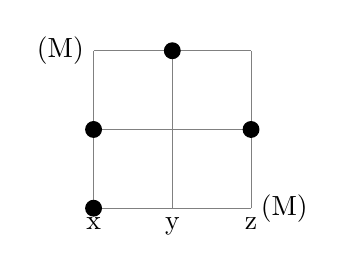
\begin{tikzpicture}
\draw[help lines] (0,0) grid (2,2);
\node [below] at (0,0) {x}; \node [below] at (1,0) {y}; \node [below] at (2,0) {z};
\node [left] at (0,2) {(M)};\node [right] at (2,0) {(M)};
\draw[fill] (0,0) circle [radius=0.1];
\draw[fill] (0,1) circle [radius=0.1];
\draw[fill] (1,2) circle [radius=0.1];
\draw[fill] (2,1) circle [radius=0.1];

\end{tikzpicture}
\subparagraph{Reflexivität} Die Diagonale $I_M = \{(x,x) \vert x\in M\}$ gehört zu $T$ ($I_M$ heißt auch Identitätsrelation, diese Relation ist eine spezielle Funktion)
\subparagraph{Symmetrie}T ist spiegelsymmetrisch zu $I_M$

\paragraph{Alternative Schreibweisen}
Es sei $T \subseteq M_1 \times M_2$ eine binäre Relation. An Stelle $(x,y) \in T$ kann man auch schreiben:
\begin{enumerate}
\item $x \; T \; y$
(x steht in Relation T zu y), für viele Relationen gibt es spezielle Zeichen z.B. $x < y$, $g || h$.
\item Aussagenfunktion (vlg. Prädikatenlogik) $T(x,y)$ (auch mehrstellig möglich) 
\end{enumerate}

\paragraph{Operationen auf Relationen}

Da Relationen spezielle Mengen sind, gibt es die Operation $\cap \cup$ usw. auch hier. Weitere für Relationen typische Operationen vgl. Definition 9-11.

\subparagraph{Definition 9} Es sei $T$ eine Relation in $U\times V$\\
Die Menge
\[proj_1 (T) = \{ x \in U | \exists y\in V \quad (x,y) \in T\}\]
heißt Projektion von T auf U. (1. Faktor des Produkts)\\
Analog ist
\[ proj_2 (T) = \{ y \in V | \exists x \in U \quad (x,y) \in T\}\]
die Projektion von $T$ auf den 2. Faktor ($V$) des Produkts $U\times V$.

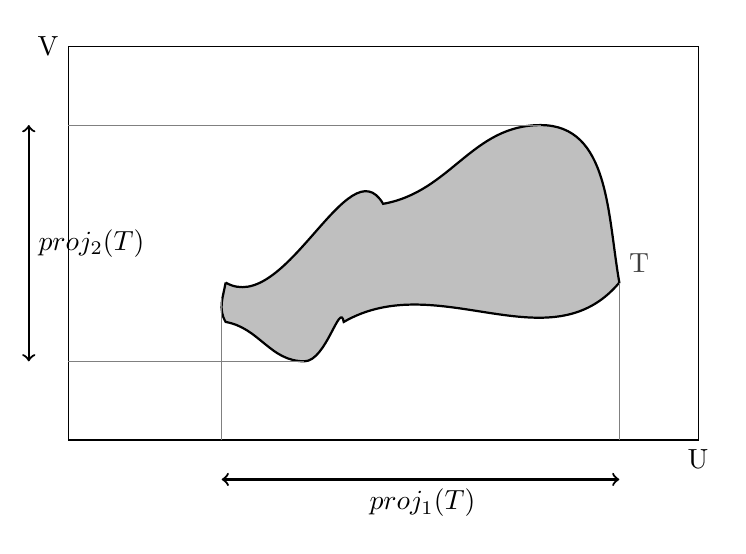
\begin{tikzpicture}


\draw [fill=lightgray,thick](2,2) to [out=-30,in=120] (4,3) to [out=10,in=180] (6,4) to [out=0,in=100] (7,2) to [out=230,in=30] (3.5,1.5) to [out=100,in=0] (3,1) to [out=180,in=-10] (2,1.5) to [out=120,in=260] (2,2);

\draw (0,0) rectangle (8,5);

\node [left] at (0,5) {V}; \node [above right,darkgray] at (7,2) {T}; \node [below] at (8,0) {U};

\draw [help lines] (0,1) -- (3,1); 
\draw [<->,thick] (-0.5,1) -- (-0.5,4); \node [right] at (-0.5,2.5) {$proj_2(T)$};
\draw [help lines] (0,4) -- (6,4);

\draw [help lines] (1.95,0) -- (1.95,1.8);
\draw [<->,thick] (1.95,-0.5) -- (7,-0.5); \node [below] at (4.5,-0.5) {$proj_1(T)$};
\draw [help lines] (7,0) -- (7,2);


\end{tikzpicture}

\subparagraph{Definition 10} Es sei $T \subseteq M_1 \times M_2$ eine binäre Relation\\
Die Relation
\[ T^{-1} := \{ (y,x) | (x,y) \in T\} \subseteq M_2\times M_1\]
heißt inverse Relation zu $T$ (kurz Inverse).

\paragraph{Definition 11} Es seien $T_1 \subseteq M_1 \times M_2$ und $T_2 \subseteq M_2 \times M_3$ binäre Relationen. Als Komposition (oder Verkettung) $T_1 \circ T_2$ wird folgende Relation
\[T_1 \circ T_2 :=\{(x,z)\in M_1 \times M_3 | \exists y \in M_2 \quad ((x,y) \in T_1 \wedge (y,z) \in T_2 )\}\]
in $M_1 \times M_3$ bezeichnet.

\subparagraph{Diskussion}
Wichtige Eigenschaft der Komposition $\circ$:
Die Operation $\circ$ ist assoziativ, d.h.  sei $T_1 \subseteq A \times B, T_2 \subseteq B \times C$ und $T_3 \subseteq C \times D$, dann gilt $(T_1 \circ T_2)\circ T_3 = T_1 \circ (T_2 \circ T_3) =:  T_1 \circ T_2 \circ T_3 \subseteq A \times D$


\subparagraph{Definition 12}
Es sei $T$ eine Relation in $M \times M$ (auf M). Als transitive Hülle $T^+$ von $T$ bezeichnet man die kleinste Relation die $T$ enthält und transitiv ist.

Satz 1
Es gilt 
\[T^+ = T \cup (T \circ T) \cup (T \circ T \circ T) \cup ...\]

\subparagraph{Bemerkung}
Bezeichnung für $\underbrace{T \circ T \circ ... \circ T}_{n-mal}$ auch $T^n$.

Achtung nicht zu verwechseln mit dem Mengenprodukt $T \times T\times ...\times T$ bzw. bei Funktion mit der n-ten Potenz $f^n$ Damit ist
\begin{equation*}
T^+ = \bigcup\limits_{g=1}^\infty T^j
\end{equation*}

Beweis:
\begin{enumerate}
\item $T^+$ ist transitiv, dann sei $(x,y) \in T^+ \wedge (y,z) \in T^+$, dann existiert natürliche Zahlen $j_1,j_2 \geq 1$ mit $(x,y) \in T^{j_1}$ und $(y,z) \in T^{j_2}$, d.h. y wird in $j_1$ Schritten von $x$ aus erreicht und $z$ in $j_2$ Schritten von $y$ aus.
Also wird $z$ in $j_1 + j_2$ Schritten von $x$ aus erreicht, d.h.:
$(x,z) \in T_{j_1 + j_2} \Rightarrow (x,z) \in T^+$.
\item Es sei $T \subseteq S$ für eine transitive Relation $S \Rightarrow T\circ T \subseteq S \circ S \subseteq S$ und für beliebiges $j \geq z$ \quad 
$ T^j \subseteq S^j \subseteq S$ und damit $T^+ = \bigcup\limits_{g=1}^{\infty} T^j \subseteq S$, d.h. $T^+$ ist tatsächlich die kleinste transitive Relation, die $T$ enthält.
\end{enumerate}
\subparagraph{Diskussion}
\begin{enumerate}
\item Analog zur transitiven Hülle einer RElation $T$ in $M \times M$ (auf M) werden die reflexive bzw. die symmetrische Hülle als die jeweils kleinsten Relationen, die T enthalten und die entsprechende Eigenschaft besitzen, erklärt. Die Ermittlung gestattet sich etwas einfacher als bei der transitiven Hülle.

Reflexive Hülle von $T$:
\[T\cup I_M\]
dabei $I_M =\{ (x,x) | x \in M\}$ \dots Identitätsrelation.

Symmetrische Hülle von $T$:
$T \cup T^{-1}$
\item Von Bedeutung ist auch die reflexiv-transitive Hülle von $T: \quad T^* := T^+ \cup I_M$
(dabei $T^*$ transitive Hülle)
\end{enumerate}

\subparagraph{Beispiel 8} Gegeben sei die Menge $M =\{ a,b,c,d,e,f\}$ sowie die Relation\\* $T=\{(a,b,),(b,c),(c,e),(b,d),(d,e),(e,f)\}$
\begin{enumerate}
\item Transitive Hülle

Zur Ermittlung der Elemente eines Komposition $S \circ T$: Für jedes Element $(x,y)\in S$ alle Fortsetzungen $(y,z_i)\in T$ suchen $\curvearrowright (x,z_i)$ als Element von $S \circ T$ notieren, falls noch nicht vorhanden.

Also $T\circ T: (a,b)$ Fortsetzung $(b,c),(b,d) \curvearrowright (a,c),(a,d)$ \\* $(b,c)$ Fortsetzung $(c,e) \curvearrowright (b,c)$\\
$\curvearrowright T \circ T = T^2 = \{(b,c,),(b,d),(c,e),(c,f)$
$\curvearrowright T^3 = T\circ T^2=\{(a,e),(b,f)\}$
$\curvearrowright T^4 = T\circ T^3 =\{ (a,f)\}$
$\curvearrowright T^5 = T\circ T^4 = \varnothing \curvearrowright T^+ = T\cup T^2 \cup T^3 \cup T^4$

\item Reflexive Hülle: $T\cup \{(a,a),(b,b),(c,c),(d,d),(e,e),(f,f)\}$
\item Symmetrische Hülle: $T\cup T^{-1} = T \cup \{(b,a),(c,b),...\}$
\end{enumerate}

Zur Überprüfung der Eigenschaften aus Definition 8 ist folgender Satz nützlich:
\subparagraph{Satz 2} Es sei $T \subseteq M \times M$ eine binäre Relation. Dann gilt:
\begin{enumerate}
\item $T$ ist reflexiv $\Leftrightarrow I_M \subseteq T$ ($I_M$ \dots Identitätsrelation)
\item $T$ ist symmetrisch $\Leftrightarrow T^{-1} \subseteq T ( \Leftrightarrow T^{-1} = T)$
\item $T$ ist antisymmetrisch $\Leftrightarrow T \cap T^{-1} \subseteq I_M$ \label{c)}
\item $T$ ist asymmetrisch $\Leftrightarrow T \cap T^{-1} = \varnothing$
\item $T$ ist transitiv $\Leftrightarrow T\circ T \subseteq T$
\end{enumerate}

\subparagraph{Diskussion} Aus c) und d) ergibt sich
\begin{quote}
T asymmetrisch $\Rightarrow$ T antisymmetrisch
\end{quote}
(da $\varnothing$ Teilmenge jeder Menge ist, auch von $I_M$)

\paragraph{Äquivalenzrelationen}
\subparagraph{Definition 13}
Eine Relation $T \subseteq M \times M$ heißt Äquivalenzrelation, wenn sie reflexiv, symmetrisch und transitiv ist:

Diskussion:
\begin{enumerate}
\item Durch eine Äquivalenzrelation wird $M$ vollständig in paarweise elementfremde (disjunkte) Äquivalenzklassen zerlegt. Die Menge aller Äquivalenzklassen von $M$ bezüglich $T$ heißt Quotientenmenge $M/T$.

Aufgrund der 3 Eigenschaften aus Definition 13 enthält eine Äquivalenzklasse alle Elemente die untereinander erreichbar sind und nur diese.

\item Äquivalenzklassen enthalten alle Elemente die bezüglich einer bestimmten Eigenschaft nicht unterscheidbar sind (= äquivalent), z.B. Beispiel 4b mit $M=P$ (Menge von Personen), Äquivalent $G \subseteq P \times P$ mit $\{ (x,y) |$ x u. haben gleiches Geburtsjahr\}, Äquivalenzklassen sind die Jahrgänge.

\item Anstelle der Schreibweisen $(x,y,)\in T, \quad \times T y$ oder $T(x,y)$ verwendet man bei beliebigen Äquivalenzklassen auch $x \sim y$. Bei vielen speziellen Äquivalenzrelationen spezielle Symbole, vlg. Beispiel 9.

\subparagraph{Beispiel 9}\label{Bsp9}
\begin{enumerate}
\item $M$ sei eine beliebige Menge $T_1 = I_M = \{ (x,y) \in M \times M | x=y\}$ (Identitätsrelation) ist eine Äquivalenzrelation. Äquivalenz heißt hier gleich!
Äquivalenzklassen sind sämtliche einelementige Teilmengen $\{x\} , x \in M$. $T_1$ liefert die feinste Zerlegung von M, die möglich ist. Die gröbste "`Zerlegung"' liefert die Relation $T_2 = M \times M$, die trivialerweise eine Äquivalenzrelation ist (mit nur einer Äquivalenzklasse M). Für die Anwendungen wichtig: Relationen, die eine echte Zerlegung liefern.

\item $M= \mathbb{Z}$ (ganze Zahlen), $m \in \mathbb{N}^*, T \subseteq \mathbb{Z} \times \mathbb{Z}$ mit
\begin {enumerate}
\item $(x,y) \in T :=$ "`x und y lassen bei Division den gleichen Rest"'
\item Bezeichnung $x \equiv y (\mod{m})$ x kongruent y (modulo m)
z.B. $29 \equiv 8 (\mod{7})$
\item $T$ ist eine Äquivlenzrelation auf $\mathbb{Z}$, Äquivalenzklassen: Restklassen (modulo M).
\end{enumerate}

\item $M$\dots Menge aller Geraden einer Ebene, $T\subseteq M \times M$ mit
$(x,y) \in T :=$ "`x ist parallel zu y"'.
Bezeichnung $x\parallel y$, T ist Äquivalenzrelation auf $M$.

\end{enumerate}
\end{enumerate}

\paragraph{Ordnungsrelation}%1.2.3.4.
\subparagraph{Definition 14}
\begin{enumerate}
\item Eine Relation $T \subseteq M \times M$ heißt Ordnungsrelation auf $M$, wenn sie reflexiv, antisymmetrisch und transitiv ist.
\item Eine Ordnungsrelation heißt vollständig (oder linear), wenn für alle $x,y \in M$ gilt $(x,y) \in T \vee (y,x) \in T$

\end{enumerate}

\subparagraph{Definition 15} Eine Relation $T \subseteq M \times M$ heißt strikte Ordnungsrelation, wenn sie asymmetrisch und transitiv ist. Eine strikte Ordnung heißt vollständig (linear), wenn für alle $x,y \in M$ mit $x\neq y$ gilt: $(x,y) \in T \wedge (y,x) \in T$

\subparagraph{Beispiel 10}
\begin{enumerate}
\item $M = \mathbb{R}, T \subseteq \mathbb{R} \times \mathbb{R}$ mit $(x,y)\in T := x \leq y$ ist eine vollständige Ordnungsrelation auf $\mathbb{R}$
\item Die Relation "`$<$"' ist eine vollständige, strikte Ordnung auf $\mathbb{R}$.
\item $E$ sei die Menge, $M$ sei die Menge aller Teilmengen von $E$, die sogenannte Potenzmenge $M = \mathcal P(E) \quad T \subseteq M \times M$ mit $(A,B) \in T := A\subseteq B$ ist eine Ordnungsrelation $\mathcal P(E)$ (Inklusion)

\end{enumerate}

Diskussion:
\begin{enumerate}
\item In der Literatur wird manchmal eine Relation im Sinne der Definition 14 als Halbordnung und nur eine vollständige Ordnung als Ordnungsrelation bezeichnet.
\item Zu jeder Ordnung $T_1$ (auf $M$) gehört eine strikte Ordnung $T_2$ und umgekehrt.
\[ T_2 = T_1 \backslash I_M \quad \text{bzw.} \quad T_1 = T_2 \cup I_M\]
($T_1$ ist die reflexive Hülle von $T_2$), z.B. $(\leq ,<)$ oder $(\subseteq , \subset )$
\item Die Symbole $\leq$ bzw. $<$ können anstelle der Paarschreibweise auch bei beliebigen Ordnungen verwendet werden, falls keine anderen Symbole vorhanden.

\end{enumerate}

\subparagraph{Definition 16} T sei eine Ordnungsrelation auf einer Menge $M$. Weiter sei $A$ eine Teilmenge von $M$.
\begin{enumerate}
\item Ein Element $a \in M$ heißt obere Schranken von $A$, wenn $\forall x \in A \quad x \leq a$, d.h. $(x,a) \in T$ vgl. Diskussion 3.
\item Es sei $B$ die Menge aller oberen Schranken von $A$ ($B\neq \varnothing$). Falls es eine kleinste obere Schranke $s$ von A gibt, d.h.
$\exists s \in B \forall b \in B \quad s\leq b$, so heißt $s$ das Supremum von $A$, $s = \sup{A}$
\item Gilt $s\in A$, so heißt $s$ das Maximum von $A$, $s=\max{A} = \sup{A}$
\item Ein Element $M \in A$ heißt maximal, wenn es kein größeres Element in $A$ gibt, d.h. $\forall x\in A \quad ( m \leq x \Rightarrow m=x)$

\end{enumerate}

Diskussion:
\begin{enumerate}
\item Die Begriffe aus Definition 16, lassen sich auf strikte Ordnungen $S$ übertragen, indem anstelle von $S$ die reflexive Hülle $S \cup I_M$ verwendet wird.
\item Bei Ordnugnsrelationen $T$ (auch strikten) auf endlichen Mengen $M$, kann ein vereinfachter Graph, das sogenannte \textsc{Hasse} -Diagramm betrachtet werden:
$a \rightarrow b (a\neq b)$ bedeutet $(a,b) \in T$ und es gibt kein Zwischenglied $c \neq a$ und $c \neq b$ mit $(a,c) \in T \wedge (c,b) \in T$, ($b$ ist unmittelbar Nachfolger von $a$ bzw. $a$ ist unmittelbar Vorgänger von $b$)

Diesem Diagramm entspricht eine Teilrelation $U \subseteq T$, deren transitiv-reflexive Hülle (bzw. transitive Hülle bei strikten Ordnungen) die Relation $T$ ist.
\item Veranschaulichung von Definition 16 mit einem \textsc{Hasse} Diagramm einer nicht-vollständigen Ordnung (nicht linear)

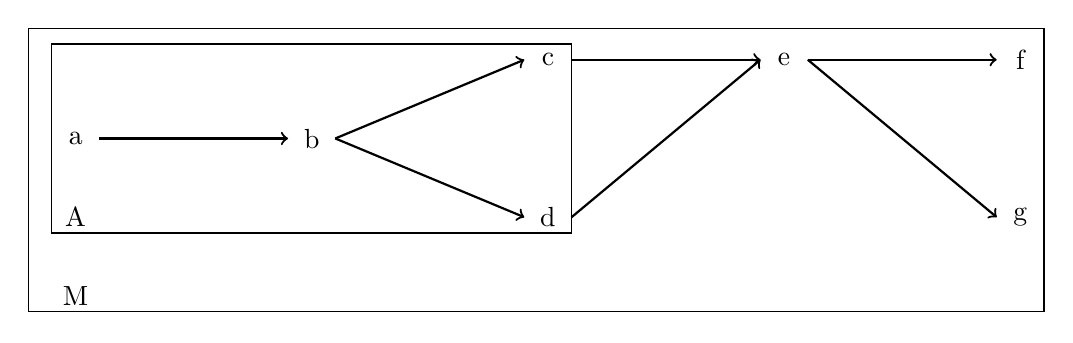
\begin{tikzpicture}[xscale=3]
%\draw [help lines] (0,0) grid (4,3);
\node at (2,3) {c}; \draw [->,thick] (2.1,3) -- (2.9,3); \node at (3,3) {e}; \draw [->,thick] (3.1,3) -- (3.9,3); \draw [->,thick] (3.1,3) -- (3.9,1); \node at (4,3) {f};
\node at (0,2) {a}; \draw [->,thick] (0.1,2) -- (0.9,2); \node at (1,2) {b}; \draw [->,thick] (1.1,2) -- (1.9,3); \draw [->,thick] (1.1,2) -- (1.9,1);
\draw (-0.1,0.8) rectangle (2.1,3.2);  \node at (0,1) {A}; \node at (2,1) {d}; \draw [->,thick] (2.1,1) -- (2.9,3); \node at (4,1) {g};
\draw (-0.2,-0.2) rectangle (4.1,3.4); \node at (0,0) {M};



\end{tikzpicture}

obere Schranken von $A : e,f,g$
kleinste obere Schranke $= \sup{A} = e$
$\max{A}$ existiert nicht, da $e \notin A$

maximale Elemente von $A: c,d$ (es gibt in A keine größeren)
\item Bei nicht linearen Ordnungen müssen obere Schranken, Supremum und Maximum nicht existieren, es kann mehrere maximale Elemente geben (von $A \subset M$) Bei linearen Ordnungen auf endlichen Mengen gibt genau ein maximales Element $= \max{A} = \sup{A}$

\item Analog zur Definition 16 werden die Begriffe untere Schranke $a$ von $A \quad (\forall x \in A \quad a\leq x)$, größte untere Schranke (=Infimum) $s$ von $A$ $(B \neq \varnothing$ \dots Menge der unteren Schranken, $\exists s \in B \quad \forall a \in B \quad a \leq s)$, Minimum von $A (\min{A} = \inf{A}=s \quad \text{falls} \quad  s \in A)$ und minimales Element $m$ von $A (\forall x \in A \quad ( x \leq m \Rightarrow x=m)$ definiert.
\end{enumerate}
\subparagraph{Beispiel 11:} Eine bestimme Arbeitsaufgabe besteht aus mehreren Arbeitsgängen. Es sei $A=\{1,2,3,4,5,6\}$ die Menge der Arbeitsgänge. Die Arbeitsgänge $\{2,3,5\}=:S$ werden von einer Subfirma durchgeführt. Für die Reihenfolge gilt: 1 muss vor 2, 2 vor 3 und vor 5, 3 vor 4, sowie 5 vor 6 durchgeführt werden.
\begin{enumerate}
\item Man beschreibe diese Forderungen durch eine Relation $U \subseteq A \times A$ und stelle sie graphisch dar. \label{AufgA}
\item Man ermittle die transitive Hülle $U^+$ von $U$.\label{AufgB}
\item Man gebe (falls vorhanden) obere Schranken, Supremum, Maximum, maximimale \label{AufgC} Elemente, sowie untere Schranken, Infimum, Minimum und minimale Elemente von $S$ an.
\end{enumerate}

Lösung: 
\begin{enumerate}
\item $U=\{(1,2),(2,3),(2,5),(3,4),(5,6)\}$

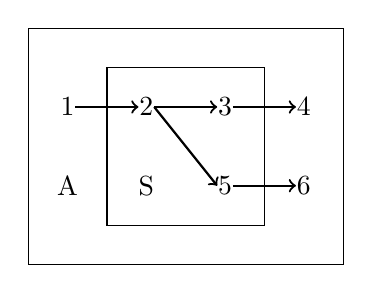
\begin{tikzpicture}
\node at (0,0) {1}; \draw [->,thick] (0.1,0) -- (0.9,0); \node at (1,0) {2}; \draw [->,thick] (1.1,0) -- (1.9,-1); \draw [->,thick] (1.1,0) -- (1.9,0); \node at (2,0) {3}; \draw [->,thick] (2.1,0) -- (2.9,0); \node at (3,0) {4};
\node at (2,-1) {5}; \draw [->,thick] (2.1,-1) -- (2.9,-1); \node at (3,-1) {6};

\draw (0.5,-1.5) rectangle (2.5,0.5); \node at (1,-1) {S};
\draw (-0.5,-2) rectangle (3.5,1); \node at (0,-1) {A};

\end{tikzpicture}

\item $U \circ U = \{(1,3),(1,5),(2,4),(2,6)\}\\
U^3 = U \circ U^2 = \{(1,4),(1,6)\}\\
U^4 = U \circ U^3 = \varnothing \\
\implies U^+ = U \cup U^2 \cup U^3 = ...$

$U^+$ ist asymmetrisch und transitiv, also strikte Ordnung (Skizze \dots \textsc{Hasse} Diagramm

\item
\begin{itemize}
\item $S$ hat keine oberen Schranken, kein Supremum, kein Maximum; aber maximale Elemente: $3,5$
\item untere Schranken $1,2,  \inf{S} = \min{S} = 2$ (=einziges minimales Element)
\end{itemize}
\end{enumerate}

\paragraph{Funktionen}
\subparagraph{Definition 17:} Eine Relation $f\subseteq \mathcal{X} \times \mathcal{Y}$ heißt Funktion (Abbildung) von $\mathcal{X}$ in $\mathcal{Y}$, wenn sie linksvollständig und rechtseindeutig ist.

Diskussion:
\begin{enumerate}
\item Gemäß Definition 7 \ref{def7a} und \ref{def7c} bedeutet linksvollständig und rechtseindeutig, dass zu jedem $x \in \mathcal{X}$ genau ein $y \in \mathcal{Y}$ mit $(x,y) \in f$ existiert, also eindeutige Zuordnung
\[x \rightarrow y =: f(x)\]

Schreibweise
\[ f| \mathcal{X} \rightarrow \mathcal{Y}\]

$y = f(x)$ heißt auch Bild von $x$,
$x$ heißt ein Urbild von $y$ (muss nicht eindeutig sein)
\item $\mathcal{X} =: Db(f)$\dots Definitionsbereich\\
$Wb(f):=\{y\in \mathcal{Y} | \exists x \in \mathcal{X} \quad (x,y) \in f\}$\\
$\subseteq \mathcal{Y}$\dots Wertebereich\\
Schreibweise auch $f(\mathcal{X}):= Wb(f)$
\end{enumerate}

\subparagraph{Definition 18}
\begin{enumerate}
\item Eine Abbildung $f$ heißt surjektiv (auch Abbildung auf $\mathcal{Y}$, wenn $Wb(f)=\mathcal{Y}$
\item Eine Funktion $f$ heißt injektiv (auch umkehrbar, eindeutig oder eineindeutig), wenn es zu jedem $y \in Wb(f)$ genau ein $x \in Db(f)$ existiert mit $(x,y) \in f:$

\[\underbrace{y}_{\in Wb(f)} \longrightarrow \underbrace{x}_{\in Db(f)} =: f^{-1}(y)\]
Die dadurch erklärte Abbildung $f^{-1}| Wb(f) \rightarrow Db(f)$ heißt Umkehrfunktion von $f$, vgl. auch Kapitel 1.4.
\item Eine injektive und surjektive Abbildung heißt bijektiv.
\item Gebräuchlich sind auch die Begriffe Surjektion, Injektion und Bijektion
\end{enumerate}

\subparagraph{Beispiel 12:} Gegeben seien die Mengen $\mathcal{X} = \{ a,b,c\}$ und $\mathcal{Y} = \{1,2,3,4\}$, sowie folgende Relationen in $\mathcal{X} \times \mathcal{Y}:$

\begin{enumerate}
\item $T_1:$\\*
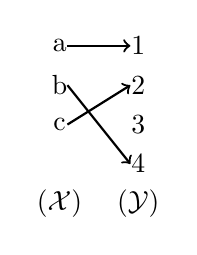
\begin{tikzpicture}[yscale=0.5]
\node at (0,0) {a}; \draw [->,thick] (0.1,0) -- (0.9,0); \node at (1,0) {1};
\node at (0,-1) {b}; \draw [->,thick] (0.1,-1) -- (0.9,-3); \node at (1,-1) {2};
\node at (0,-2) {c}; \draw [->,thick] (0.1,-2) -- (0.9,-1); \node at (1,-2) {3};
\node at (1,-3) {4};
\node at (0,-4) {$(\mathcal{X})$}; \node at (1,-4) {$(\mathcal{Y})$};


\end{tikzpicture}

$T_1$ ist eine Funktion (da linksvollständig und rechtseindeutig), Funktion $f = T_1 :\: f|\mathcal{X} \rightarrow \mathcal{Y}$, diese ist injektiv, $Db(f)=\mathcal{X}, Wb(f) = \{1,2,4\}=:W$

Die Abbildung $f|\mathcal{X} \rightarrow W$ ist auch surjektiv, also bijektiv.
Als Relationen sind $f|\mathcal{X} \rightarrow \mathcal{Y}$ und $f|\mathcal{X} \rightarrow W$ nicht zu unterscheiden, aber als Funktionen.

\item $T_2:$\\*
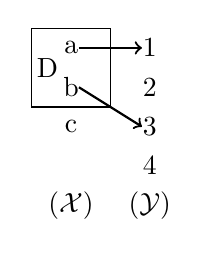
\begin{tikzpicture}[yscale=0.5]
\node at (0,0) {a}; \draw [->,thick] (0.1,0) -- (0.9,0); \node at (1,0) {1};
\node at (0,-1) {b}; \draw [->,thick] (0.1,-1) -- (0.9,-2); \node at (1,-1) {2};
\node at (0,-2) {c}; \node at (1,-2) {3};
\node at (1,-3) {4};
\node at (0,-4) {$(\mathcal{X})$}; \node at (1,-4) {$(\mathcal{Y})$};

\draw (-0.5,0.5) rectangle (0.5,-1.5); \node at (-0.3,-0.5) {D};

\end{tikzpicture}

$T_2$ ist keine Funktion, da nicht linksvollständig. Betrachtetman $D:=\{a,b\}$, so wird durch $T_2$ eine Funktion $f|D\rightarrow \mathcal{Y}$ beschrieben, diese ist injektiv und kann mit $W:= f(D) =Wb(f)=\{1,3\}$ zu einer bijektiven Abbildung $f|D\rightarrow W$ umgewandelt werden.

\item $T_3:$\\*
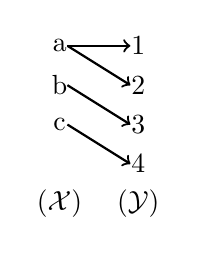
\begin{tikzpicture}[yscale=0.5]
\node at (0,0) {a}; \draw [->,thick] (0.1,0) -- (0.9,0); \draw [->,thick] (0.1,0) -- (0.9,-1); \node at (1,0) {1};
\node at (0,-1) {b}; \draw [->,thick] (0.1,-1) -- (0.9,-2); \node at (1,-1) {2};
\node at (0,-2) {c}; \draw [->,thick] (0.1,-2) -- (0.9,-3); \node at (1,-2) {3};
\node at (1,-3) {4};
\node at (0,-4) {$(\mathcal{X})$}; \node at (1,-4) {$(\mathcal{Y})$};


\end{tikzpicture}


$T_3$ ist keine Funktion, da nicht rechtseindeutig.

\end{enumerate}

\subparagraph{Beispiel 13:}
\begin{enumerate}
\item $f|[0,\infty ) \rightarrow \mathbb{R}$ mit $x\rightarrow y = f(x) = \sqrt{x}$ ist eine Funktion einer reellen Veränderlichen (injektiv, $Db(f)=[0,\infty )$

\item $f| \mathbb{R} \times \mathbb{R} \rightarrow \mathbb{R}$ mit $z=f(x,y)=x^2 +y^2$\\
$(x,y) \rightarrow f(x,y) = x^2 +y^2 =:z$
Funktion zweier reeller Veränderlichen

\item $f|\mathbb{N} \rightarrow \mathbb{R}$ mit $n \rightarrow f(n) = \frac{n}{n+1}$ \dots reelle Zahlenfolge $f(0) = 0, f(1) = \frac{1}{2}, f(2) = \frac{2}{3}, ...$
Bezeichnung meist mit Index $a_n := f(n) \curvearrowright$ Folge $(a_n)_{n \in \mathbb{N}}$
\end{enumerate}


\subparagraph{Definition 19} Es seien $g|\mathcal{X} \rightarrow U$ mit $x \rightarrow u = g(x)$ und $f|U \rightarrow \mathcal{Y}$ mit $u \rightarrow y = f(u)$ zwei Abbildungen. Dann stellt die Zuordnung $x \rightarrow y = f(\underbrace{g(x)}_{u})$ eine Abbildung von $\mathcal{X}$ in $\mathcal{Y}$ dar, eine sogenannte mittelbare Funktion (Komposition/Verkettung).

Bezeichnung: $g \circ f | \mathcal{X} \rightarrow \mathcal{Y}$ mit $y=(g\circ f)(x) = f(g(x))$

Diskussion: 
\begin{enumerate}
\item 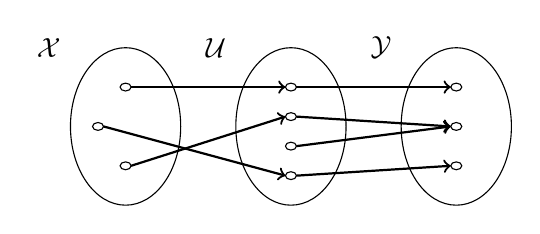
\begin{tikzpicture}[yscale=0.5, xscale=0.7]
%\draw (0,0) grid (2,2);
\node [left] at (-1,2) {$\mathcal{X}$};
\draw (0,0) circle [x radius=1, y radius=2];
\draw (0,1) circle [radius=0.1]; \draw (-0.5,0) circle [radius=0.1]; \draw (0,-1) circle [radius=0.1]; 

\draw [->,thick] (0.1,1) -- (2.9,1);
\draw [->,thick] (-0.4,0) -- (2.9,-1.25);
\draw [->,thick] (0.1,-1) -- (2.9,0.25);

\node [left] at (2,2) {$\mathcal{U}$};
\draw (3,0) circle [x radius=1, y radius=2];
\draw (3,1) circle [radius=0.1]; \draw (3,0.25) circle [radius=0.1]; \draw (3,-0.5) circle [radius=0.1]; \draw (3,-1.25) circle [radius=0.1]; 

\draw [->,thick] (3.1,1) -- (5.9,1);
\draw [->,thick] (3.1,0.25) -- (5.9,0);
\draw [->,thick] (3.1,-0.5) -- (5.9,0);
\draw [->,thick] (3.1,-1.25) -- (5.9,-1);

\node [left] at (5,2) {$\mathcal{Y}$};
\draw (6,0) circle [x radius=1, y radius=2];
\draw (6,1) circle [radius=0.1]; \draw (6,0) circle [radius=0.1]; \draw (6,-1) circle [radius=0.1]; 

\end{tikzpicture}
\begin{align*}
        x \rightarrow u=g(x) &| u\rightarrow y =f(u)=f(g(x))\\
\text{Paarschreibweise} (x,u) \in g &| (u,y) \in f \curvearrowright (x,y) \in g \circ f 
\end{align*}

\item $g$ wird zuerst angewendet, dann $f$; wie bei beliebigen Relationen, also Schreibweise $g \circ f$

\item In der Literatur findet man leider oft die Schreibweise $f \circ g$, offenbar angelehnt an die Schreibweise $f(g(x))$. Die Reihenfolge ist aber von innen nach außen, erst $g$, dann $f$.

\Large{Bei allen späteren Anwendungen von mittelbaren Funktionen (Vorlesungen,Literatur) die Schreibweise überprüfen. Im Zweifelsfall stets die immer eindeutige Schreibweise $f(g(x))$ ohne Verwendung von "`$\circ$"' benutzen!}
\end{enumerate}

\subparagraph{Satz 3} Es sei $f|\mathcal{X} \rightarrow \mathcal{Y}$ eine Bijektion, d.h. es existiert die Umkehrfunktion $f^{-1} | \mathcal{Y} \rightarrow \mathcal{X}$. 
Weiter bezeichne für eine beliebige Menge $A$ die Schreibweise $i_A$ die identische Abbildung (Identitätsrelation, d.h. $i_A | A \rightarrow A$ und $i_A(x)=x \, (x \in A)$.

Es gilt dann:
\[f\circ f^{-1} = i_{\mathcal{X}}, \text{d.h.} (f \circ f^{-1})(x) = f^{-1}(f(x))=x \quad (\forall x \in \mathcal{X} )\]
\[f^{-1} \circ f = i_{\mathcal{Y}}, \text{d.h.} (f^{-1} \circ f)(y) = f(f^{-1}(y))=y \quad (\forall y \in \mathcal{Y} )\]
(Funktion und Umkehrfunktion nacheinander angewandt "`heben sich auf"')

Beweis: ÜA 1.31

\subparagraph{Satz 4} Es seien $g|\mathcal{X} \rightarrow U$ und $h|U\rightarrow \mathcal{Y}$ zwei Bijektionen. Dann ist die Komposition $f:= g\circ h | \mathcal{X} \rightarrow \mathcal{Y}$ ebenfalls eine Bijektion und es gilt:
\[f^{-1}=(g\circ h)^{-1} = h^{-1} \circ g^{-1} \]

Zum Beweis: $x \rightarrow u=g(x) \rightarrow y=h(u) = h(g(x)) = (g \circ h)(x)$\\
Umkehrung: $y\rightarrow u = h^{-1}(y) \rightarrow x=g^{-1}(u) =g^{-1}(h^{-1}(y)) = (h^{-1} \circ g^{-1})(y)$\\
Mehr zu Imkehrfunktionen reeller Funktionen im Kapitel 1.4..

\subsubsection{Gleichmächtigkeit,Kardinalzahlen}
$E$ sei eine (hinreichend umfassende) Grundmenge, die alle für eine mathematische Theorie relevanten Objekte (Zahlen,Funktionen usw.) enthält.

$M$ sei die Potenzmenge von $E$, d.h. $M = \mathcal{P} (E)$

\subparagraph{Definition 20} Zwei Mengen $A$ und $B \quad (A \subseteq E, B\subseteq E \text{bzw.} A \in M, B\in M)$ heißen gleichmächtig.
(Bezeichnung $(A \sim B)$, wenn eine bijektive Abbildung von $A$ auf $B$ (und damit auch von $B$ auf $A$ bzw. zwischen $A$ und $B$) existiert.

Diskussion:

\begin{enumerate}
\item Offensichtlich ist die Relation $T \subseteq M \times M$ mit $(A,B) \in T := A \sim B$ eine Äquivalenzrelation auf $M$.

\item Äquivalenzklassen sind MEngen gleichmächtiger Teilmengen von $E$. Diese Äquivalenzklassen nennt man Kardinalzahlen.
\item Bei endlichen Mengen bedeutet Gleichmächtigkeit: gleiche Anzahl von Elementen.

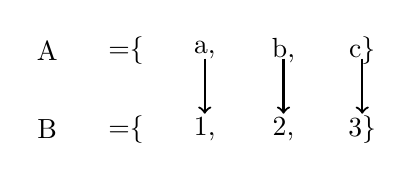
\begin{tikzpicture}

\node at (0,0) {A}; \node at (1,0) {=\{ }; \node at (2,0) {a,}; \node at (3,0) {b,};\node at (4,0) {c\}};

\draw [->,thick] (2,-0.1) -- (2,-0.8);\draw [->,thick] (3,-0.1) -- (3,-0.8);\draw [->,thick] (4,-0.1) -- (4,-0.8);

\node at (0,-1) {B}; \node at (1,-1) {=\{ }; \node at (2,-1) {1,}; \node at (3,-1) {2,};\node at (4,-1) {3\}};

\end{tikzpicture} (bijektive Abbildung)

Bezeichnung: $card\,A = \lvert A \rvert = 3 = \lvert B \rvert$
Natürliche Zahlen sind die Kardinalzahlen endlicher Mengen.

\item Die Anschauung versagt bei unendlichen Mengen.


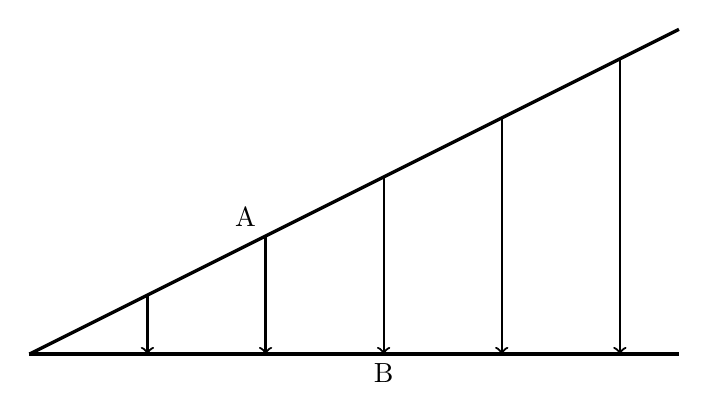
\begin{tikzpicture}[xscale=1.5,yscale=0.75]
%\draw (0,0) grid (5,5);

\node [above left] at (2,2) {A};
\draw [very thick] (0,0) -- (5.5,5.5);

\draw [->,thick] (1,1) -- (1,0); \draw [->,thick] (2,2) -- (2,0); \draw [->,thick] (3,3) -- (3,0); \draw [->,thick] (4,4) -- (4,0); \draw [->,thick] (5,5) -- (5,0); 

\node [below] at (3,0) {B};
\draw [very thick] (0,0) -- (5.5,0);
\end{tikzpicture}

Die Strecken $A$ und $B$ sind gleichmächtig, obwohl A länger als B ist.

\end{enumerate}


\subparagraph{Definition 21} Eine Menge heißt abzählbar unendlich, wenn sie mit der Menge $\mathbb{N} = \{0,1,2,3,...\}$ der natürlichen Zahlen gleichmächtig ist.

Diskussion:
\begin{enumerate}
\item $M$ ist abzählbar unendlich heißt, es existiert eine Zählvorschrift, bei der jedes Element von $M$ nach endlichen vielen Schritten erreicht wird.
\item Die Menge $\mathbb{Z}$ der  ganzen Zahlen ist abzählbar unendlich. 
Anordnung nach wachsenden Betrag: $\mathbb{Z}=\{0,-1,1,-2,2,-3,3,...\}$
\item $\mathbb{Q}^+$ \dots Menge der positiven rationalen Zahlen.
%Todo Optional Foto vom 2013-11-04T16:20

$\mathbb{Q}^+ = \{ \frac{1}{1}, \frac{1}{2}, \frac{2}{1},\frac{1}{3},\xout{\frac{2}{2}},\frac{3}{1}, ...\}$

$\curvearrowright$ Analog zu $\mathbb{Z}$: Die Menge der rationalen Zahlen $\mathbb{Q}$ ist abzählbar unendlich.

\item Es gibt Mengen, die mächtiger als die Menge der natürlichen Zahlen sind: Überabzählbare Mengen.

$B$ heißt mächtiger als $A$, wenn es eine injektive Abbildung $f|A \rightarrow B$ gibt, aber keine bijektive Abbildung, Schreibweise $\lvert A \rvert < \lvert B \rvert$, 

\end{enumerate}

\subparagraph{Satz 5} Die Menge $M=\{ x \in \mathbb{R} |0 < x <1\} = (0;1)$ ist überabzählbar.

Beweis: (\textsc{Cantor}sches Diagonalverfahren): Indirekt, angenommen $M=(0;1)$ sei abzählbar unendlich, d.h. $M=\{ x_1,x_2,x_3,...\} $. Für die Zahlen $x_h$ wählen wir z.B. die eindeutige Darstellung als Dezimalbruch (9er Periode verwenden)\\
$ x_1 = 0,a_1^{(1)} a_2^{(1)} a_3^{(1)} ...$\\
$x_2 = 0,a_1^{(2)} a_2^{(2)} a_3^{(2)} ...$\\
$x_3 = 0,a_1^{(3)} a_2^{(3)} a_3^{(3)} ...$\\
\dots

Es sei $z=0,b_1 b_2 b_3 ...$
mit $b_k =\left\{ \begin{array}{rcl}
         1
         & \mbox{falls}
         & a_k^{(k)} \neq 1 \\ 
         2  
         & \mbox{falls} 
         & a_k^{(k)} = 1 \\
                \end{array}\right. (k=1,2,3,...)$

Damit unterscheiden sich $x_k$ und $z$ auf jedem Fall an der $h$-ten Stelle $\curvearrowright z \neq x_k (\forall k)$, $z$ ist also nicht in der Folge $x_1,x_2,x_3,...$ enthalten, also $z \notin M$. Andererseits gilt $0<z<1$, also $z \in (0;1)=M$ Widerspruch. q.e.d.

\subparagraph{Satz 6} Es sei $E$ eine nichtleere Menge. Dann ist die Potenzmenge $M=\mathcal{P}(E)$ mächtiger als E.

Beweis: 
\begin{enumerate}
\item Die Abbildung $f|E \rightarrow M$ mit $f(x)=\{x\},$ die jedem Element $x \in E$ die eindeutige Teilmenge $\{x\} \in M$ zuordnet ist injektiv.
\item Angenommen, es gäbe eine bijektive damit auch surjektive) Abbildung $g|E \rightarrow M$
Es sei $A=\{x \in E | x \notin g(x)\} \in M$
\end{enumerate}
($A$ ist Teilmenge von $E$). Da $g$ surjektiv ist, gibt es ein Element $a \in E$ mit $g(a) = A$

Fallunterscheidung:\\*
\begin{enumerate}
\item $a\notin A = g(a) \rightarrow a \in A$ (Widerspruch)
\item $a\in A =g(a) \rightarrow a \notin A$ (Widerspruch)
\end{enumerate}
Beide Fälle führen auf Widerspruch, es gibt also keine surjektive Abbildung, damit auch keine bijektive Abbildung von $E$ auf $\mathcal{P}(E).|$

Diskussion: Satz 6 zeigt, dass es unendlich viele unendliche Mächtigkeiten gibt. Zum Beispiel gibt $\lvert \mathbb{N} \rvert < \lvert \mathcal{P} (\mathbb{N}) \rvert < \lvert \mathcal{P} (\mathcal{P} ( \mathbb{N}))\rvert$ usw.

\subparagraph{Satz 7} Die Potenzmenge $\mathcal{P}(\mathbb{N})$ der Menge der natürlichen Zahlen ist gleichmächtig dem Intervall (0;1), also überabzählbar.

Beweis: s ÜA 1.38

\paragraph{Prinzip der vollständigen Induktion} Es sei $n_0 \in \mathbb{N}$.
Zu beweisen ist: "`Für alle natürlichen Zahlen $n\geq n_0$ gilt die Aussage $p(n)$"' Es sind also abzählbar unendlich viele Aussagen zu beweisen.

\subparagraph{Satz 8}
\begin{enumerate}
\item Es sei $p(n_0)$ wahr. (Induktionsanfang)
\item Für alle natürlichen Zahlen $n\geq n_0$ sei die Implikation $p(n) \rightarrow p(n+1)$ wahr (Induktionsschluss)
\end{enumerate}
Dann gilt: $p(n)$ ist für alle $n\geq n_0$ wahr.

Zum Beweis:
\begin{enumerate}
\item $\curvearrowright p(n_0)$ wahr
\item $p(n_0) \rightarrow p(n_0 + 1)$
\end{enumerate}
Prämisse wahr, Implikation wahr $\curvearrowright$ Konklusion $p(n_0 +1 )$ wahr usw.
%%

Beispiel 14: Zu beweisen ist 
\[ \sum\limits_{k=1}^{n} k^2 = \frac{n(n + 1)(2n + 1)}{6} \text{ für alle } n\in N^*\]
\begin{enumerate}
\item $p(1): 1^2 = \frac{1\cdot 2\cdot 3}{6}$ (wahr) Induktionsanfang
\item Es gelte $p(n): \sum\limits_{k=1}^{n} k^2 = \frac{n(n + 1)(2n + 1)}{6}$
\end{enumerate}
zu zeigen $p(n+1) : \sum\limits_{k=1}^{n+1} k^2 = \frac{(n+1)(n+2)(2n+3)}{6}$

Induktionsschluss: $p(n) \rightarrow p(n+1)$\\
$\sum\limits_{k=1}^{n+1} k^2 = \sum\limits_{k=1}^{n} k^2 + (n+1)^2$\\
$= \frac{n(n+1)(2n+1)}{6} + (n+1)^2$\\
$= \frac{n+1}{6} (n(2n +1) + 6(n+1)) = \frac{n+1}{6} (2n^2 + 7n +6)$\\
$=\frac{n+1}{6} (n+2)(2n+3)|$\\

\subsection{Zahlen}
\subsubsection{Gruppen, Ringe Körper}
\begin{itemize}
\item Geg. sei eine Menge $M$ und eine zweistellige Operation $\circ$ (d.h. Abbildung $M \times M \rightarrow M$),
Bezeichnung $(M,\circ)$, analog bei 2 Operationen $(M,\circ , *)$
\item Die Operation $\circ$ heißt kommutativ, wenn $a \circ b = b \circ a$ und assoziativ, wenn $(a\circ b)\circ c= a \circ (b \circ c)$ für beliebige $a,b,c \in M$ gilt.
\end{itemize}
\subparagraph{Definition 1} $(M,\circ)$ heißt Gruppe, wenn gilt:
\begin{enumerate}
\item Die Operation $\circ$ ist assoziativ
\item Es gibt genau ein neutrales Element $e \in M$ mit $a \circ e = e \circ a = a$ (für alle $a \in M$).
\item Es gibt zu jedem $a \in M$ genau ein inverse Element $a^{-1}$ mit $a^{-1} \circ a = a \circ a^{-1} = e$
\item Eine Gruppe heißt \textsc{Abel}sch , wenn zusätzlich gilt: $\circ$ ist kommutativ
\end{enumerate}

\subparagraph{Definition 2} $(M, \oplus , *)$ heißt Ring, wenn gilt:
\begin{enumerate}
\item $(M,\oplus)$ ist \textsc{Abel}sche Gruppe
\item Die Operation $*$ ist assoziativ
\item Es gelten für beliebige $a,b,c \in M$\\
$a*(b \oplus c) = (a \oplus b ) \oplus (a *c)$\\
$(a \oplus b ) * c = (a * c) \oplus (b*c)$ (Distributivgesetz)\\
Eine Ring heißt kommutativer Ring, wenn gilt
\item $*$ ist kommutativ
\end{enumerate}

\subparagraph{Definition 3} $(M, \oplus , *)$ heißt Körper, wenn gilt:
\begin{enumerate}
\item $(M, \oplus , *)$ ist ein Ring (mit dem neutralen Element 0 für die Operation $\oplus$ )
\item $(M\backslash \{0\}, *)$ ist \textsc{Abel}sche Gruppe mit dem neutralem Element 1 für die Operation $*$
\end{enumerate}

\subsubsection{Zahlentheorie}
\begin{itemize}
\item Eine natürliche Zahl $p>1$, die nur durch $1$ und sich selbst teilbar ist, heißt Primzahl
\item Jede natürliche Zahl $n>1$ ist entweder eine Primzahl oder sie lässt sich als Produkt von Primzahlen schreiben. Diese Primzahlenfaktorzerlegung ist bis auf die Reihenfolge eindeutig.
\end{itemize}
\subparagraph{Definition 4} Zwei natürliche Zahlen heißen teilerfremnd, wenn sie außer $1$ keine gemeinsamen Teiler besitzen.

Es sei $a \in \mathbb{Z}$ und $m \in \mathbb{N}^*$ Dann gibt es eine eindeutige Darstellung der Gestalt
$a=q \cdot m +r$ mit $0\leq r <m$ und $q \in \mathbb{Z}$
Bezeichunungen\\
$m$ \dots Modul\\
$r$ \dots (kleinste nicht neg) Rest modulo $m$\\
$r = mod(a,m)$

Zur Erinnnerung: $a$ und $b$ seien ganze Zahlen, $m \in \mathbb{N}^*$, dann $a \equiv b ( \mod{m})$ [ $a$ kongruent $b$ modulo $m$]
$\Leftrightarrow$ $a$ und $b$ haben den gleichen Rest modulo $m$ $\Leftrightarrow$ $a - b$ ist durch $m$ teilbar. D.h. $\forall k \in \mathbb{Z} \; a-b = k \cdot m$

\subparagraph{Satz 1} Es sei $a \equiv b(\mod{m}),\, c\equiv d(\mod{m}),$ dann gilt:
\[a+c \equiv b+d (\mod{m}) \text{ und } a\cdot c \equiv b \cdot d\]
d.h. in Summen und Produkten darf jede Zahl durch einen beliebigen Vertreter der gleichen Restklasse ersetzt werden

Bemerkung: z.B. Restklasse 1 (modulo 7): $\{...,-20,-13,-6,1,8,15,22,...\}$

Beispiel 1 (Modulo m=6)
\begin{enumerate}
\item $307 + 598 \equiv 1 + (-2) \equiv -1 \equiv 5 (\mod{6})$
\item $307 \cdot 598 \equiv 1 \cdot (-2) \equiv -2 \equiv 4 (\mod{6})$
\item $598^6 \equiv (-2)^6 \equiv 64 \equiv 4 (\mod{6})$
\end{enumerate}

Man wählt aus jeder Restklasse den kleinsten nichtnegativen Vertreter $\curvearrowright$ Menge von Resten modulo m $\{0,1,2,...,m-1\}=:\mathbb{Z}_m$
$\curvearrowright$ Modulare Arithmetik: Operationen $\oplus$ und $\odot$ für Zahlen aus $\mathbb{Z}_m$ erklärbar, indem für das Ergebnis jeweils der kleinste nichtnegative Rest modulo $m$ gewählt wird (vgl. Satz 1). Z.B. für $\mathbb{Z}_7 = \{0,1,2,...,6\} : \: 5 \oplus 6 = 4$ (da $5+6 \equiv 11 \equiv 4 (\mod{7})$) $5 \odot 6 =2$, denn $5\cdot 6 \equiv 30 \equiv 2\mod{7})$\\
Falls keine Verwechslungen zu befürchten sind, werden die üblichen Schreibweisen $+ \text{ und } \cdot$ anstelle $\oplus$ bzw. $\odot$ benutzt.

\subparagraph{Definition 5} Wenn es zum $c \in \mathbb{Z}_m$ eine Zahl $d\in \mathbb{Z}_m$ gibt mit $c \cdot d \equiv 1 (\mod{m})$ (bzw. $ c \odot d =1)$, so heißt $d$ die (multiplikative) modulare Inverse von $c$ in $\mathbb{Z}_m$\\
Bezeichnung: $d=c^{-1}$

Beispiel 2: $c=3 \in \mathbb{Z}_7$, wegen $3 \cdot 5 \equiv 1 ( \mod{7})$ ist in $\mathbb{Z}_7: 3^{-1} = 5$

\subparagraph{Satz 2} Zu $a\in \mathbb{Z}_m,\, a\neq 0$, gibt es genau dann eine modulare Inverse in $\mathbb{Z}_m$, wenn $a$ und $m$ teilerfremd sind.

\subparagraph{Satz 3} Es sei $p$ eine Primzahl. Dann ist $(\mathbb{Z}_p,\oplus,\odot)$ ein Körper.\\*
Bemerkung: Falls $m$ keine Primzahl ist, so ist $(\mathbb{Z}_m,\oplus,\odot)$  nur ein kommutativer Ring.

\subparagraph{\textsc{Euklid}ischer Algorithmus}
\begin{itemize}
\item Verfahren zur Ermittlung des größten gemeinsamen Teilers $t$ zweier positiver natürlicher Zahlen $T=ggT(a,b)$
\item In erweiterter Form bietet der Algorithmus eine Möglichkeit zur Berechnung der modularen Inversen von $a$ zum Modul $m \; (a < m, a \text{ und } m$ teilerfremd).b
\end{itemize}

\subparagraph{Satz 4} (\textsc{Euklid}ischer Algorithmus)\\*
Es seien $a,b \in \mathbb{N}^*,\, a >b$. Man bildet die (endliche) Folge
\[ r_0 := b\, , r_1=\mod{(a,b)}, r_2=\mod{(r_0,r_1)},...\]
\[... r_n=\mod{(r_{n-2},r_{n-1})}\, ,\text{Abbruch falls } r_n=0\]
In diesem Fall gilt
\[ggT(a,b)=r_{n-1}\]
(letzter, nicht verschwindender Rest)

Bezeichnungen: $j$-te Division\\
$r_{j-2}: r_{j-1} = q_j \text{ Rest } r_j \: (j=1,...,n)$ \\
(dabei $r_{-1}=a$)

\subparagraph{Satz 5} (erweiterter \textsc{Euklid}ischer Algorithmus)\\*
Zusätzlich zur Folge $(r_n)$ aus Satz 4 bilde man die Folgen \[x_0 = 0, x_1 =1, x_2 = x_0 - q_2x_1,...,x_j=x_{j-2} - q_j x_{j-1}\]
$(j\leq n-1)$ und
\[y_0=1, y_1=-q_1,y_2=y_0-q_2y_1,...,y_j=y_{j-2}-q_jy_{j-1}\]
$(j\leq n-1)$\\
Dann gilt für alle $j=0,...,n-1: \; r_j=x_j a + y_j\cdot b$
Insbesondere gilt $ggT(a,b)=x_{n-1}a + y_{n-1}b$

Diskussion:
\begin{enumerate}
\item Der Sinn des erweiterten \textsc{Euklid}ischen Alg. besteht darin, in jedem Schritt den Divisionsrest als Linearkombination von $a$ und $b$ mit ganzzahligen Koeffizienten $x$ und $y$ darzustellen:
\[ r = x\cdot a + y\cdot b\]
Der Mechanismus wird am besten im nachfolgendem Beispiel 4 deutlich
\item Sind $c$ und $m$ teilerfremd, $1\leq c < m$, d.h. $ggT(c,m)=1$, so erhält man mit Satz 5 $(a=m,b=c)$ eine Darstellung der Form $1=x\cdot m + y\cdot c \; \curvearrowright \; y\cdot c \equiv 1 (\mod{m})$ und damit $c^{-1} \equiv y (\mod{m})$\\
(Für die modulare Inverse muss eventuell noch der in $\mathbb{Z}_{m-1}$ liegende zu $y$ kongruente Wert ermittelt werden)
\end{enumerate}

Beispiel 3: Man ermittle den größten gemeinsamen Teiler $t$ sowie das kleinste gemeinsame Vielfache $v$ der Zahlen 132 und 84
\begin{itemize}
\item Es genügt der "`einfache"' Algorithmus:\\
\begin{align*}
132&:84&=1 &\text{ Rest } 48\\
84 &: 48 &=1 &\text{ Rest } 36\\
48 &: 36&=1 &\text{ Rest } 12 \curvearrowright t=ggT(132,84)=12\\
36&:12&=3 &\text{ Rest } 0_{\text{ENDE}}\\
\end{align*}

\item $v=\frac{a\cdot b}{t} = \frac{132\cdot 84}{12} = 924$
\end{itemize}

Beispiel 4: Man ermittle die modulare Inverse von $\underbrace{11}_{b}$ zum Modul $\underbrace{25}_{a}$

\subparagraph{\textsc{Euler}sche $\varphi$-Funktion} Satz von \textsc{Euler}
\subparagraph{Definition 6} Es sei $n\in \mathbb{N}^*$. Dann \textsc{Euler}sche $\varphi$-Funktion:
\[\varphi (n):= \text{ Anzahl der zu } n \text{teilerfremden Elemente aus } \{1,2,...,n\}\]

Eigenschaften der $\varphi$-Funktion
\begin{itemize}
\item Es sei $\varphi$ eine Primzahl, dann gilt $\varphi (p)=p-1, \, \varphi (p^k)=p^{k-1}(p-1)$
\item Falls $ggT(m,n)=1$, so gilt $\varphi(m\cdot n)=\varphi (m) \cdot \varphi (n)$\\
Speziell \begin{equation} \label{RSA1} n=p\cdot q; p \text{ und } q \text{ Primzahlen, dann } \varphi (n) = (p-1) (q-1)\end{equation}
\end{itemize}

\subparagraph{Satz 6} (Satz von \textsc{Euler})\\*
Es sei $ggT(a,n)=1$, dann gilt \begin{equation} \label{RSA2} a^{\varphi (n)} \equiv 1 (\mod{n})\end{equation}

\subparagraph{RSA-Verschlüsselung}
\begin{itemize}
\item Die Formeln \ref{RSA1} und \ref{RSA2} bilden die Grundlage für die sogenannte RSA-Verschlüsselung. (\textsc{Rivest, SHARMIR, Adleman 1978})
\item Schlüsselerzeugung
\begin{enumerate}
\item Man wählt (in der Praxis sehr große) Primzahlen $p$ und $q$
\item $n:= p q; \; m:=\varphi (n)=(p-1)(q-1)$
\item $e$ wird so gewählt, dass $ggT(e,m)=1$ ist
\item $d:=e^{-1} (\mod{m})$ (modulare Inverse)
\item $(n,e)$ \dots öffentlicher Schlüssel
\end{enumerate}
$(n,d)$ \dots geheimer Schlüssel (geheim ist nur $d$) $p,q$ und $m$ werden nicht mehr benötigt, bleiben aber geheim!
\item Verschlüsselung: Klartext $a$ teilerfremd zu $n$ verschlüsseln mit $e$, d.h. $b:\equiv a^e (\mod{n})$ bilden $\rightarrow b$ \dots Geheimtext
\item Entschlüsselung: Der Empfänger und Besitzer des geheimen Schlüssels bildet $b^d (\mod{n})$ und erhält $b^d \equiv a (\mod{n})$, denn $b^d\equiv (a^e)^d\equiv a^{ed}\equiv a^{1+k\cdot m} \equiv a^{1+k\varphi (n)} \equiv a\cdot (\underbrace{a^{\varphi (n)}}_{\equiv 1 \text{ wegen } \ref{RSA1}})^k \equiv a (\mod{n})$
\item Praktische Durchführung vgl. ÜA 2.4
\end{itemize}

\subsubsection{Reelle Zahlen}
$\mathbb{R}$ \dots Menge der reellen Zahlen\\
Auf $\mathbb{R}$ existiert eine algebraische Struktur und Ordnungsstruktur.

\paragraph{Algebraische Struktur}
$(\mathbb{R},+,\cdot )$ mit den Operationen $+$ (Addition) und $\cdot $ (Multiplikation) ist ein Körper.

\subparagraph{Definition 7}
\begin{enumerate}
\item $0! :=1; \; n!:= n\cdot (n-1)! \; (n\in \mathbb{N}^*)$\\
rekursive Definition)
\item Sei $\alpha \in \mathbb{R}, k\in \mathbb{N}^*$ dann:\\*
$\binom{\alpha}{0} :=1, \binom{\alpha}{k} := \frac{\alpha}{k} \cdot \binom{\alpha -1}{k-1}$ \dots Binominalkoeffizient "`$\alpha$ über $k$"'

$\binom{\alpha}{k} = \frac{\alpha (\alpha -1) \cdot ... \cdot (\alpha -k +1)}{k!}$
\end{enumerate}

Diskussion
\begin{enumerate}
\item Für $k,n \in \mathbb{N}, \, o\leq k \leq n$ gilt:\\
$\binom{n}{k}=\binom{n}{n-k} = \frac{n!}{k!(n-k)!}$
\item Binomischer Satz
\[(a+b)^n = \sum\limits_{k=0}^{n} \binom{n}{k} a^{n-k} b^k = a^n + \binom{n}{1} a^{n-1} b + \binom{n}{2} a^{n-2} b^2 + ... + b^n\]
\end{enumerate}
\subparagraph{Stellenwertsysteme}
\begin{itemize}
\item Es sei $b>1$ eine natürliche Zahl (die sogenannte Basis)
\item \begin{equation} \label{*} \begin{split}x=(x_p x_{p-1} ... x_1 x_0, x_{-1} x_{-2} ... x_{-q})_b:=
x_p \cdot b^p + x_{p-1} \cdot b^{p-1} + ... \\ + x_1 \cdot b^1 + x_0b^0 + x_{-1} b ^{-1} + ... + x_{-q} b^{-q}\end{split}\end{equation} heißt Darstellung von $x$ zur Basis $b$.
\item Übergang von einem Ziffernsystem zu einem anderen Grundlage: Aus \ref{*} ergibt sich durch fortgesetztes Klammern 
\begin{equation} \label{**}\begin{split}
x=((...((x_pb + x_{p-1}) b + x_{p-2})b+...+ x_2)b +x_1)b + x_0\\ ((...(x_{-q}b^{-1} + x_{-(q-1)})b^{-1} + ... + x_{-2})b^{-1} + x_{-1})b^{–1}\end{split}\end{equation}
\end{itemize}

Beispiel 8:
\begin {enumerate}
\item $(A8C,B2)_{16} = (1010\: 1000\: 1100, 1011\: 0010)_2$
\item $(\underbrace{110}_{6} \underbrace{1110}_{14=E},\underbrace{101(0)}_{10=A})_2 = (6E,A)_{16}$
\end {enumerate}

\paragraph{Zahlendarstellung im Computer}

\subparagraph{Ganze Binärzahlen in Zweierkomplementdarstellung}
($n$ Bit, mit n=8,16,32,64)

\begin{itemize}
\item Beispiel: $n=8 : (100)_{10} = (64)_{16}$\\
$01100100$\\
$\underbrace{2^7}_{\text{MSB}} 2^6 2^52^42^32^22^1\underbrace{2^0}_{\text{LSB}}$

%Todo Wertetablle richtig machen (siehe Foto 2013-11-18T15:23)

MSB\dots most significant bit\\*
LSB\dots least siginificant bit
\item Um auch negative Zahlen darstellen zu können, wird das MSB als Vorzeichenbit reserviert. Negative zahlen $-a \; (1\leq a \leq 2^{n-1})$ werden im sogenannten Zweierkomplement $\bar{a} := 2^n -a \quad (\curvearrowright \bar{a} \leq 2^{n-1} \curvearrowright \text{MSB}=1)$
\item Nichtnegative Zahlen $0\leq a \leq 2^{n-1} -1$ werden unverändert dargestellt. $(\text{MSB}=0)$
\item Damit Darstellung ganzer Zahlen von $-2^{n-1}$ bis $2^{n-1} -1$
\end{itemize}

\subparagraph{Umwandlung negativer Zahlen in Zweierkomplement}
Beispiel 9: $(n=8)$ umzuwandeln sei $-100 (dezimal)$

\begin{enumerate}
\item Möglichkeit (für die Handrechnung):\\
$\overline{100} = \underbrace{2^8}_{256} - 100 = \underbrace{156}_{(9C)_{16}} = 10011100$%Todo Pfeil auf MSB mit "$\text{MSB} = 1 \curverarrowright$ Zahl ist negativ

Bemerkung: Das Zweierkomplement der positiven Zahl $100$ ist die positive Zahl $\overline{100}=156$, diese wird wegen $\text{MSB}=1$ als negative Zahl $-100$ interpretiert.
\item Möglichkeit (am schnellsten!)
Rechts (bzw. LSB) beginnend alle Ziffern bis einschließlich der ersten 1 unverändert lassen, für alle höherwertigen Ziffern $z$ das Einerkomplement $1-z$ bilden.\\
$100:0110 \: 0100$\\*
$\overline{100}: 1001\:1100$
\end{enumerate}

Rückumwandlung (Zahl ist mit $\text{MSB}=1 \rightarrow$ negative Zahl) analog $\overline{156} = 256 -156=100 \curvearrowright -100$\\
Die Subtraktion wird auf die Addition des Zweierkomplements zurückgeführt.

Beispiel 10: $a=64-100=64+(-100)$


Bemerkung: Für die Handrechnung (z.B.) $2-5=:a$) kleinere Zahl von der größeren Subtrahieren $a=-(5-2)$, daher genügt für $n$ die Binärstellenzahl des Minuenden $(5)_{10} = (101)_2$, also $n=3$.\\
Es wird ausschließlich mit nichtnegativen Zahlen gerechnet:\\* $(5-2)_{10} = ((5+\underbrace{2^n -2}_{\bar{2}}) -2^n)_{10} = (5+\bar{2} - 2^n)_{10}$\\
$2=(010)_2 \curvearrowright \bar{2} = (110)_2$\\
$5          101 +$\\*%Todo 101 und 110 und 011 in Kasten
$\bar{2}    110$\\*
$(1) 011$ vordere Stelle ignorieren ($2^n$)\\
$\curvearrowright 5-2 =3 \curvearrowright a=-3$

Verallgemeinerung: Festkommasystem (feste Stellenzahl, Komma an fester Stelle).\\
Vorteil: rundungsfreie Rechnung, nur Überlauf \footnote{
Ein Überlauf (Ergebnis $\geq 2^{n-1}$ oder $< -2^{n-1}$) entsteht in folgenden Fällen \textsc{Error}:
\begin{tabular}{c|c|c|c}
&a&b&$a+b$  \\ \hline
MSB&0&0&1\\ \hline
MSB&1&1&0\\
\end{tabular}
} muss beachtet werden\\

Nachteil: Nur sehr beschränkter Zahlenbereich darstellbar $\rightarrow$ 

\subparagraph{Gleitkommasystem}
\[x=v\cdot m \cdot b^e\]
\begin{itemize}
\item $v=(-1)^V$ \dots Vorzeichen $=\left\{ \begin{array}{rl}
         V=0
         & \mbox{positive Zahl}\\ 
         V=1  
         & \mbox{negative Zahl} \\
                \end{array}\right.$
                
\item $m$ \dots Mantisse, Stellenzahl $p$, die Mantisse heißt normalisiert, falls sie die Gestalt $m_1,m_2m_3 ... m_p$ oder $0,m_1 m_2 ... m_p$ mit $m_1 \neq 0$, dabei $m_1,...,m_p$ Ziffern zur Basis $b$
\item $e$ \dots Exponent, ganzzahlig $e_{min} \leq e \leq e_{max}$

\end{itemize}

In jedem Gleitkommasystem sind nur endlich viele Zahlen darstellbar, Die Menge der reellen Zahlen ist aber überabzählbar (unendlich). Gleitkommazahlen liegen auf der reellen Zahlenachse diskret verteilt (fester Exponent $\curvearrowright$ gleiche Abstände, wächst der Exponent um $k$, so wachsen die Abstände auf das $b^k$-fache)\\
Veranschaulichung für $b=10$, Mantissenlänge $p=1$

Rundung: Zahlen die nicht in dieses "`Raster"' passen, werden auf die nächstgelegene Gleitkommazahl gerundet.\\
Falls die Zahl genau in der Mitte zwischen zwei "`Rasterzahlen"' liegt, wird auf die nächstgelegene gerade Zahl gerundet.

\subparagraph{Numerische Probleme beim Rechnen mit Gleitkommazahlen}
\begin{itemize}
\item Kommutativ-, Assoziativ- und Distributivgesetze gelten allgemein nicht. Ursachen sind z.B. Ziffernauslöschung bei Subtraktion von fast gleichen Zahlen, Addition oder Subtraktion von Zahlen unterschiedlicher Größenordnung, Aufsummierung von Rundungsfehlern.
\item Beispiel 11:
Man berechne $(a+b)+c$ und $a+(b+c)$ in einem System mit 3-stelliger Mantisse:\\
$a=3,73 \cdot 10^6, b= -3,71 \cdot 10^6, c=6,42\cdot 10^3$\\
$a+b = 0,02\cdot 10^6=2,00\cdot 10^4$ (Normalisierung) $c=6,42\cdot 10^3 = 0,642 \cdot 10^4 = 0,64\cdot 10^4$ (Exponentenausgleichung und Rundung).\\
$\curvearrowright (a+b) +c =2,64\cdot 10^4 = \underline{\underline{26400}}$\\
$c=0,00642 \cdot 10^6 = 0,01 \cdot 10^6$ (Exponentenausgleichung und Rundung)\\
$\curvearrowright b+c=-3,70\cdot 10^6$\\
$\curvearrowright a+(b+c) = 0,03 \cdot 10^6 = 3,00\cdot 10^4 = \underline{\underline{30 000}}$\\
exakter Wert: $a+b+c=\underline{\underline{26420}}$
\item Aufgabe der numerischen Mathematik ist es, die unvermeidlichen Genauigkeitsverluste beim Rechnen mit Maschinenzahlen durch optimale Organisation der Rechnung und Fehleranalyse in Grenzen zu halten.

\end{itemize}

\paragraph{Gleitkommaformel IEEE 754} (single precision, 32 Bit)
\[x=v\cdot m \cdot b^e = (-1)^V \cdot 1, m_2m_3 \cdot ... \cdot m_{24} \cdot 2^{E-B} (b=2)\]
\begin{itemize}
\item Vorzeichen $V=0 \curvearrowright$ positiv, $V=1 \curvearrowright$ negativ (1Bit)
\item Mantisse $m_1$ im Binärsystem stets $=1 \curvearrowright$ nur Abspeicherung von $M=m_2m_3 \dots m_{24}$ (23 Bit)
\item Exponent Abgespeichert wird $E:= e+B$, (mit dem sogenannten Biaswert $B=127$) als nichtnegative 8-stellige Binärzahl, (8 Bit)\\
$e_{min} = -126 (E=1), e_{max} = 127 (E=254=1111 \, 1110)_2)$\\
(Die Grenzfälle $E=(0000 \, 0000)_2$ und $E=(1111 \, 1111)_2$ sind für Sonderfälle vorgesehen $(0,\infty ,$ nicht definierte Werte))
\item Abspeicherung in der Reihenfolge $V| E |M$

\end{itemize}

\subparagraph{Beispiel 12} Umwandlung Dezimalzahl IEEE 754 (32-Bit) $x=435,9$ (vgl. Beispiel 6)

\begin{enumerate}
\item Konvertierung in Dezimalzahl (unter Verwendung von Beispiel 6 /Hexadezimalzahl)\\
\[x=(1 \underbrace{B}_{11} 3, \underbrace{E}_{14} \bar{6})_{16} = (1 \, 1011 \, 0011, 1110 \, \underbrace{0110}_{\text{Periode}} \, \underbrace{0110} \, \underbrace{...})_2\]

\item Normalisierte Darstellung, Mantisse mit 23 Stellen nach Komma $\curvearrowright$
\[x=(1, \underbrace{ 1011 \, 0011 \, 1110 \, 0110 \, 0110 \, 011}_{M \text{ (Abrundung!)}}|0 \, 0110 \, ...)_2 \cdot 2^8\]
\item Exponent $e=8 \curvearrowright E=e+B=8+127=135=(87)_{16} = (1000 \, 0111)_2$
\item $V=0$ (da $x$ positiv)\\
$\curvearrowright x \cdot 0| \, 1000 \, 0111 |\, 1011 \, 0011 \, 1110 \, 0110 \, 0110 \, 011$ %Todo Box
\end{enumerate}

\subparagraph{Beispiel 13} IEEE754 Dezimalzahl\\
$1| \, 1000 \, 0011|\, 0111 \, 1100 \, 0000 \, 0000 \, 0000 \, 000$
\begin{enumerate}
\item $E=(1000 \, 0011)_2 = 131 \curvearrowright e=E-B = 131 - 127=4$
\item $V=1 \curvearrowright x < 0$, normalisierte Mantisse $1,M$\\
$\curvearrowright \underline{x} = -(1,\, 0111 \, 11)_2 \cdot 2^4= -(1 \, 0111, 11)_2 = \underline{\underline{-23,75}}$
\end{enumerate}

Bemerkungen:
\begin{enumerate}
\item Neben dem single Format gibt es in IEEE 754 u.a. das double Format (64 Bit , V=1 Bit, E=11 Bit, M=52 Bit, $B=2^{10} -1 = 1023$)
\item Zahlenbereiche:\\*
single: $1,401 \cdot 10^{-45} ... 3,403 \cdot 10^{38}$\\*
double: $4,941 \cdot 10^{-324} ... 1,798 \cdot 10^{308}$
\end{enumerate}

\paragraph{Ordnungsstrutkur}
\begin{itemize}
\item Durch $\leq$ ist auf $\mathbb{R}$ eine vollständige Ordnungsrelation erklärt.
\item Verträglichkeit mit der algebraischen Struktur: $\forall x,y,z \in \mathbb{R}:$\\*
\begin{enumerate}
\item $x \leq y \Rightarrow x + z \leq y + z$
\item $(x \leq y) \wedge (z \geq 0) \Rightarrow x \cdot z \leq y \cdot z$
\item $(x \leq y) \wedge (z \leq 0 ) \Rightarrow x \cdot z \geq y \cdot z$

\end{enumerate}
\end{itemize}

\subparagraph{Definition 8} Es sei $x$ eine reelle Zahl. Dann heißt $\lvert x \rvert := \left\{ \begin{array}{rcl}
         x
         & \mbox{falls}
         & x\geq 0\\ 
         -x  
         & \mbox{falls}
         & x < 0 \\
                \end{array}\right.$
der (absolute) Betrag von $x$.\\
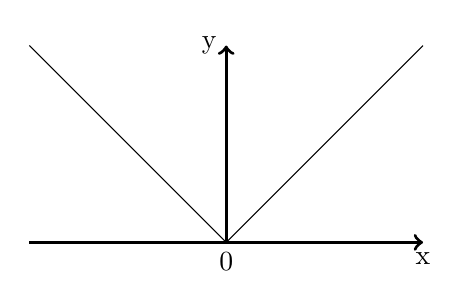
\begin{tikzpicture}[yscale=0.5, xscale=0.5]
\draw [->,very thick] (0,0) -- (0,5); \node [left] at (0,5) {y};
\draw [->,very thick] (-5,0) -- (5,0); \node [below] at (5,0) {x};

\node [below] at (0,0) {0}; 

\draw [domain=-5:5] plot (\x, {abs(\x)});

\end{tikzpicture}

Diskussion: Es gilt
$\lvert a-b \rvert =$ "`Abstand der Zahlen $a$ und $b$ auf der Zahlengeraden"'\\
\begin{tikzpicture}
\draw [->,thick] (0,0) -- (10,0);
\node [below] at (4,0) {a}; \draw [thick] (4,-0.1) -- (4,0.1);
\node [below] at (7,0) {b}; \draw [thick] (7,-0.1) -- (7,0.1);

\draw [help lines] (4,0) -- (4,1);
\draw [<->] (4,1) -- (7,1); \node [above] at (5.5,1) {$\lvert a - b \rvert$};
\draw [help lines] (7,0) -- (7,1);

\end{tikzpicture}

Speziell $\lvert a \rvert$ \dots "`Abstand von $a$ zum Ursprung $0$"'

Lösen von Ungleichungen\\
Beispiel 14 (Ungleichung von Beträgen)\\
Gesucht Lösungsmenge $L$ der reellen Zahlen, die die Ungleichung
\begin{equation}\label{Bsp14*}
\lvert x-1 \rvert < 3 + \frac{1}{2} \cdot x
\end{equation}
erfüllen.
\begin{itemize}
\item "'kritische"` Stellen: Nullstelle des Terms innerhalb der Betragszeichen, also $x=1$\\
$\curvearrowright$ Fallunterscheidung\\
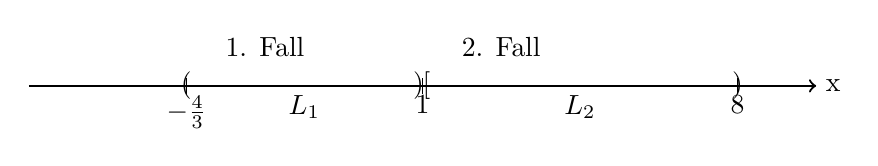
\begin{tikzpicture}
\draw [->,thick] (0,0) -- (10,0);

\node  at (3,0.5) {1. Fall};
\node  at (6,0.5) {2. Fall};
\node [below] at (5,0) {1}; \draw (5,-0.1) -- (5,0.1);
\node [right] at (10,0) {x};

\node at (2,0) {(}; \node [below] at (2,0) {$-\frac{4}{3}$}; \draw (2,-0.1) -- (2,0.1);
\node [below] at (3.5,0) {$L_1$}; \node at (4.95,0) {)};

\node at (5.05,0) {[}; \node at (9,0) {)}; \node [below] at (9,0) {8}; \draw (9,-0.1) -- (9,0.1); \node [below] at (7,0) {$L_2$};

\end{tikzpicture}\\
Dabei jeweils Beträge auflösen gemäß Definition 8


\item 1. Fall 
\begin{align*}
x<1, \quad (\ref{Bsp14*}) &\Leftrightarrow -(x-1) < 3 + \frac{1}{2} x\\
\text{d.h. } x-1<0 \quad &\Leftrightarrow -\frac{3}{2} x < 2 \quad |: (-\frac{3}{2})\\
&\Leftrightarrow \underline{\underline{x > -\frac{4}{3}}}
\end{align*}
$\curvearrowright L_1=\{x|x<1 \wedge x > -\frac{4}{3} \} = \underline{\underline{(-\frac{4}{3};1)}}$

\item 2. Fall
\begin{align*}
x \geq 1, \quad (\ref{Bsp14*}) &\Leftrightarrow (x-1) < 3 + \frac{1}{2} x\\
&\Leftrightarrow \frac{1}{2}x < 4 \quad |:\frac{1}{2}\\
&\Leftrightarrow x < 8
\end{align*}
$\curvearrowright L_2 = \{ x | x\geq 1 \wedge x < 8 \} = \underline{\underline{[1;8)}}$\\
$\curvearrowright L = L_1 \cup L_2 = \underline{\underline{(-\frac{4}{3},8)}}$
\end{itemize}

\subparagraph{Beispiel 15} (Ungleichungen mit gebrochen rationalen Termen)
\begin{equation}\label{Bsp15*}
\frac{x}{x+1} < 1 \quad |\cdot (x+1)
\end{equation}
\begin{itemize}
\item Falls $x+1 <0$ kehrt sich Ungleichungszeichen um! $\curvearrowright$ Fallunterscheidung
\item kritische Stelle(n): Nenner-Nullstellen, hier $x=-1$
\item 1. Fall: $x<-1 \quad (\ref{Bsp15*}) \Leftrightarrow x > x+1 \Leftrightarrow 0 > 1 \quad \curvearrowright$ Widerspruch\\
$x+1 < 0$\\
$\curvearrowright \underline{\underline{L_1 = \varnothing}}$

\item 2. Fall: $x > -1 \quad (\ref{Bsp15*}) \Leftrightarrow x < x+1 \Leftrightarrow 0 < 1$ (wahre Aussage)\\
$\curvearrowright L_1=\{ x | x > -1\wedge 0 < 1 \} = \underline{\underline{(-1;\infty)}}$\\
$\curvearrowright L = L_1 \cup L_2 = \underline{\underline{(-1;\infty)}}$ 
\end{itemize}

\subparagraph{Beispiel 16} (quadratische Ungleichungen)
\begin{align*}
x^2 + 3x < 10 &\Leftrightarrow (x+\frac{3}{2} )^2 - \frac{9}{4} < 10\\
&\Leftrightarrow (x + \frac{3}{2} )^2 < \frac{49}{4}\\
&\Leftrightarrow \lvert x + \frac{3}{2} \rvert < \frac{7}{2}\\
&\Leftrightarrow -\frac{7}{2} < x + \frac{3}{2} < \frac{7}{2}\\
&\Leftrightarrow \underline{\underline{-5 < x < 2}}
\end{align*}

Diskussion:
\begin{itemize}
\item In vielen Fällen ist auch ein grapischer Lösungsansatz möglich. Dabei sind geeignete Schnittpunkte (= Gleichung) exakt rechnerisch zu ermitteln, anschließend Ungleichungszeichen betrachten.
\item Im Beispiel 16: $x^2 + 3x < 10 \Leftrightarrow \underbrace{x^2 + 3x -10}_{=: f(x)} < 0$\\
Nullstellen von $f(x): x^2 + 3x -10 = 0 \curvearrowright x_1 = -5, \, x_2 = 2$\\
\begin{tikzpicture}[yscale=0.125, xscale = 0.5]
\draw [->,thick] (-6,0) -- (6,0); \node [below] at (6,0) {x};
\draw [->,thick] (0,-10) -- (0,25); \node [left] at (0,25) {y};
\draw [domain=-7:4] plot (\x, \x * \x + 3 * \x - 10);
\draw [<->, ultra thick] (-5,0) -- (2,0);
\node [below] at (-5,0) {$-5$}; \node [below] at (2,0) {$2$};
\draw (-5,-0.1) -- (-5,0.1); \draw (2,-0.1) -- (2,0.1);
\node [above] at (-1.5,0) {$L$};
\end{tikzpicture}\\
$\curvearrowright L=(-5;2)$

\end{itemize}

\subparagraph{Schranken und Grenzen}
\begin{itemize}
\item Eine Menge $M \subseteq \mathbb{R}$ heißt nach oben beschränkt, wenn es eine obere Schranke gibt, vgl. Kapitel 1.2..\\ Man kann zeigen, dass es bei dieser Ordnungsrelation $(\leq )$ auf $\mathbb{R}$ dann auch eine kleinste obere Schranke $s$ gibt.\\
(= Supremum $\sup{M}; s=\max{M} \text{ falls } s \in M)$
\item Analog: nach oben beschränkt, Infimum, Maximum
\item Falls $M$ nicht nach oben beschränkt ist, d.h. falls gilt:\\*
$\exists a \in \mathbb{R} \forall x \in M \; x \leq a \equiv \forall a \in \mathbb{R} \exists x \in M \; x > a,$ dann\\
Schreibweise $\sup{M} := \infty$
\item Analog: $\inf{M} = - \infty$
\item $M$ heißt beschränkt, falls $M$ nach oben und unten beschränkt ist.
\end{itemize}

\subparagraph{Beispiel 17} $M= \{ 1 + \frac{1}{n} | n \in \mathbb{N}^*\}$
\begin{itemize}
\item obere Schranken z.B: $3712; \pi ; 2,01$\\
kleinste obere Schranke $\sup{M}=\max{M}=2$
\item untere Schranken: z.B: $-31; 0;0,99$\\
größte untere Schranke $\inf{M}=1$\\*
$1 \notin M \curvearrowright \min{M}$ existiert nicht!
\end{itemize}

\subsubsection{Komplexe Zahlen}
Motivation: z.B. $x^2 = -1$ im Bereich der reellen Zahlen nicht lösbar $\curvearrowright$ Zahlenbereichserweiterung

\paragraph{Begriff, Rechenregeln} 
Die Menge $\mathbb{C}$ der komplexen Zahlen ist eine Obermenge der Menge der reellen Zahlen mit folgenden Eigenschaften:
\begin{enumerate}
\item $\mathbb{C}$ enthält eine Zahl $i$ mit $i^2 = -1$ (oft auch $j$ bezeichnet)
\item Jede komplexe Zahl $z$ lässt sich in der Form $z = x + i \cdot y \quad (x,y \in \mathbb{R})$ darstellen.\\
Dabei
\begin{align*}
x &= Re(z) \text{ \dots Realteil}\\
y &= Im(z) \text{ \dots Imaginärteil}
\end{align*}
\item Auf $\mathbb{C}$ werden die Operatoren $+$ (Addition) und $\cdot$ (Multiplikation) wie folgt erklärt:\\
Es seien $z_1 = x_1 + i y_1, \, z_2 = x_2 + i y_2$

Dann:\\ 
$z_1 + z_2 := x_1 + x_2 + i (y_1 + y_2)$\\*
$z_1 \cdot z_2 := x_1 \cdot x_2 - y_1 y_2 + i (x_1 y_2 + x_2 y_1)$

Die Menge $\mathbb{C}$ wird mit diesen Operationen zum Körper der komplexen Zahlen. Die arithmetischen Operationen erfolgen unter Beachtung von $i^2 = -1$ wie im Reellen.

\item Auf $\mathbb{C}$ gibt es keine natürliche Ordnungsrelation.
\end{enumerate}

Veranschaulichung: \textsc{Gauss}sche Zahlenebene\\
Zahl $z \leftrightarrow \text{ Punkt } P(x,y) \leftrightarrow \overrightarrow{OP}$ (Vector)\\
\begin{tikzpicture}
\draw [->,thick] (0,-5) -- (0,5); \node [left] at (0,5) {imaginäre Achse}; \node [left] at (0,1) {$i$}; \node [above] at (1,0) {$1$}; \node [below left] at (0,0) {$0$};
\draw [thick] (1,-0.1) -- (1,0.1);
\draw [thick] (-0.1,1) -- (0.1,1);
\draw [->,thick] (-1,0) -- (5,0); \node [below] at (6,0) {reelle Achse}; 

\draw (4,4) circle [radius=0.1]; \draw [->,very thick] (0,0) -- (4,4); \node [above] at (4,4) {$P$}; \node [right] at (4,4) {$z=x + iy$};
\node [above] at (2,2) {$\lvert z\rvert$};

\draw [->,thick] (1.5,0) arc [radius= 1.5, start angle = 0, end angle = 45]; \node [right] at (1.5,0.5) {$\varphi$};

\draw [->] (0,0) -- (4,-4);  \node [right] at (4,-4) {$\bar{z}=x - iy$}; \node [below] at (2,-2) {$\lvert z\rvert$};

\node [left] at (0,4) {$iy$}; \draw [help lines] (0,4) -- (4,4);
\node [left] at (0,-4) {$-iy$}; \draw [help lines] (0,-4) -- (4,-4);

\node [below] at (4,0) {$x$}; \draw [help lines] (4,-4) -- (4,4);

\end{tikzpicture}

\begin{itemize}
\item Betrag von $z : \: \lvert z \rvert = \sqrt{x^2 + y^2}$
\item Hauptargument von $z$: orientierter Winkel $\varphi $ von positiver x-Achse zum Strahl $\overrightarrow{OP}$ (gemessen auf kürzestem Wege!)\\
$\curvearrowright Arg \, z := \varphi (-\pi < \varphi \leq \pi )$
\item $\bar{z} = x - iy$ \dots die zu $z = x + iy$ konjugiert komplexe Zahl.
\end{itemize}

Diskussion:
\begin{enumerate}
\item Falls nicht notwendig kürzester Weg gewählt wird $\rightarrow$ Argument $arg \, z = Arg \, z + 2k\pi , \; k \in \mathbb{Z}$

z.B: $z=1-i$\\*
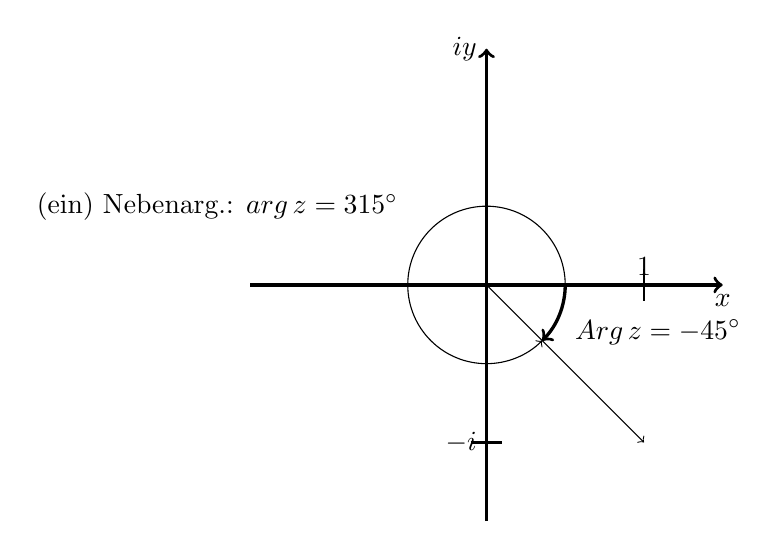
\begin{tikzpicture}[scale=2]
\draw [->,very thick] (-1.5,0) -- (1.5,0); \node [below] at (1.5,0) {$x$};
\draw [->,very thick] (0,-1.5) -- (0,1.5); \node [left] at (0,1.5) {$iy$};
\draw [thick] (1,-0.1) -- (1,0.1);
\draw [thick] (-0.1,-1) -- (0.1,-1);
\node [left] at (0,-1) {$-i$}; \node [above] at (1,0) {$1$};
\draw [->] (0,0) -- (1,-1);

\draw [->,very thick] (0.5,0) arc [radius=0.5, start angle=0, end angle= -45 ]; \node [right] at (0.5,-0.3) {$Arg \, z = -45^{\circ}$};

\draw [->] (0.5,0) arc [radius = 0.5, start angle =0, end angle =315]; \node [left] at (-0.5,0.5) {(ein) Nebenarg.: $arg \, z =315^{\circ}$};

\end{tikzpicture}

\item Berechnung von $Arg \, z (z\neq 0): \; \cos{\varphi} = \frac{x}{\lvert x \rvert} \curvearrowright$

\[ 
Arg \, z =\left\{ \begin{array}{rcl}
         \arccos(\frac{x}{\lvert z \rvert})
         & \mbox{falls}
         & y \geq 0 \\ 
         - \arccos(\frac{x}{\lvert z \rvert})  
         & \mbox{falls} 
         & y <0 \\
                \end{array}\right.
\]
\end{enumerate}

Beispiel 18: $z_1 = 3+4i, \, z_2 = -12 -5i$
\begin{enumerate}
\item Betrag u. Hauptargument
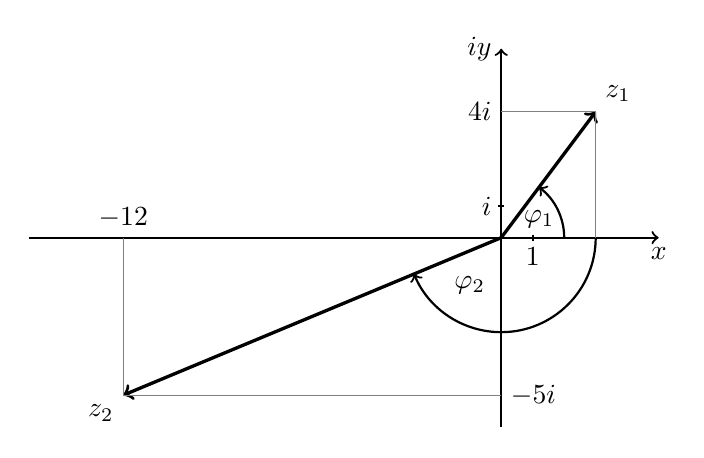
\begin{tikzpicture}[scale=0.4]
\draw [->,thick] (-15,0) -- (5,0); \node [below] at (5,0) {$x$};
\draw [->,thick] (0,-6) -- (0,6); \node [left] at (0,6) {$iy$};

\node [left] at (0,1) {$i$}; \node [below] at (1,0) {$1$};
\draw [thick] (1,-0.1) -- (1,0.1);
\draw [thick] (-0.1,1) -- (0.1,1);

\draw [->,very thick] (0,0) -- (3,4); \node [above right] at (3,4) {$z_1$}; \draw [->,thick] (2,0) arc [radius=2, start angle=0, end angle= 53.13]; \node [above] at (1.2,0) {$\varphi_1$};

\draw [->,very thick] (0,0) -- (-12,-5); \node [below left] at (-12,-5) {$z_2$}; \draw [->,thick] (3,0) arc [radius=3, start angle=0, end angle= -157.38]; \node at (-1,-1.5) {$\varphi_2$};

\draw [help lines] (3,0) -- (3,4); \draw [help lines] (0,4) -- (3,4); 
\draw [help lines] (-12,0) -- (-12,-5); \draw [help lines] (0,-5) -- (-12,-5);

\node [above] at (-12,0) {$-12$}; %\node [above] at (3,0) {$3$};
\node [left] at (0,4) {$4i$}; \node [right] at (0,-5) {$-5i$};

\end{tikzpicture}

$\lvert z_1 \rvert = \sqrt{3^2 + 4^2} = 5$\\
$\varphi_1 = Arg \, z_1 = \arccos{\frac{3}{5}} = \underbrace{53,13^\circ}_{\text{Gradmaß=DEG}}$\\
$\lvert z_2 \rvert = \sqrt{(-12)^2 + (-5)^2} = 13$\\
$\varphi_2 = Arg\, z_2 = - \arccos{\frac{-12}{13}} = -157,38^\circ$

\item Arithmetische Operationen\\
Addition: $z_1 + z_2 = -9 -i$\\
Subtraktion: $z_1 - z_2 = 15 + 9i$\\
Multiplikation: $z_1 \cdot z_2 = -36 -15i -48i -20\underbrace{i^2}_{-1} = -16 -63i$\\
Division: $\frac{z_1}{z_2} = \frac{z_1}{z_2} \cdot \frac{\bar{z_2}}{\bar{z_2}}$ (Erweiterung mit $\bar{z_2} \curvearrowright$ Nummer wird reell $z_2 \cdot \bar{z_2} = \lvert z_2 \rvert^2$)\\
also: $\frac{z_1}{z_2} = \frac{3+4i}{-12-5i} \cdot \frac{-12 +5i}{-12+5i}=-\frac{56}{169} - \frac{33}{169}i$
\end{enumerate}

\paragraph{Trigonometrische Darstellung}\textsc{Euler}sche Formel, exponentielle Darstellung\\
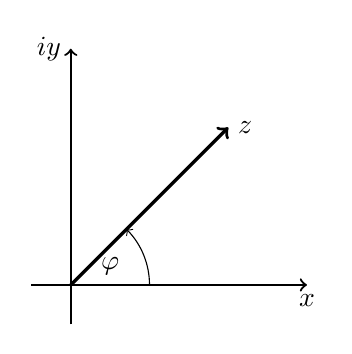
\begin{tikzpicture}
\draw [->,thick] (-0.5,0) -- (3,0); \node [below] at (3,0) {$x$};
\draw [->,thick] (0,-0.5) -- (0,3); \node [left] at (0,3) {$iy$};

\draw [->,very thick] (0,0) -- (2,2); \node [right] at (2,2){$z$};
\draw [->] (1,0) arc [radius=1, start angle=0, end angle=45]; \node [above] at (0.5,0){$\varphi$};

\end{tikzpicture} (mit $\varphi = arg\, z$ meist $\varphi = Arg\, z$)\\
$x=\lvert z\rvert \cos{\varphi}$\\*%}
$y=\lvert z \rvert \sup{\varphi}$%} Todo $z=x+iy$ (arithmetische Darstellung)

$z=\lvert z \rvert (\cos{\varphi} + i \sin{\varphi})$ (trigonometrische Darstellung.

Diskussion: $z_1 = \lvert z_1 \rvert (\cos{\varphi_1} + i \sin{\varphi_1}), z_2 = \lvert z_2 \rvert (\cos{\varphi_2} + i \in{\varphi_2})$\\*
$\curvearrowright z_1 \cdot z_2 = \lvert z_1\rvert \cdot \lvert z_2 \rvert \cdot $

Folgerung:
\begin{equation}\label{folg1}
\lvert z_1 \cdot z_2 \rvert = \lvert z_1 \rvert \cdot \lvert z_2 \rvert, \; arg(z_1 \cdot z_2 ) = arg\, z_1 + arg\, z_2
\end{equation}
\begin{equation}\label{folg2}
\lvert \frac{z_1}{z_2} \rvert = \frac{\lvert z_1\rvert}{\lvert z_2 \rvert}, \, arg(\frac{z_1}{z_2}= arg\, z_1 - arg\, z_2
\end{equation}

\subparagraph{Definition 10}
\[e^{i\varphi} := \cos{\varphi} + i \sin{\varphi}\text{ \textsc{Euler}sche Formel}\]

Diskussion:
\begin{enumerate}
\item Exponentielle Darstellung von $z$:
\[ z = \lvert z \rvert \cdot e^{i\varphi}\]
\item Wegen der Formeln (\ref{folg1}) und (\ref{folg2}) bleiben für diese Darstellung die vom Reellen hier behaupteten Potenzgesetze gültig. Insbesondere gilt die Formel von \textsc{Moivre}:
\[ z^n = (\lvert z \rvert \cdot e^{i \varphi})^n = \lvert z \rvert^n e^{in\varphi}\]
\end{enumerate}

Beispiel 19:
\begin{itemize}
\item $z_1 = \underbrace{3+4i}_{\text{arithm.}} = \underbrace{5(\cos{53,13^\circ} + i\sin{53,13^\circ})}_{\text{trigonometrisch}} = \underbrace{5 \cdot e^{i \cdot 53,13^\circ}}_{\text{exponentiell}}$\\
$z_2 = -12 -5i = 13 e^{-i \cdot 157,38^\circ}$
\item $z=-1+i$, gesucht $z^{12}$\\
$\lvert z \rvert = \sqrt{2}, \quad Arg\, z = \arccos{\frac{-1}{\sqrt{2}}} = 135^\circ = \frac{3\pi}{4} \curvearrowright z= \sqrt{2} e^{i \cdot \frac{3\pi}{4}}$\\
$\curvearrowright z^{12} = \sqrt{2}^{12} e ^{i\cdot 12 \cdot \frac{3\pi}{4}} = 2^6 e^{i \cdot 9 \pi} = 64 \cdot e^{i\pi}$\\
$\curvearrowright$ arithmetische Darstellung über die trigonometrische Darstellung\\
$z^{12} = 64 (\underbrace{\cos{\pi}}_{-1} + i \underbrace{\sin{\pi}}_{0}) = -64$
\end{itemize}
\paragraph{Spezielle Gleichungen}
\subparagraph{Quadratische Gleichung:} $z^2 + pz +q = 0 \; (p,q\in \mathbb{R}$\\*
$\Leftrightarrow (z+ \frac{p}{2})^2 = \frac{p^2}{4} - q$
\begin{enumerate}
\item 1. Fall: $\frac{p^2}{4} -q \geq 0 \curvearrowright z_{1,2} = -\frac{p}{2} \pm \sqrt{\frac{p^2}{4} -q }$
\item 2. Fall: $\frac{p^2}{4} -q < 0 \curvearrowright (z+ \frac{p}{2})^2 = \frac{p^2}{4} - q \Leftrightarrow (z +\frac{p}{2})^2 + \underbrace{q - \frac{p^2}{4}}_{=:a^2>0} = 0$\\*
$\Leftrightarrow (z+\frac{p}{2} + ia) ( z+ \frac{p}{2} -ia) = 0$
\end{enumerate}
$\curvearrowright z_{1,2} = -\frac{p}{2} \pm i \cdot \sqrt{q - \frac{p^2}{4}}$

Praktisches Vorgehen: Lösungsformel $z_{1,2} = -\frac{p}{2} \pm \sqrt{\frac{p^2}{4} -q }$ stets anwenden, im Fall 2 Formel $\sqrt{-1} = \pm i$ setzen

Beispiel 20: $x^2 + 28 +200 = 0$\\
$\curvearrowright x_{1,2} = -14 \pm \sqrt{196-200} = \underline{\underline{-14 \pm 2i}}$

\subparagraph{Kreisteilungsgleichung:} $z^n = b, \, b \in \mathbb{C},\, n\in \mathbb{N}^*$ \label{KTGL}\\*
Lösung:
\begin{itemize}
\item $b$ exponentiell darstellen $b=\lvert b \rvert e^{i\beta},\, \beta = Arg\, b$
\item \ref{KTGL} besitzt die folgenden $n$ Lösungen:\\
$z_k = \sqrt[n]{\lvert b\rvert} \cdot e^{i \frac{\beta + k \cdot 360^\circ}{n}}, \, k = 0,1,2,...,n-1$
\end{itemize}

Zum Beweis: Ansatz $z=r\cdot e^{i\varphi} \curvearrowright z^n = r^n e^{in\varphi}=\lvert b\rvert e^{i\beta}$\\
$\curvearrowright 1: r^n =\lvert b\rvert \curvearrowright r =\sqrt[n]{\lvert b \rvert}$\\*
$2: n\varphi = \beta + k \cdot 360^\circ \curvearrowright \varphi=\frac{\beta + k 360^\circ}{n}$

Beispiel 21: $z^4=-16 \quad (b=-16 \curvearrowright \lvert b \rvert b = 16, \beta = \pi = 180^\circ )$\\*
d.h. $z^4 = 16 \cdot e^{i\cdot 180^\circ}$\\
$\curvearrowright z_k= 2\cdot e^{i\frac{180^\circ + k \cdot 360^\circ}{4}}=2e^{i (45^\circ + b \cdot 90^\circ )} (k=0,1,2,3)$\\

$\begin{array}{c|c|c|c}
z_0 = 2 e^{i 45^\circ} & z_1=2e^{i 135^\circ} & z_2= 2 e^{i 225^\circ} & z_3=2 e ^{i 315^\circ}\\
=\sqrt{2} +\sqrt{2} i & =-\sqrt{2} +\sqrt{2} i&=-\sqrt{2} -\sqrt{2} i&=\sqrt{2} -\sqrt{2} i
\end{array}$

Anwendung: Faktorisierung des Polynoms $p(x) = x^4 + 16$, Nullstellen $z_0,z_1,z_2,z_3$\\*
$\curvearrowright x^4 +16 = (x-z_0)(x-z_3)(x-z_1)(x-z_2)= \underline{\underline{(x^2 - 2 \sqrt{2} x + 4) (x^2 + 2 \sqrt{2} x +4)}}$

\subparagraph{Beispiel 22}
R, C und L in Reihe (Stromkreis). $R=100\Omega C=20\mu \, F = 20\cdot 10^{-6} \frac{As}{V} \, L = 1H = 1 \frac{Vs}{A} \, \omega = 2 \pi \cdot 50 Hz$\\
Gesucht: Gesamtwiderstand $Z$.
$Z=R + R_C + R_L = R + \omega L i + \frac{1}{\omega C i} = R + i(\omega L - \frac{1}{\omega C}) = (100 + 155,04 i ) \Omega = 184,44 e^{i \cdot 57,17^\circ}$\\
Scheinwiderstand $\lvert z \rvert = 184,44 \Omega$\\
Wirkwiderstand $Re(Z) = 100 \Omega$\\
Blindwiderstand $Im(Z) = 155,04 \Omega$\\
Phasenverschiebung $Arg(Z) = 57,17^\circ$

\subsection{Reellwertige Funktionen einer reellen Veränderlichen}
\subsubsection{Elementare Funktionen (Teil 1)}
\paragraph{Polynome}
\subparagraph{Definition 1} $y=f(x)=a_nx^n + a_{n-1}x^{n-1} + \dots + a_2x^2 + a_1x + a_0$\\*
$(a_0,a_1,\dots , a_n \in \mathbb{R}, \; x \in \mathbb{R})$ heißt ganze rationale Funktion oder Polynom vom Grade $n$, falls $a_n \neq 0 $

\begin{itemize}
\item Zur Berechnung der Funktionswerte zweckmäßig: \textsc{Horner}-Schema, vgl Stellenwertsysteme
\item \textsc{Horner}-Schema liefert gleichzeitig das Ergebnis der Division durch den Linearfaktor $(x-x_0)$ vgl. Beispiel 1
\end{itemize}

Beispiel 1: $f(x) = x^5 - 2x^3 +x^2 -6, \; x_0 = 3$\\*
gesucht $f(x_0), f(x):(x-x_0)$

$\begin{array}{c|cccccc}
&1&0&-2&1&0&-6\\
x_0 = 3& & 3&9&21&66&198\\ \hline
& 1 &3&7&22&66&192=r_0 = f(3)
\end{array}$\\
$f(x):(x-3) = x^4 + 3x^3 + 7x^2 + 22x + 66 + \frac{192}{x-3}$

\subparagraph{Satz 1} Es sei $f(x)= p_n(x) = a_n x^n + \dots + a_0$ ein Polynom vom Grade $n$ (d.h. $a_n \neq 0$). Dann besitzt $f$ in $\mathbb{C}$ genau $n$ Nullstellen $x_1,\dots , x_n$ und es gilt:
\begin{equation}\label{Satz1*}
f(x)=a_n(x-x_1)\cdot (x-x_2)\dots \cdot (x-x_n) \text{ (Zerlegung in Linearfaktoren)}
\end{equation}

Diskussion: 
\begin{enumerate}
\item Falls in (\ref{Satz1*}) ein Faktor $(x-x_0)$ genau $k$-mal vorkommt $(1 \leq k \leq n)$, so heißt $x_0$ eine $k$-fache Nullstelle
\item Nicht-reelle Nullstellen sind möglich, sie treten stets paarweise ls konjugiert komplexe Zahlen auf $(x_0,\overline{x_0})$. In diesem Falle Zusammenfassung der Linearfaktoren zu einem reellen quadratischen Faktor möglich:\\*
$(x-x_0)(x-\overline{x_0} ) = x^2 - (2 Re x_0 ) \cdot x + \lvert x_0 \rvert^2$
\item Falls $a_0,a_1,\dots , a_n$ ganze Zahlen sind, so sind eventuell vorhandene ganzzahlige Nullstellen stets Teiler von $a_0$
\item Allgemeine Methoden zur Nullstellenberechnung später (Kap. 3)
\end{enumerate}

Beispiel 2: $p(x)=x^4 + x^3 - 5x^2 + x -6$, gesucht Nullstellen durch (systematisches) Probieren, vgl. Diskussion 3 $\underbrace{x_1}_{\text{Teiler von } 6: \pm 1,\pm 2,\pm 3,\pm6}=2$\\
\textsc{Horner}-Schema\\*
$\begin{array}{c|ccccc}
&1&1&-5&1&-6\\
x_1=2&&2&6&2&6\\ \hline
&1&3&1&3&0 \curvearrowright p(x)=(x-2)(x^3 + 3x^2+x+3)\curvearrowright \text{ durch Prob.: } x_2 = -3\\
x_2=-3&&-3&0&-3&\\ \hline
&1&0&1&0& \curvearrowright p(x) = (x-2)(x+3)(x^2+1) x_{3,4}=\pm i\\

\end{array}$\\
Zerlegung in Linearfaktoren: $p(x)=(x-2)(x+3)(x-i)(x+i)$

\paragraph{Gebrochenrationale Funktionen}
\subparagraph{Definition 2} $y=f(x)=\frac{p(x)}{q(x)}=\frac{a_m x^m + \dots + a_1x + a_0}{b_n x^n + \dots + b_1 x +b_0}$\\
$(a_m\neq 0 , b_n \neq 0 , \, Db(f) = \{ x \in \mathbb{R} | q(x) \neq 0\} )$ heißt gebrochenrationale Funktion.\\
$f$ heißt $\left\{ \begin{array}{rcl}
         \text{echt gebrochen}
         & \mbox{falls}
         & m < n \\ 
        \text{unecht gebrochen}
         & \mbox{falls} 
         & m \geq n \\
                \end{array}\right.$

Diskussion:
\begin{itemize}
\item Wir nehmen o.B.d.A. an, dass Zähler und Nennerpolynom keine gemeinsamen Nullstellen besitzen (ansonsten: Kürzen gemeinsamer Faktoren in Zähler u. Nummer)
\item Die Nullstellen des Nennerpolynoms heißen Polstellen der gebrochenen rationalen Funktion ($x_p$ \dots Polstellen, dann $\lim\limits_{x \rightarrow x_p} \lvert f(x) \rvert = \infty)$
\item Die Nullstellen des Zählerpolynoms sind die Nullstellen von $f(x)$
\item Verhalten von $f(x)$ bei $k$-facher Nullstelle oder Polstelle\\
Vorzeichenwechsel $\Leftrightarrow k$ ungerade
\item Polynomdivision $p(x) : q(x) = \underbrace{a(x)}_{\text{Polynom}} + \underbrace{\frac{r(x)}{q(x)}}_{\text{echt gebrochenen}}$\\*
$y=a(x)$ ist die sogenannte Asymptote.
\end{itemize}

Beispiel 3: $y=\frac{x^3+2^2}{x^2-x-2}=\frac{x^2(x+2)}{(x+1)(x-2)}=x+3 + \frac{5x +6}{x^2-x-2}$\\
$\curvearrowright$
\begin{itemize}
\item Nullstellen :$x=0 (2$-fach), $x=-2$
\item Polstellen: $x=-1, x=2$ (einfach $\rightarrow$ Vorzeichenwechsel)
\item Asymptote $y=x+3$\\*
Schnittstellen und Asymptote: $5x+6 = 0 \curvearrowright x=-1,2$
\end{itemize}
$\curvearrowright$Vereinfachte Kurvendiskussion (ohne Extremstellen, Wendestellen)
%Todo Foto 2013-12-2T16:25 ( Plot Funktionen )

\paragraph{Trigonometrische Funktionen} Übliche Definitionen der trigonometrischen Funktionen.

\subparagraph{Definition 3}
Eine Funktion $y=f(x)$ heißt periodisch, wenn es eine Zahl $p>0$ gibt mit $f(x)=f(x+p)$ (für alle $x \in Db(f)$). Die kleinste positive Zahl $p$ mit dieser Eigenschaft heißt Periode von $f$.
\subparagraph{Definition 4}
Eine Funktion $y=f(x)$ heißt
\begin{enumerate}
\item gerade, wenn $f(-x)=f(x) \quad \forall x \in Db(f)$ 
\item ungerade, wenn $f(-x)=-f(x) \quad \forall x \in Db(f)$
\end{enumerate}

Diskussion \\*
\begin{tabular}{c|c|c|c}
$y=f(x)$&$Db(f)$&Periode&Symmetrie\\ \hline
$y=\sin{x}$& $\mathbb{R}$ & $2 \pi$ & ungerade\\
$y=\cos{x}$ & $\mathbb{R}$ & $2\pi$ & gerade\\
$y=\tan{x}$ & $\mathbb{R} \backslash \{ \frac{\pi}{2} + k \pi \vert k \in \mathbb{Z} \}$ & $\pi$ & ungerade \\
$y=\cot{x}$ & $\mathbb{R} \backslash \{ k \pi \vert k \in \mathbb{Z} \}$ & $\pi$ & ungerade\\

\end{tabular}


Einige wichtige Formeln\\*
$\sin^2{x} + \cos^2{x}  = 1 \quad , \tan{x} = \frac{\sin{x}}{\cos{x}}, \cot{x}=\frac{1}{\tan{x}}$\\
$\sin{2x} = 2\sin{x}\cos{x}, \, \cos{2x} = 2 \cos^2{x}-1 = 1-2\sin^2{x}$

\paragraph{Exponentialfunktionen}
\[ y=f(x)=a^x \; (a > 0 , \, x \in \mathbb{R}\]

\begin{itemize}
\item Wichtig: Potenzgesetze, z.B. $ a^{x_1} \cdot a^{x_2} = a^{x_1 + x_2}$usw.
\item Besondere Bedeutung besitzt die Funktion $y=e^x \; (x\in \mathbb{R} )$ mit $e=\lim\limits_{n \rightarrow \infty} (1+\frac{1}{n})^n = 2,7182...$
\end{itemize}

\paragraph{Hyperbelfunktionen}
\subparagraph{Definition 5}hyperbolicus
\begin{align*}
y =& \cosh{x} :=& \frac{1}{2} (e^x + e^{-x})\; , x \in \mathbb{R}\\
y =& \sinh{x} :=& \frac{1}{2} (e^x - e^{-x})\; , x \in \mathbb{R}\\
y =& \tanh{x} :=& \frac{\sinh{x}}{\cosh{x}}\; , x \in \mathbb{R}\\
y =& \coth{x} :=& \frac{1}{\tanh{x}}\; , x \neq 0\\
\end{align*}

\subsubsection{Umkehrfunktionen}
\begin{itemize}
\item Zur Erinnerung: $y=f(x), \; x \in Db(f)$ heißt injektiv (umkehrbar eindeutig), wenn es zu jedem Bild $y \in Wb(f)$ genau ein Urbild $x \in Db(f)$ mit $ y=f(x)$ gibt, d.h.:
\[ \underbrace{y}_{\in Wb(f)} \longrightarrow \underbrace{x}_{\in Db(f)} =: f^{-1} (y)\]

Die dadurch erklärte Funktion $f^{-1} \vert Wb(f) \rightarrow Db(f)$ heißt Umkehrfunktion $f^{-1}$ ("`f oben -1 "') von $f$.\\
Es gilt: $Db(f^{-1}) = Wb(f), \; Wb(f^{-1} ) = Db(f)$
\item Bilden der Umkehrfunktion zu $y=f(x),\, x \in Db(f)$
\begin{enumerate}
\item Auflösen der Funktionsgleichung $y=f(x)$ nach $x: x=: f^{-1}(y)$ (falls dies eindeutig möglich ist, anderfalls existiert $^{-1}$ nicht!)
\item Oft erfolgt noch eine Vertauschung von $x$ und $y$\\*
$y=f^{-1}(x), \; x \in Db(f^{-1}) = Wb(f)$
\end{enumerate}
Vertauschung entspricht geometrisch einer Spiegelung an der Geraden $y=x$, vgl. Beispiel 4.
\end{itemize}

Beispiel 4: $y=f(x) = \sqrt{x} + 2, \, x \in [ 0 ; \infty)$
\begin{enumerate}
\item Auflösung nach $x: y=\sqrt{x} + 2 \Rightarrow \sqrt{x} = y-2 \Rightarrow  x= (y-2)^2 =: f^{-1}(y)$\\*
$Db(f^{-1}) = Wb(f) = [2;\infty )$
\item Vertauschung von $x$ und $y$: $y= f^{-1}(x) = (x-2)^2, Db(f^{-1})=[2;\infty)$
\end{enumerate}

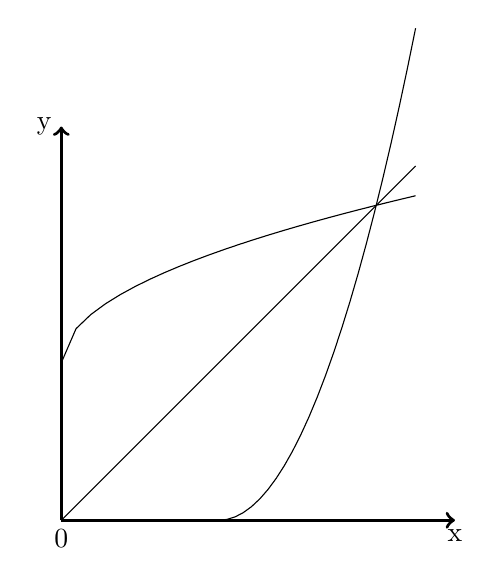
\begin{tikzpicture}[yscale=1, xscale=1]
\draw [->,very thick] (0,0) -- (0,5); \node [left] at (0,5) {y};
\draw [->,very thick] (0,0) -- (5,0); \node [below] at (5,0) {x};

\node [below] at (0,0) {0}; 

\draw [domain=0:4.5] plot (\x, {\x});
\draw [domain=0:4.5] plot (\x, {sqrt(\x) + 2});
\draw [domain=2:4.5] plot (\x, {(\x-2)*(\x-2)});
\end{tikzpicture} !$Db(f^{-1})$ ist nur $[2;\infty)$ obwohl $(x-2)^2$ für alle $x \in \mathbb{R}$ erklärt ist.

\subparagraph{Defnition 6} Die reellwertige Funktion $y=f(x)$ heißt
\begin{enumerate}
\item streng monoton wachsend, falls $x_1 < x_2 \Rightarrow f(x_1) < f(x_2)$
\item monoton wachsend (=nicht fallend), falls $x_1 < x_2 \Rightarrow f(x_1) \leq f(x_2)$
\end{enumerate}
für alle $x_1, x_2 \in Db(f)$ gilt.

Analog: streng monoton falled bzw. monoton fallend (=nicht wachsend)

\subparagraph{Satz 2} $f$ streng monoton $\Rightarrow f$ injektiv, (d.h. $f^{-1}$ existiert)

\subsubsection{Elementare Funktionen (Teil 2)}
\paragraph{Wurzel- und Logarithmusfunktionen}
\subparagraph{Definition 7}
\[ y = x^{\frac{1}{n}} = \sqrt[n]{x} \, (x\geq 0; n \in \mathbb{N}^*)\]
ist die Umkehrfunktion zu $y=x^n \, (x\geq 0, n \in \mathbb{N}^*)$\\
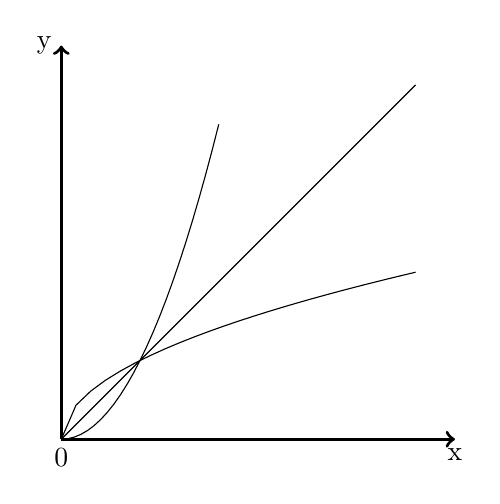
\begin{tikzpicture}[yscale=1, xscale=1]
\draw [->,very thick] (0,0) -- (0,5); \node [left] at (0,5) {y};
\draw [->,very thick] (0,0) -- (5,0); \node [below] at (5,0) {x};

\node [below] at (0,0) {0}; 

\draw [domain=0:2] plot (\x, {pow(\x,2)});
\draw [domain=0:4.5] plot (\x, {sqrt(\x)});
\draw [domain=0:4.5] plot (\x, {\x});
\end{tikzpicture}

Diskussion:
\begin{enumerate}
\item Im Bereich der reellen Zahlen ist $\sqrt[n]{x}$ nur für $x \geq 0$ erklärt, der Funktionswert selbst ist nicht negativ.
\item Lässt man in $x^{\frac{1}{n}}$ negative $x$ zu, (z.B. $ \sqrt[3]{-8} = -2$), so ergeben sich Widersprüche: $\sqrt[3]{-8}=-2 \Rightarrow -2 = (-8)^{\frac{1}{3}} = (-8)^{\frac{2}{6}}=((-8)^2)^{\frac{1}{6}} = 64^{\frac{1}{6}} = 2$\\* (die Lösungs der Gleichung $x^3 = -8$ ist natürlich $x=-2$)
\end{enumerate}

\subparagraph{Definition 8}
\[y=\log_a{x} \; (a>0, a\neq 1, x>0)\] ist die Umkehrfunktion zu $y=a^x \, (x\in \mathbb{R})$

speziell: $\lg{x}:= \log_{10}{x},\, \ln{x} := \log_e{x}$\\*
Achtung bei TR: (manchmal log=ln, auch log=lg)

Diskussion:
\begin{enumerate}
\item Log Gesetze (Basis beliebig):\\
$\log{xy} = \log{x} + \log{y}$\\
$\log{\frac{x}{y}}= \log{x} - \log{y}$\\
$\log{x^a} = a\log{x}$
\item Es gilt $a^x = e^{x \ln{a}} \; (= (\underbrace{e^{\ln{a}}}_{a})^x)$
\end{enumerate}

\paragraph{Arcusfunktionen}
Vorbetrachtung: $y=f(x) = \sin{x}$ ist nicht injektiv, also ex. keine Umkehrfunktion.\\
Aber $y=\sin{x}$ für $x\in [-2\frac{\pi}{2};\frac{\pi}{2} )$ ist injektiv, also umkehrbar.

\subparagraph{Definition 9} Umkehrfunktion der trigonometrischen Funktionen\\
\begin{tabular}{c|c|c||c}
 & Db & Wb & Umkehrfunktion von\\ \hline
$y=\arcsin{x}$ & $[-1;1]$ & $[-\frac{\pi}{2};\frac{\pi}{2}]$ & $y=\sin{x}, -\frac{\pi}{2} \leq x \leq \frac{\pi}{2}$\\ 
$y= \arccos{x}$ & $[-1;1]$ & $[0;\pi]$ & $y=\cos{x} , 0 \leq x \leq \pi$\\
$y = \arctan{x}$ & $\mathbb{R}$ & $(-\frac{\pi}{2} ; \frac{\pi}{2} )$ & $y= \tan{x}, -\frac{\pi}{2} < x < \frac{\pi}{2}$ \\
$y= \text{arccot} \,x$ & $\mathbb{R}$ & $(0;\pi)$ & $y=\cot{x}, 0<x<\pi$\\
\end{tabular}

Beispiel 5 Gesucht sind alle Lösungen der Gleichung $\tan{2x} = y$. Es sei $2x \in (-\frac{\pi}{2} + k \pi ; \frac{\pi}{2} + k\pi) \curvearrowright y=\tan{2x}=\tan{2x-k\pi} \text{ mit } 2x - k\pi \in (-\frac{\pi}{2} ; \frac{\pi}{2} )$\\
$\curvearrowright 2x - k\pi = \arctan{y} \curvearrowright \underline{\underline{ x = \frac{1}{2} (k\pi + \arctan{y}), k \in \mathbb{Z} }}$

\paragraph{Areafunktionen}
\subparagraph{Definition 10} Umkehrfunktionen der Hyperbelfunktionen\\*
\begin{tabular}{c|c|c|c}
area & Db & Wb & Umkehrfunktion von\\\hline
$y=\text{arsinh} \, x$ & $\mathbb{R}$ & $\mathbb{R}$ & $y=\text{sinh} \, x, x \in \mathbb{R}$\\
$y=\text{arcosh}\, x$ & $[1;\infty)$ & $[0;\infty)$ & $y=\text{cosh}\, x , x \geq 0$\\
$y=\text{arctanh}\, x$ & $(-1;1)$ & $\mathbb{R}$ & $y=\text{tanh}\, x , x \in \mathbb{R}$\\
$y=\text{arcoth}\, x$ & $ \mathbb{R} \backslash [-1;1]$ & $\mathbb{R} \backslash \{ 0 \} $ & $y=\text{coth}\, x, x\neq 0$\\

\end{tabular}\\
Aus der Definition 9 der Hyperbelfunktion folgt:\\*
\begin{tabular}{c|c}
$\text{arsinh}\, x = \ln{ (x + \sqrt{x^2+1})}$ & $ \text{artanh}\, x = \frac{1}{2} \ln{(\frac{1+x}{1-x} ) }$\\ \hline
$\text{arcosh}\, x = \ln{(x+\sqrt{x^2 -1})}$ & $\text{arcoth}\, x = \frac{1}{2} \ln{(\frac{x+1}{x-1})}$\\
\end{tabular}

\subsection{Lineare Algebra}
\subsubsection{Vektorräume}\label{VR}
Begriff:
\begin{enumerate}
\item \label{VR1} Gegeben seinen ein Körper $(K,+,\cdot)$, dessen Elemente Skalare heißen (meist $(\mathbb{R},+,\cdot)$ und eine \textsc{Abel}sche Gruppe $(V,\oplus)$ ($V$\dots Menge, Elemente heißen Vektoren, $\oplus$ \dots sogenannte Vektoraddition)
\item \label{VR2} Es gibt eine Abbildung $\odot$ von $K \times V \text{ in } V$, die jedem $x\in V$ und jedem $\lambda \in K$ ein Element $\lambda \odot x \in V$ zuordnet (die sogenannte Multiplikation eines Vektors mit einem Skalar) mit folgenden Eigenschaften:
\begin{itemize}
\item Distributivgesetze: $(\lambda + \mu ) \odot x = (\lambda \odot x) + (\mu \odot x)$\\
$\lambda \odot ( x \oplus y) = (\lambda \odot x ) \oplus (\lambda \oplus y)$
\item Assoziativgesetz: $(\lambda \cdot \mu) \odot x = \lambda \odot (\mu \odot x) $
\item $1\odot x = x$
\end{itemize}
\end{enumerate}
Eine Menge $V$ mit dem in (\ref{VR1}) und (\ref{VR2}) aufgeführten Operationen $\oplus$ und $\odot$ heißt Vektorraum (VR) über $K$.
Bemerkung Schreibweise meist  $\left\{ \begin{array}{rcl}
         +
         & \mbox{anstelle von}
         & \oplus \\ 
        \cdot
         & \mbox{anstelle von} 
         & \odot \\
                \end{array}\right.$

\subparagraph{Beispiel 1} Skalarbereich $K = \mathbb{R}$\\
Vektoren: Größen, die durch eine Zahlengröße (z.B. Länge) und eine Richtung charakterisiert sind (Z.B. Kräfte, Geschwindigkeiten, Translationen)

\begin{tikzpicture}
\draw [->,thick] (0,0) -- (3,3); \node [left] at (0,0) {P}; \node [above] at (1,1) {\underline{a}}; \node [right] at (3,3) {Q};

\draw [->,thick] (0,-2) -- (3,1); \node [left] at (0,-2) {R}; \node [above] at (1,-1) {\underline{a}}; \node [right] at (3,1) {S};
\end{tikzpicture} Pfeile als Repräsentation eines Vektors $\underline{a}$, Bezeichnung $\underline{a} = \overrightarrow{PQ} = \overrightarrow{RS}$ auch $\vec{a}$

Ortsvektoren: Angeheftet an einem gemeinsamen Anfangspunkt $0$ (Ursprung)

\begin{itemize}
\item Vektoraddition $\vec{a} + \vec{b}$
\item Multiplikation mit einem Skalar $\lambda \cdot \vec{a}$\\*
$\lambda > 0$ \dots gleiche Richtung\\*
$\lambda < 0$ \dots entgegengesetze Richtung\\
Länge: $\lvert \lambda \rvert \text{ -fache der Länge von }\vec{a}$
\item Subtraktion $\vec{a} - \vec{b} \;(:= \vec{a} + (-\vec{b}))$
\item Nullvektor $\vec{O}$ (Länge 0, keine Richtung)
\end{itemize}

\subparagraph{Beispiel 2} $K = \mathbb{R}, V=\{ 
\begin{pmatrix} x_1 \\ x_2 \\ \vdots \\ x_n \end{pmatrix} \vert x_1,x_2,\dots ,x_n \in \mathbb{R} \}$ (Menge der sogenannten Spaltenvektoren)
\begin{itemize}
\item Vektoraddition: $\begin{pmatrix} x_1\\ \vdots\\ x_n\end{pmatrix} + \begin{pmatrix} y_1\\ \vdots \\ y_n\end{pmatrix} := \begin{pmatrix} x_1 + y_1\\ \vdots \\ x_n + y_n\end{pmatrix}$
\item Multiplikation $\lambda \cdot \begin{pmatrix} x_1\\ \vdots\\ x_n\end{pmatrix} := \begin{pmatrix} \lambda \cdot x_1\\ \vdots\\ \lambda \cdot x_n\end{pmatrix}$
\end{itemize}

\subparagraph{Definition 1} Die Vektoren $\vec{a}_1, \dots \vec{a}_n$ heißen linear unabhängig, wenn die Gleichung \begin{equation} \label{VRDef1*} x_1 \vec{a}_1 + x_2 \vec{a}_2 + \dots + x_n \vec{a}_n = 0\end{equation}  nur die triviale Lösung $x_1=x_2=\dots = x_n=0$ besitzt.

Diskussion:
\begin{enumerate}
\item $x_1\vec{a}_1 + \dots + x_n\vec{a}_n$ heißt eine Linearkombination (LK) der Vektoren $\vec{a}_1,\dots , \vec{a}_n$
\item Falls es eine LK der Gestalt (\ref{VRDef1*} ) gibt, in der nicht alle $x_i$ gleich 0 sind, so heißen $\vec{a}_1,\dots , \vec{a}_n$ linear abhängig.\\
In diesem Falle lässt sich (wenigstens) einer der Vektoren als LK der anderen darstellen.
\end{enumerate}
\subparagraph{Definition 2} Es sei $V_1 \subseteq V$ eine nichtleere Teilmenge von $V$. Wir bezeichnen mit $L(V_1)$ die Menge aller LK von jeweils endlich vielen Vektoren aus $V_1$.\\
$L(V_1)$ heißt lineare Hülle von $V_1$

Bemerkung: $L(V_1)$ ist selbst ein VR, der von $V_1$ aufgespannte Teilraum von $V$.

\subparagraph{Definition 3}
\begin{itemize}
\item Ein VR $V$ heißt $n$-dimensional, wenn es $n$ unabhängige Vektoren $\vec{a}_1, \dots , \vec{a}_n$ gibt, die den gesamten Raum aufspannen: $V=L(\vec{a}_1, \dots ,\vec{a}_n)$
\item Die Menge der Vektoren $\vec{a}_1 , \dots ,\vec{a}_n$ nennt man in diesem Falle eine Basis von $V$.
\end{itemize}

Diskussion: In jedem VR gibt es unterschiedliche Basen, jedoch ist die Anzahl der Vektoren, die eine Basis bilden stets gleich (Dimension von VR).

\subparagraph{Satz 1} Es sei $\vec{a}_1, \dots , \vec{a}_n$ eine Basis eines VR $V$. Dann gibt es für jedes $x \in V$ eine eindeutige Darstellung der Gestalt $x=x_1\vec{a}_1 + x_2\vec{a}_2 + \dots + x_n \vec{a}_n$.

Bemerkung: Die Koeffizienten $x_1, \dots , x_n$ heißen Koordinaten von $\vec{x}$ bezüglich der Basis $\vec{a}_1, \dots , \vec{a}_n$.\\
Die Summanden $x_1 \vec{a}_1, \dots , x_n \vec{a}_n$ heißen Komponenten von $\vec{x}$ bezüglich der Basis $\vec{a}_1, \dots , \vec{a}_n$.

\subparagraph{Bespiel 3} (vlg. Beispiel 2)
Nullvektor im Raum der Spaltenvektoren: $\vec{a} = \begin{pmatrix}
0\\
0\\
\vdots\\
0
\end{pmatrix}$\\
Der Raum selbst heißt $\mathbb{R}^n$\\
Die Vektoren $\vec{e}_1 = \begin{pmatrix} 1\\0\\ \vdots \\ 0\end{pmatrix}, \vec{e}_2 = \begin{pmatrix} 0\\1\\ \vdots \\ 0\end{pmatrix}, \dots , \vec{e}_n \begin{pmatrix} 0\\0\\ \vdots \\ 1\end{pmatrix}$ des Raumes $\mathbb{R}^n$ bilden offensichtlich eine Basis von $\mathbb{R}^n$
\subparagraph{Beispiel 4} Zwei Vektoren $\vec{a}_1 \neq 0 $ und $\vec{a}_2 \neq 0$ in einer Ebene bilden genau dann eine Basis, wenn sie nicht parallel sind.

\subsubsection{Matrizen}
\subparagraph{Definition 4} Ein aus $m\cdot n $ Zahlen $a_{ij} \in \mathbb{R}$, welche in $m$ Zeilen und $n$ Spalten angeordnet sind, bestehendes Schema heißt Matrix vom Typ $(m,n)$.

$\underline{A}=
\begin{pmatrix}
a_{11} & a_{12} & \dots & a_{1n}\\
a_{21} & a_{22} & \dots & a_{2n}\\
\vdots & \vdots & \ddots & \vdots\\
a_{m1} & a_{m2} & \dots & a_{mn}\\
\end{pmatrix}
=(a_{i j}), \; \underbrace{i}_{Zeilenindex}=1,...,m \underbrace{j}_{Spaltenindex}=1,...,n$

\subparagraph{Rechenoperationen}
\subparagraph{Definition 5} $\underline{A} = (a_{ij}), \, \underline{B}=(b_{ij})$ seinen vom gleichen Typ $(m,n)$.
\begin{enumerate}
\item \label{MaRe1} $\underline{A} + \underline{B} := ( a_{ij} + b_{ij})\quad  i=1,...,m  \; j=1,...,n \text{ \dots Matr.-Addition}$
\item\label{MaRe2} $\text{Es sei } \lambda \in \mathbb{R},\, \underline{A} = (a_{ij}) \quad  i=1,...,m  \; j=1,...,n$\\*
$\lambda \cdot \underline{A} := (\lambda a_{ij}) \quad  i=1,...,m  \; j=1,...,n$
\item \label{MaRe3} $\underline{A} = (a_{ij})$ sei vom Typ $(m,n)$\\
$\underline{B} = (b_{jk})$ sei vom Typ $(n,p)$\\
$\underline{A}$ und $\underline{B}$ heißen in dieser Reihenfolge verkettet. (Spaltenzahl von $\underline{A} =$ Zeilenzahl von $\underline{B}$). Dann:\\
$\underline{A} \cdot \underline{B} = ( \sum\limits_{j=1}^n a_{ij} b_{jk} )\quad i=1,...,m \, k=1,...,p$ (Matr.-Multiplikation)\\*
Das Produkt ist also vom Typ $(m,p)$
\end{enumerate}

Diskussion: Zweckmäßig \textsc{Falk}-Schema für die Matr.-Multiplikation (vgl. Beispiel 5).

\subparagraph{Definition 6} Die aus der $(m,n)$-Matrix $\underline{A}$ durch Vertauschen von Zeilen und Spalten entstehende $(n,m)$-Matrix heißt die Transponierte von $\underline{A}$.\\*
Bezeichnung $\underline{A}^T$

Beispiel 5: $\underline{A}= \begin{pmatrix}
5&-3\\
1&4
\end{pmatrix}, \underline{B}= \begin{pmatrix}
3&6&4\\
-2&0&1
\end{pmatrix}, \underline{C} = \begin{pmatrix}
-1&5\\
0&3
\end{pmatrix}$
\begin{enumerate}
\item $\underline{A} + \underline{B}$ existiert nicht (unterschiedlicher Typ)
\item $\underline{A} + \underline{C} = \begin{pmatrix}
4&2\\
1&7 \end{pmatrix}$
\item $2 \cdot \underline{A} = \begin{pmatrix}10&-6\\ 2 & 8 \end{pmatrix}$
\item $\underline{B}^T= \begin{pmatrix}
3&-2\\
6&0\\
4&1 \end{pmatrix}$
\item $\underbrace{\underbrace{\underline{B}}_{(2,3)} \cdot \underbrace{\underline{A}}_{(2,2)}}_{3 \neq 2 \curvearrowright \text{ nicht verkettet}}$ existiert nicht
\item $\underline{A} \cdot \underline{B}$ \textsc{Falk}-Schema
%Todo 2013-12-11T11:47
\end{enumerate}

Bemerkung: Matrizen-Multiplikation ist im allgemeinen nicht kommutativ!

Diskussion (Ausgewählte Rechenregeln)
\begin{enumerate}
\item Die Menge der Matrizen vom gleichen Typ bildet mit den Operationen (\ref{MaRe1}) und (\ref{MaRe2}) aus Definition 5 einen VR (Vektorraum).
\item Falls die entsprechenden Typ-Vorraussetzungen erfüllt sind, gelten:
\begin{itemize}
\item $(\underline{A} \underline{B} ) \underline{C} = \underline{A} (\underline{B} \underline{C})$ (Assoziativgesetz)
\item $\underline{A} (\underline{B} + \underline{C}) = \underline{A} \underline{B} + \underline{A} \underline{C}$\\
$(\underline{A} + \underline{B}) \underline{C} = \underline{A} \underline{C} + \underline{B} \underline{C}$ (Distributivgesetze)
\item $(\lambda \underline{A})^T = \lambda \cdot \underline{A}^T,\, (\underline{A}^T)^T = \underline{A}$
\item $(\underline{A} + \underline{B})^T = \underline{A}^T + \underline{B}^T, \, (\underline{A} \underline{B})^T = \underline{B}^T \underline{A}^T$ 
\end{itemize}
\item Achtung: Im allg. gilt $\underline{A} \underline{B} \neq \underline{B} \underline{A}$
\item \textsc{Falk}-Schema bei fortgesetzer Multiplikation $\underline{A} \underline{B} \underline{C}$:\\
\begin{tabular}{c|c|c}
 & $\underline{B}$ & $\underline{C}$\\ \hline
$\underline{A}$ & $\underline{A} \underline{B}$ & $(\underline{A} \underline{B}) \underline{C}$
\end{tabular} oder
\begin{tabular}{c|c}
 & $\underline{C}$\\ \hline
$\underline{B}$ & $\underline{B} \underline{C}$\\ \hline
$\underline{A}$ & $\underline{A} (\underline{B} \underline{C})$
\end{tabular}
\end{enumerate}

Spezielle Matrizen:
\begin{enumerate}
\item Quadratische Matrizen: Typ $(n,n)$\\
Eine quadratische Matrix $\underline{A}$ heißt
\begin{enumerate}
\item symmetrisch, wenn $\underline{A}^T = \underline{A}$ gilt
\item obere/untere Dreiecksmatrix, wenn $a_{ij} = 0$ für $\left\{ \begin{array}{lr}
         i > j
         &   \\%Todo 2013-12-11T12:08 
         i < j
         &  \\
                \end{array}\right.$
\item Diagonalmatrix, wenn $a_{ij}=0$ für $i/neq j$
\item Einheitsmatrix $underline{E}$, wenn $a_{ij}= \left\{ \begin{array}{rcl}
         1
         & \mbox{für}
         & i = j \\ 
        0
         & \mbox{für} 
         & i \neq j \\
                \end{array}\right.$\\
(spezielle Diagonalmatrix, oft auch mit $\underline{I}$ bezeichnet)
\end{enumerate}
\item Nullmatrix $\underline{0}$ (saämtliche Elemente $=0$; nicht notwendig quadratisch)
\item Matrizen vom Typ $(n,1)$ ($n$ Zeilen, 1 Spalte) heißen (Spalten-)Vektoren\\
$\underline{a}= \begin{pmatrix} a_1\\a_2\\ \vdots \\ a_n \end{pmatrix} \in \mathbb{R}^n$, vgl. \ref{VR}\\
Es ist dann $\underline{a}^T = (a_1 | a_2 | ... | a_n)$ vom Typ $(1,n)$ (Zeilenvektor)
\end{enumerate}

Diskussion:
\begin{enumerate}
\item Die quadratischen Matrizen vom Typ $(n,n)$ bilden mit den Operationen Matr-Add. und Matr.-Multipl. einen nicht-kommutativen Ring.
\item Für quadratische Matrizen $/underline{A}$ sind Potenzen bildbar:
\[ \underline{A}^0 := \underline{E},\, \underline{A}^n = \underbrace{\underline{A} \cdot \underline{A} \cdot ... \cdot \underline{A}}_{n \text{ Faktoren}}, \; n \in \mathbb{N}^*\]
\item Falls die entsprechenden Typ-Vorraussetzungen erfüllst sind, gelten:\\
\begin{tabular}{c|c|c}
$\underline{A} \cdot \underline{E} = \underline{A}$ & $\underline{0} \cdot \underline{A} = \underline{0}$ & $\underline{A} + \underline{0} = \underline{A}$\\
$\underline{E} \cdot \underline{A} = \underline{A}$ & $ \underline{A} \cdot \underline{0} = \underline{0}$ & \\
\end{tabular}\\*
(analog 0 bzw. 1 bei reelllen Zahlen)
\item Es sei $\underline{A}$ vom Typ $(m,n),\, \underline{x} \in \mathbb{R}^n,$ d.h. vom Typ $(n,1)$\\
Dann ist $\underline{y}=\underbrace{\underline{A}}_{(m,n)}\, \underbrace{\underline{x}}_{(n,1)}$ vom Typ $(m,1)$, also $\underline{y} \in \mathbb{R}^m$\\
Durch die Zuordnung $\underline{x} \mapsto \underline{A} \, \underline{x}$ wird eine lineare Abbildung von $\mathbb{R}^n \text{ in } \mathbb{R}^m$ beschrieben. (Eine Abb. $f$ heißt linear, wenn $f(x+y) = f(x) + f(y), \, f(a\cdot x) = a \cdot f(x) \; (\forall x,y \in Db(f), \forall a \in \mathbb{R})$ gilt.)
\end{enumerate}

$\underline{y}=\underbrace{\underline{A}}_{(m,n)}\, \underbrace{\underline{x}}_{(n,1)}$ ausführlich mit \textsc{Falk}-Schema: %Todo 2013-12-11T12:33

d.h. $\begin{pmatrix}
a_{11} x_1 + \dots + a_{1n} x_n = y_1\\
\vdots \\
a_{m1} x_1 + \dots + a_{mn} x_n = y_m
\end{pmatrix} \Leftrightarrow \underline{A}\, \underline{x} = \underline{y} \implies$ Matrix-Schreibweise für ein lineares Gleichungssystem

\subsubsection{Determinanten}
\subparagraph{Definition 7} Jeder $n$-reihigen quadratischen Matrix $\underline{A}$ ist eindeutig eine Zahl $\det{\underline{A}}$, die sogenannte Determinante von $/underline{A}$, wie folgt zugeordnet:\\
$n=1 : \det(a_{11} := a_{11}$\\*
$n\geq 2: \det{ \begin{pmatrix}
a_{11} & \dots & a_{1n}\\
\vdots & \ddots & \vdots\\
a_{n1} & \dots & a_{nn} \end{pmatrix}} := a_{11} A_{11} + a_{12} A_{12} + ... + a_{1n}A_{1n}$\\
Dabei ist $A_{ij} = (-1)^{i+j} \det{\underline{U}_{ij}}$ die Adjunkte des Elements $a_{ij}$

$\underline{U}_{ij} \dots (n-1)$-reihige (Unter-)Matrix, die durch Streichen der $i$-ten Zeile und der $j$-ten Spalte von $\underline{A}$ entsteht.\\
Bezeichnung: $\det{\underline{A}} = \det{()} \underbrace{=}_{n\geq 2} \begin{vmatrix} a_{11} & \dots & a_{1n} \\ \vdots & & \vdots \\ a_{n1} & \dots & a_{nn} \\ \end{vmatrix}$

\subparagraph{Satz 2}
\begin{enumerate}
\item $\det{(\underline{A}\cdot \underline{B})} = \det{\underline{A}} \cdot \det{\underline{B}}$
\item \label{2b} $\det{(\underline{A}^T)} = \det{\underline{A}}$
\end{enumerate}
Wegen Satz 2 \ref{2b} gelten alle im folgenden für die Zeilen formulierten Eigenschaften sinngemäß auch für die Spalten.

\subparagraph{Satz 3} Eigenschaften der Determinanten
\begin{enumerate}
\item $\underline{B}$ gehe aus $\underline{A}$ durch Vertauschen zweier Zahlen hervor. Dann gilt $\det{\underline{B}} = - \det{\underline{A}}$
\item Es gilt $\det{\underline{A}} = 0$, falls zwei Zeilen elementweise proportional sind, bzw. falls alle Elemente einer Zeile gleich $0$ sind.
\item Es gilt:
$\rightarrow \begin{vmatrix}
a_{11} & \dots & a_{1n}\\
\vdots &  & \vdots\\
\lambda \cdot a_{i1} & \dots & \lambda \cdot a_{in}\\
\vdots & & \vdots\\
a_{n1} & \dots & a_{nn}\\
\end{vmatrix} =  \lambda \cdot \begin{vmatrix}
a_{11} & \dots & a_{1n}\\
\vdots & & \vdots\\
a_{i1} &\dots & a_{in}\\
\vdots & & \vdots\\
a_{n1} & \dots & a_{nn}\\
\end{vmatrix}$
\item \label{E4}Der Wert einer Determinante ändert sich nicht, wenn das $\lambda$-fache einer Zeile elementweise zu einer anderen Zeile addiert wird.
\item \label{E5} $\det{\underline{A}} = \sum\limits_{j=1}^{n} a_{ij} A_{ij}$ (Entwicklung nach $i$-ter Zeile, $i=1,...,n$)\\*
$\det{\underline{A}} = \sum\limits_{i=1}^{n} a_{ij} A_{ij}$ (Entwicklung nach $j$-ter Spalte, $j=1,...,n$)\\*
(Entwicklungssatz)
\end{enumerate}

\subparagraph{Beispiel 7} Prinzip: Nullen erzeugen mit (\ref{E4}), Entwicklungssatz  (\ref{E5}) anwenden.

\subparagraph{Anwendungen}
\begin{enumerate}
\item Vektorrechnung in $\mathbb{R}^3$, vgl. Abschnitt 1.5.5.
\item Gegebenes lineares Gleichungssystem ($n$ Gleichungen, $n$ Unbekannte)\\
Matrix-Form $\underline{A}\, \underline{x} = \underline{b}$ mit $\underline{A} = (a_{ij}), \, \underline{x} = \begin{pmatrix} x_1 \\ \vdots \\ x_n\\ \end{pmatrix}, \underline{b}= \begin{pmatrix} b_1 \\ \vdots \\ b_n\\ \end{pmatrix}$\\
$\underline{A}\, \underline{x} = \underline{b}$ besitzt genau dann eine Lösung eindeutige Lösung $\underline{x}$, wenn $\det{\underline{A}} \neq 0$.\\
In diesem Falle gilt $x_j = \frac{\det{\underline{B_j}}}{\det{\underline{A}}} \; (j=1, ... ,n)$, wobei $\underline{B}_j$ aus $\underline{A}$ hervorgeht, indem die $j$-Spalte von $\underline{A}$ durch $\underline{b}$ ersetzt wird. (\textsc{Cramer}sche Regel, theoretische Bedeutung, praktisches Vorgehen vgl. folgenden Abschnitt 1.5.4)

\end{enumerate}

\subsubsection{Lineare Gleichungssysteme, Rang einer Matrix, Inverse}
\paragraph{Das Austauschverfahren}
Gegeben: System von $m$ linearen Funktionen mit den unabhängigen Variablen $x_1,...,x_n$ und den abhängigen Variablen $y_1,...,y_m$:\\
$y_1 = a_{11} x_1 + \dots + a_{1n} x_n + a_{10}\\
\vdots\\
y_m = a_{m1} x_1 + \dots + a_{mn} x_n + a_{m0}$

\subparagraph{Beispiel 8} Betrieb, $m$ Abteilungen, $n$ Produkte $P_1,...,P_n$\\
$a_{ij}$ \dots Kosten pro Einheit von $P_j$ die in Abteilung $i$ entstehen\\
$a_{i0}$ \dots Fixkosten in Abteilung $i$\\
$x_j$ \dots produzierte Menge von $P_j$\\
$y_i$ \dots Gesamtkosten in Abteilung $i$\\

Matrix Schreibweise $\underline{y} = \underline{A} \, \underline{x} + \underline{a}$ mit $\underline{A}=(a_{ij}), \, \underline{a} = \begin{pmatrix} a_{10}\\ \vdots \\ a_{m0}\\ \end{pmatrix} \in \mathbb{R}^m$

Tabellenform: \begin{tabular}{c|cccc}
 & $x_1$ & \dots & $x_n$ & 1\\ \hline
$y_1$ & $a_{11}$ & \dots & $a_{1n}$ & $a_{10}$\\
\vdots & \vdots & & \vdots & \vdots \\
$y_m$ & $a_{m1}$ & \dots & $ a_{mn}$ & $a_{m0}$\\
\end{tabular} kurz
\begin{tabular}{c|cc}
 & $\underline{x^T}$ & 1\\ \hline
$\underline{y}$ & $\underline{A}$ & $\underline{a}$\\
\end{tabular} (T1)

Aufgaben:\begin{enumerate}
\item $\underline{x}$ vorgegeben, $\underline{y}$ ist zu berechnen (klar)
\item $\underline{y}$ vorgegeben, $\underline{x}$ ist zu berechnen (nicht immer lösbar, falls lösbar, nicht immer eindeutig lösbar)
\end{enumerate}

Lösungsprinzip: Man tausche so oft wie möglich $y_r$ gegen $x_s$ aus = Austauschschritt AS $(y_r \leftrightarrow x_s)$ Austauschverfahren

AS $y_r \leftrightarrow x_s$ bedeutet
\begin{enumerate}
\item $r$-te Zeile $y_r = \dots$ auflösen nach $x_s \curvearrowright x_s= \dots$
\item in allen anderen Zeilen $x_s$ durch die rechte Seite von $x_s \curvearrowright x_s= \dots$ ersetzen $\curvearrowright$ neue Tabelle T2
\end{enumerate}
Die Koeffizienten $a_{ij}^*$ in der neuen Tabelle, entstehen aus den alten Koeffizienten $a_{ij}$ wie folgt:

Austauschregeln\\
Abkürzungen: $p:= a_{rs}$ (Pivot)\\*
PZ \dots Pivotzeile (Zeile r)\\*
PS \dots Pivotstpalte (Spalte s)
\begin{enumerate}
\item \label{AR1} $a_{rs}^* = \frac{1}{p}$
\item \label{AR2} $a_{rj}^* = \frac{a_{rj}}{(-p)} \; (j \neq s)$\\
"`neue PZ = alte PZ / (-Pivot)"'
\item \label{AR3} $a_{is}^* = \frac{a_{is}}{p}\; (i \neq r)$ d.h.\\
"`neue PS = alte PS /Pivot"'
\item \label{AR4} $a_{ij}^* = a_{ij} + a_{is} \cdot a_{rj}^* \; (i \neq r, j \neq s)$
\end{enumerate}

Praktisches Vorgehen
\begin{enumerate}
\item Pivot kennzeichnen
\item Austauschregeln AR1 - AR4 abarbeiten.\\
Dabei für AR3 unter alter Tabelle die neue PZ als Kellerzeile schreiben.
\end{enumerate}

$\begin{pmatrix}
 & & \text{Spalte } j & \dots & \text{Spalte } s & \\
 & & \vdots & & \vdots \\
\text{Zeile } i & \dots & a_{ij} & \dots & a_{is} & \dots \\
\vdots & & \vdots & &\vdots \\
\text{Kellerzeile } K & \dots & a_{rj}^* & \dots & * & \dots \\
\end{pmatrix}$\\
$a_{ij}^* = a_{ij} + a_{is} \cdot a_{rj}^*$

\subparagraph{Varianten des Austauschverfahrens (AV)}
\begin{enumerate}
\item AVZ \dots AV mit Zeilentilgung, d.h. neue PZ in neuer Tabelle weglassen
\item AVS \dots AV mit Spaltentilgung,d.h. in neuer Tabelle neue PS weglassen\\
(nur anwendbar, wenn Variable über der wegzulassenden Spalte $=0$ ist, vgl. 1.5.4 Lineare Gleichungssysteme )
\item AVSZ \dots AVS + AVZ gleichzeitig
\end{enumerate}

\paragraph{Lineare Gleichungssysteme}
\begin{itemize}
\item Gegeben sei das lineare Gleichungssystem (in Gleichungen mit $n$ Unbekannten $x_1,...,x_n)$\\
\begin{equation} \label{GS1} \begin{array}{c} a_{11} x_1 + \dots + a_{1n} x_n = b_1\\
\vdots \\
a_{m1} x_1 + \dots + a_{mn} x_n = b_m \end{array} \end{equation}
\item Gleichungssystem (\ref{GS1}) heißt homogen, falls $b_1 = b_2 = ... = b_m = 0$, sonst inhomogen
\item Matrixform $\underline{A} \, \underline{x} = \underline{b} \Leftrightarrow \underline{A} \, \underline{x} - \underline{b} = 0$
\item Äquivalente Form: \begin{equation} \label{GS1'} \begin{array}{c} \underline{y} = \underline{A} \, \underline{x} - \underline{b} \text{ mit } \underline{y} = \begin{pmatrix} y_1 \\ \vdots \\ y_m \end{pmatrix} = \underline{0} \\ \text{Hilfsgrößen } y_1= ... = y_m = 0  \end{array} \end{equation}
\item Tabellenform:
\begin{tabular}{c|cc}
 & $\underline{x}^T$ & 1 \\ \hline
$\underline{y}$ & $\underline{A}$ & $-\underline{b}$
\end{tabular}
\item Lösungsprinzip: AVS
\begin{itemize}
\item Fall 1: Alle $y$, sind austauschbar $\Rightarrow $ (\ref{GS1}) ist lösbar, Lösung ist aus letzter Tabelle (TE) ablesbar.
\begin{tabular}{c|cc}
TE & $x_3$ & 1\\ \hline
$x_1$ & 0 & 4 \\
$x_2$ & 2 & -3 \\
\end{tabular} $x_1 = 4 \; x_2 = 2 x_3 -3 (x_3 \in \mathbb{R},$ frei wählbar)
\item Fall 2: Wenigstens ein $y_i$ ist gegen kein $x_j$ austauschbar\\
$\begin{array}{c|ccccc}
 & \text{eventuell noch nicht ausgetauschte } x_j & & & & 1\\ \hline 
\vdots \\
y_i & 0 & \dots & 0 & 0 & \alpha \\
\vdots \\
\end{array}$
$\curvearrowright y_i = \alpha $
\item Fall 2a: $\alpha = 0$ Zeile $y$, kann gestrichen werden ($0=0$)
\item Fall 2b $\alpha \neq 0 \curvearrowright$ Gleichungssystem (\ref{GS1} ) nicht lösbar (Widerspruch da $y_i = 0$ )
\end{itemize}
Diskussion: Verfahren endet also entweder im Fall 2b (unlösbar) oder in Tabelle in der kein $y_i$ mehr vorkommt (Fall 1 bzw. 2a):\\
$\begin{array}{c|ccccc} 
TE & x_{s1} & x_{s2} & \dots & x_{sq} & 1 \\ \hline
x_{r1} \\
\vdots \\
x_{rp} 
\end{array}$ (Darstellung 2)

\item $x_{r1}, ..., x_{rp}$ (ausgetausche $x_j$) \dots Basisvariable (BV)\\
$x_{s1}, ... , x_{sq}$ (nicht ausgetauschte $x_j$) \dots Nichtbasisvariable (NBV)\\
$(p + q = n )$
\item Allgemeine Lösung ergibt sich aus Endtabelle:\\
NBV frei wählbar (Parameter $\in \mathbb{R}$\\*
BV daraus berechenbar
\item Falls keine NBV vorhanden $\curvearrowright$ Lösung eindeutig
\end{itemize}
\subparagraph{Definition 8} Die Darstellung (2) heißt Basisdarstellung des lineare Gleichungssystems (\ref{GS1})

Diskussion: Aus einer Basisdarstellung (2) lassen sich weitere gewinnen durch Austausch $\underbrace{x_{ri}}_{BV} \leftrightarrow \underbrace{x_{sj}}_{NBV}$

\subparagraph{Beispiel 9}
$3 x_1 + x_2 + 2x_3 = -2$\\
$-5x_1 -3x_2 -2x_3 = -2 $ \\
$x_1 + 3x_2 -2 x_3 = 10 $\\
$\begin{array}{c|cccc}
T1 & x_1 & x_2 & x_3 & 1 \\ \hline
y_1 = 0 & 3 & 1 & 2 & 2 \\
y_2=0 & -5 & -3 & -2 & 2\\
y_3 = 0 & 1 &3 & -2 & -10 \\ \hline
K & -3 & * & -2 & -2 
\end{array}$\\
$\begin{array}{c|ccc}
T2 & x_1 & x_3 & 1\\ \hline
x_2 & -3 & -2 & -2 \\
0 & 4 & 4 & 8 \\
0 & -8 & -8 & -16 \\ \hline
K & * & -1 & -2
\end{array}$\\
$\begin{array}{c|cc}
T3 & x_3 & 1 \\ \hline
x_2 & 1 & 4 \\
x_1 & -1 & -2 \\
0 & 0 & 0 \\ \hline
\end{array}$ (Fall 2a: $0=0$ )

T3 ist Endtabelle (BV $x_1, x_2,$ NBV: $x_3$)\\
allg. Lösung: $x_2 = x_3 +4 \, x_1 = -x_3 -2 \, x_3 \in \mathbb{R}$ (frei wählbar)\\
andere Form mit Parameter $x_3 = t$: \\
$\underline{x} = \begin{pmatrix} -t -2 \\ t+4 \\ t \end{pmatrix}, t \in \mathbb{R}$

Bemerkungen:
\begin{enumerate}
\item Bei homogenen Systemen $\underline{A} \, \underline{x} = \underline{0}$ muss die 1-Spalte nicht geschrieben werden, nur "`gedacht"'
\item Die Methode AVS entspricht dem sogenannten \textsc{Gauss-Jordan}-Verfahren
\end{enumerate}

\subparagraph{Der Gausssche Algorithmus} (siehe Beispiel 10)
\begin{itemize}
\item AVSZ (Spalten und Zeilentilgung)
\item weggelassen Zeilen merken (Kellerzeilen)
\item Rückrechnung
\end{itemize}
\subparagraph{Beispiel 10}
$-x_1 + 2x_2 + 2x_3 = 4$\\
$2 x_1 + 5x_2 + 2x_3 = 4$\\
$2x_1 + x_2 -4 x_3 = -3$\\

$
\begin{array}{cc}
\begin{array}{c|cccc}
T_1 & x_1 & x_2 & x_3 & 1\\ \hline
0 & -1 & 2 & 2 & -4 \\
0 & 2 & 5 & 2 & -4\\
0 & 2 & 1 & -4 & 3 \\ \hline
x_2 & -2 & * & 4 & -3\\
\end{array}
&
\begin{array}{c|ccc}
T_2 & x_1 & x_3 & 1\\ \hline
0 & -5 & 10 & -10 \\
0 & -8 & 22 & -19\\ \hline
x_1 & * & 2 & -2\\ 
\end{array} \\
\begin{array}{c|cc}
T_3 & x_3 & 1\\ \hline
0 & 6 & -3 \\ \hline
x_3 & * & \frac{1}{2} \\ 
\end{array} & \text{\textsc{Ende AVSZ}}\\
\end{array}$\\
Rückrechnung: $T3 \curvearrowright x_3 = \frac{1}{2}$\\
$T2 \curvearrowright x_1 = 2x_3 -2 = \underline{\underline{-1}}$\\
$T1 \curvearrowright x_2 = -2x_1 + 4x_3 -3 = \underline{\underline{1}}$\\
Lösung: $\underline{\underline{\underline{x} = (-1 | 1 | \frac{1}{2} )^T}}$\\
Bemerkung: $m$ Gleichungen, $n$ Unbekannte\\
$m<n \curvearrowright$ \textsc{AVS} günstiger\\
$m \geq n \curvearrowright$ \textsc{Gauss} oder \textsc{AVS}

\paragraph{Weitere Anwendungen des AV}
\begin{enumerate}
\item Lineare Unabhängigkeit von Vektoren $\underline{a}_1, ... , \underline{a}_n \in \mathbb{R}^m$ überprüfen.\\
Ansatz: $x_1a_1 + x_2 a_2 + ... + x_n\underline{a_n} = \underline{0} \leftrightarrow \underline{A} \underline{x} = \underline{0}$ \\
mit $\underline{A} = (\underline{a}_1 | \underline{a}_2 | ... | \underline{a}_n)$\\
(homogens System, \textsc{AVS} mit Starttabelle $\begin{array}{c|c} & \underline{x}^T \\ \hline \underline{0} & \underline{A}\\ \end{array} $)
\begin{itemize}
\item Unabhängigkeit genau dann, wenn alle $x_i$ ausgetauscht werden können
\item Die zu den ausgetauschten $x_i$ (d.h. den Basisvariablen \textsc{AV}) gehörenden $\underline{a}_i$ sind unabhängig. Sie bilden eine Basis zu $L(\underline{a}_1,...,\underline{a}_n)$
\end{itemize}
\item Rang einer Matrix $\underline{A}= (a_1 | a_2 | ... | a_n) ... \text{rang}\, (\underline{A})$\\
Definition $\text{rang} \, (\underline{A}) = \dim{L (a_1, ... ,a_n)}$\\
Dimension des von den Spaltenvektoren aufgespannten Teilraumes (von $\mathbb{R}^m $)\\
Berechnung: $\text{rang}\, (\underline{A}) =$ Anzahl der ausführbaren Austauschschritte in \textsc{AVSZ} mit Starttabelle $\begin{array}{c|c} & \underline{x}^T\\ \hline \underline{y} & \underline{A} \end{array}$
\item Berechnung der Determinante einer $(n,n)$ -Matrix\\
vgl. Merkblatt LAG
\end{enumerate}

\paragraph{Die Inverse einer $(n,n)$ -Matrix}
\subparagraph{Definition 9} Es sei $\underline{A}$ vom Typ $(n,n)$. Das Gleichungssystem $\underline{y} = \underline{A}\, \underline{x}$ sei für jedes $\underline{y}$ eindeutig nach $\underline{x}$ auflösbar, d.h. $\underline{x} = \underline{B} \, \underline{y}$. Dann heißt die $(n,n)$-Matrix $\underline{B}$ Inverse zu $\underline{A}$.\\
Bezeichnung: $\underline{A}^{-1} := \underline{B}$\\
Falls $\underline{A}^{-1}$ existiert, so heißt $\underline{A}$ regulär, sonst singulär.

Bemerkungen:
\begin{enumerate}
\item $\underline{A}$ ist regulär $\leftrightarrow \det{\underline{A}} \neq 0 $
\item $\underline{A}$ regulär, dann hat $\underline{A} \, \underline{x} = \underline{b}$ die Lösung $\underline{x} = \underline{A}^{-1} \underline{b}$
\end{enumerate}

Rechenregeln: $A$ und $B$ seien regulär. Dann gelten $A A^{-1} = E,  A^{-1} A = E, (A^{-1})^{-1} = A$\\
$(AB)^{-1} = B^{-1} A^{-1}, \quad (A^T)^{-1} = (A^{-1})^T$

Bemerkung: Die Menge der regulären Matrizen vom Typ $(n,n)$ beildet mit der Operation "`Matrizen-Multiplikation"' eine (nicht \textsc{Abel}sche) Gruppe mit neutralem Element $\underline{E}$.

Verfahren zur Ermittlung der Inversen
\begin{itemize}
\item vollständiges \textsc{AV} mit Starttabelle $\begin{array}{c|c} T_1 & \underline{x}^T \\ \hline \underline{y} & \underline{A} \end{array}$\\
Fall 1: alle $x_j$ sind austauschbar $\curvearrowright \underline{A}$ regulär\footnote{nach Ordnen von Zeilen und Spalten ist $\underline{A}^{-1}$ aus TE ablesbar}
\item Probemöglichkeit $\underline{A}\, \underline{A}^{-1} = \underline{E}$
\end{itemize}

Beispiel 11:
%$\underline{A} = \begin{pmatrix} 1&2&1 \\ 1 &0 & 2\\ 1&-1&1 \end{pmatrix} \text{ ,gesucht } \underline{A}^{-1}.$\\
%$\begin{array}{ccc}
%\begin{array{c|ccc}
%T_1 &x_1 &x_2 & x_3\\ \hline
%y_1 & 1 & 2 & 1\\
%y_2 & 1 & 0 & 2\\
%y_3 & 1 & -1 & 1\\ \hline
%K & * &-2 &-1
%\end{array}
%&
%\begin{array{c|ccc}
%T_2 &y_1 &x_2 & x_3\\ \hline
%x_1 & 1 & -2 & -1\\
%y_2 & 1 & -2 & 1\\
%y_3 & 1 & -3 & 0\\ \hline
%K & -1 &2 &*
%\end{array}
%&
%\begin{array{c|ccc}
%T_3 &y_1 &x_2 & y_2\\ \hline
%x_1 & 2 & -4 & -1\\
%x_3 & -1 & 2 & 1\\
%y_3 & 1 & -3 & 0\\ \hline
%K & \frac{1}{3} &* &0
%\end{array}\\
%\begin{array{c|ccc}
%T_4 &y_1 &y_3 & y_2\\ \hline
%x_1 & \frac{2}{3} & \frac{4}{3} & -1\\
%x_3 & -\frac{1}{3} & -\frac{2}{3} & 1\\
%x_2 & \frac{1}{3} & -\frac{1}{3} & 0\\ \hline
%K & * &-2 &-1
%\end{array}
%&
%\curvearrowright \underline{A}^{-1} = \begin{pmatrix} \frac{2}{3} & -1 & \frac{4}{3} \\ \frac{1}{3} & 0 & -\frac{1}{3}\\ -\frac{1}{3} & 1 & -\frac{2}{3} \end{pmatrix} &\\
%\end{array}$

\subsubsection{Vektorrechnung im $\mathbb{R}^3$}
\paragraph{Kartesische Basis}
Einige Begriffe:
\begin{enumerate}
\item Betrag eines Vektors $\vec{a}$ : Länge des Pfeils, der $\vec{a}$ repräsentiert. Bezeichnung $\lvert \vec{a} \rvert$
\item Einheitsvektor: Vektor mit $\lvert \vec{a} \rvert = 1$
\item Zu $\vec{a} \neq \vec{0}$ gehörender Einheitsvektor $\vec{a}^0 :=  \frac{1}{\lvert \vec{a} \rvert} \cdot \vec{a}$
\item Kartesische Basis $\{\vec{i},\vec{j},\vec{k}\}$
\begin{itemize}
\item $\{\vec{i},\vec{j},\vec{k}\}$ besitzen Betrag 1
\item Sie stehen $\perp$ aufeinander
\item Sie bilden in dieser Reihenfolge ein Rechtssystem
\end{itemize}
\item Kartesisches Koordinatensystem: Fester Punkt $0$ als Urspring, kartesische Basis, damit eindeutige Zuordnung\\
$P \leftrightarrow \overrightarrow{OP} = x\vec{i} + y \vec{j} + z \vec{k} = \vec{r}$ (Ortsvektor von P)\\
Bezeichnung: $\vec{r} = x \vec{i} + y \vec{j} + z \vec{k} = \begin{pmatrix} x \\ y \\ z \end{pmatrix}$\\
bzw: $\vec{r} = \begin{pmatrix} x \\ y \\ z \end{pmatrix} = \begin{pmatrix} x_1 \\ x_2 \\ x_3 \end{pmatrix} = \vec{x}$\\
Betrag eines Vektors $\vec{a}= \begin{pmatrix} a_1 \\ a_2 \\ a_3 \end{pmatrix} \cdot \lvert \vec{a} \rvert = \sqrt{a_1^2 + a_2^2 + a_3^2}$
\end{enumerate}

\paragraph{Das Skalarprodukt}
Es sei $\varphi$ der Winkel zwischen den Vektoren $\vec{a} \text{ und } \vec{b}$\\
\subparagraph{Definition 10} Die Zahl $(\vec{a},\vec{b}) := \lvert\vec{a}\rvert \cdot \lvert \vec{b} \rvert \cdot \cos{\varphi}$ heißt Skalarprodukt der Vektoren $\vec{a}$ und $\vec{b}$.

Eigenschaften des Skalarprodukts
\begin{enumerate}
\item $(\vec{a},\vec{a}) > 0 \text{ für } \vec{a} \neq \vec{0}$
\item $(\vec{a},\vec{b}) = (\vec{b},\vec{a})$ (Symmetrie)
\item $(\lambda \vec{a} + \mu \vec{b}, \vec{c})= \lambda (\vec{a},\vec{c}) + \mu (\vec{b},\vec{c})$ (Linearität)
\end{enumerate}

\subparagraph{Satz 4} Es sei $\vec{a} = \begin{pmatrix} a_1 \\ a_2 \\ a_3 \end{pmatrix}, \vec{b} = \begin{pmatrix} b_1 \\ b_2 \\ b_3 \end{pmatrix}$.\\
Dann gilt: $(\vec{a},\vec{b}) = a_1 b_1 + a_2b_2 + a_3b_3$\\
Folgerung: $(\vec{a},\vec{b}) = \vec{a}^T \vec{b} = \vec{b}^T \vec{a}$

Anwendungen:
\begin{enumerate}
\item Projektion $\vec{a}_{\vec{b}}$ von $\vec{a}$ auf $\vec{b}: \vec{a}_{\vec{b}} = \frac{(\vec{a},\vec{b})}{\lvert \vec{b} \rvert^2} \cdot \vec{b}$\\
denn %Todo 2014-01-08T11:44
$\vec{a}_{\vec{b}} = \lvert \vec{a} \rvert \cos{\varphi} \cdot \frac{\vec{b}}{\underbrace{\lvert \vec{b} \rvert}_{\vec{b}^0}} = \frac{(\vec{a},\vec{b})}{\lvert \vec{b} \rvert^2} \cdot \vec{b}$
\item Winkel $\varphi$ zwischen 2 Vektoren: $\cos{\varphi} = \frac{(\vec{a},\vec{b})}{\lvert \vec{a} \rvert \cdot \lvert \vec{b} \rvert}$
\item Orthogonalitätskriterium
$(\vec{a},\vec{b}) = 0 \Leftrightarrow \underbrace{(\lvert \vec{a} \rvert = 0 )}_{\vec{a} = \vec{0}} \vee \underbrace{(\lvert \vec{b} \rvert = 0 )}_{\vec{b} = \vec{0}} \vee (\cos{\varphi} = 0)$\\
Vereinbarung: $\vec{0}$ orthogonal zu jedem Vektor $\curvearrowright (\vec{a},\vec{b})=0 \Leftrightarrow \vec{a} \perp \vec{b}$
\end{enumerate}

\paragraph{Das vektorielle Produkt}
\subparagraph{Definition 11} Das vektorielle Produkt (auch Kreuzprodukt) $\vec{a} \times \vec{b}$ zweier Vektoren ist ein Vektor, der eindeutig festgelegt ist durch:
\begin{enumerate}
\item $\lvert \vec{a} \times \vec{b} \rvert = \lvert \vec{a} \rvert \cdot \lvert \vec{b} \rvert \cdot \sin{\varphi}$
\item $\vec{a} \times \vec{b}$ ist senkrecht zu $\vec{a}$ und senkrecht $\vec{b}$
\item $\vec{a},\vec{b} \text{ und } \vec{a} \times \vec{b}$ bilden ein Rechtssystem
\end{enumerate}

Eigenschaften des vektoriellen Produkts: $\vec{a} \times \vec{b} = - ( \vec{b} \times \vec{a} )$\\
$\vec{a} \times (\vec{b} + \vec{c}) = \vec{a} \times \vec{b} + \vec{a} \times \vec{c}$

speziell: $\vec{a} \times \vec{a} = \vec{0}$ (stets!)\\
$\vec{i} \times \vec{j} = \vec{k},\; \vec{j} \times \vec{k} = \vec{i},\; \vec{k} \times \vec{i} = \vec{j}$\\
$\vec{j} \times \vec{i} = - \vec{k}$ usw.

\subparagraph{Satz 5} $\vec{a} \times \vec{b} = \begin{vmatrix} \vec{i} & a_1 & b_1 \\
\vec{j} & a_2 & b_2 \\
\vec{k} & a_3 & b_3 \end{vmatrix} = \begin{vmatrix} a_2 & b_2\\
a_3 & b_3 \end{vmatrix} \cdot \vec{i} - \begin{vmatrix} a_1 & b_1 \\ a_3 & b_3 \end{vmatrix} \cdot \vec{j} + \begin{vmatrix} a_1 & b_1\\ a_2 & b_2 \end{vmatrix} \cdot \vec{k}$

Anwendungen:
\begin{enumerate}
\item Flächeninhalt des von $\vec{a}$ und $\vec{b}$ aufgespannten Parallelogramms $F=\lvert \vec{a} \times \vec{b} \rvert = \lvert \vec{a} \rvert \cdot \lvert \vec{b} \rvert \cdot \sin{\varphi}$
\item Flächeninhalt eines Dreiecks $\triangle P_1 P_2 P_3$\\
$F_\triangle = \frac{1}{2} \lvert \overrightarrow{P_1P_2} \times \overrightarrow{P_1P_3}\rvert$
\item Parallelitätskriterium\\
$\vec{a} \times \vec{b} = \vec{0} \Leftrightarrow \lvert \vec{a} \times \vec{b} \rvert = 0 \Leftrightarrow ( \lvert \vec{a} \rvert = 0) \vee ( \lvert \vec{b} \rvert = 0) \vee (\sin{\varphi} = 0)$\\
Vereinbarung $\vec{0} \parallel$ zu jedem Vektor\\
$\vec{a} \times \vec{b} = \vec{0} \Leftrightarrow \vec{a} \parallel \vec{b}$
\end{enumerate}

\paragraph{Das Spatprodukt}
\subparagraph{Definition 12} Die Zahl $(\vec{a} \times \vec{b}, \vec{c})$ heißt Spatprodukt der Vektoren $\vec{a},\vec{b}$ und $\vec{c}$.\\
Eigenschaften $\vec{a} \times \vec{b}, \vec{c}) = (\vec{b} \times \vec{c}, \vec{a}) = (\vec{c} \times \vec{a}, \vec{b})$ (zyklische Vertauschung)\\
Berechnung: $(\vec{a} \times \vec{b}, \vec{c}) = \det{(\vec{a} | \vec{b} | \vec{c})} = \begin{vmatrix} a_1 & b_1 & c_1\\
a_2 & b_2 & c_2\\
a_3 & b_3 & c_3\\ \end{vmatrix}$\\
Anwendung:
\begin{enumerate}
\item Volumen des von $\vec{a}, \vec{b} \text{ und} \vec{c}$ aufgespannten Spates (Parallelotrops): $V= \lvert ( \vec{a} \times \vec{b} , \vec{c})\rvert$\\
Bemerkung: Spatprodukt $\left\{ \begin{array}{rcl}
         >0
         & \text{ Rechtssystem} \\ 
        <0
         & \text{ Linkssystem} \\
                \end{array}\right.$
\item Komplanaritätskriterium\\
$\vec{a},\vec{b} \text{ und } \vec{c}$ sind komplanar, d.h. sie liegen in $0$ angehaftet in einer Ebene, genau dann wenn: $(\vec{a} \times \vec{b},\vec{c})=0 \Leftrightarrow \vec{a},\vec{b} \text{ und } \vec{c}$ sind linear abhängig
\end{enumerate}

\paragraph{Geraden- und Ebenengleichungen}
\begin{enumerate}
\item Parameterdarstellung (P.d.) einer Geraden $g$ durch die Punkte $P_1$ und $P_2$\\
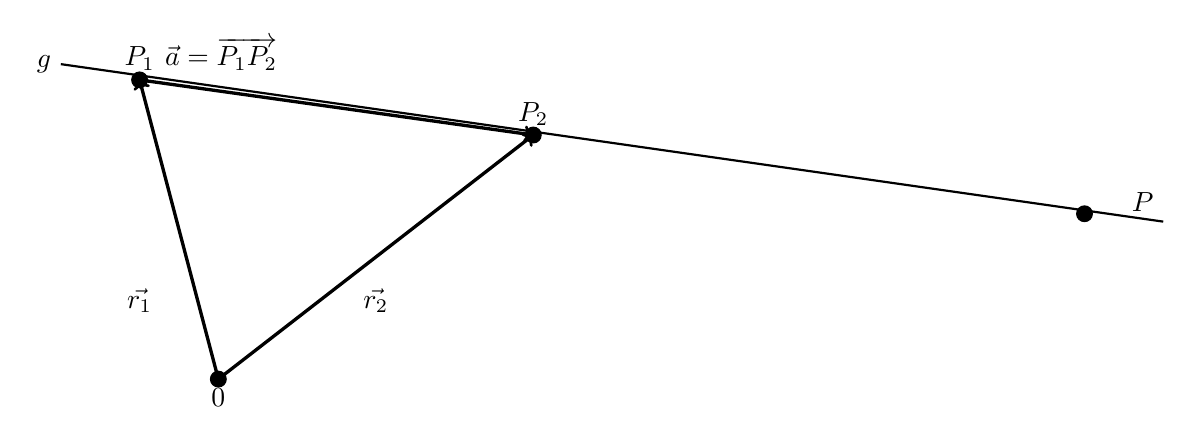
\begin{tikzpicture}[scale=2]
\node [below] at (0,0) {$0$}; \draw[fill] (0,0) circle [radius=0.05];
\draw [thick] (-1,2) -- (6,1); \node [left] at (-1,2) {$g$};

\draw[fill] (-0.5,1.9) circle [radius=0.05]; 
\node [above] at (-0.5,1.9) {$P_1$}; 
\draw [->,very thick] (0,0) -- (-0.5,1.9);
\node at (-0.5,0.5) {$\vec{r_1}$};

\draw[fill] (2,1.55) circle [radius=0.05]; 
\node [above] at (2,1.55) {$P_2$}; 
\draw [->,very thick] (0,0) -- (2,1.55);
\node at (1,0.5) {$\vec{r_2}$};

\node [above left] at (6,1) {$P$};
\draw[fill] (5.5,1.05) circle [radius=0.05]; 


\draw [->,very thick] (-0.5,1.9) -- (2,1.55); \node [above right] at (-0.4,1.9) {$\vec{a} = \overrightarrow{P_1P_2}$};
\end{tikzpicture}\\
$P \dots$ beliebiger Punkt von $g$\\
$\curvearrowright \overrightarrow{OP} = \overrightarrow{OP_1} + t \cdot \overrightarrow{P_1P_2}, t \in \mathbb{R}$\\
$\vec{r} = \vec{r_1} + t \cdot (\vec{r_2} - \vec{r_1}), t \in \mathbb{R}$\\
bzw.: $\vec{r} = \vec{r_1} = \vec{r_1} + t \cdot \vec{a}, t \in \mathbb{R}$
\item Parameterdarstellung einer Ebene $E$ durch drei Punkte $P_1, P_2, P_3$ die nicht auf einer Geraden liegen\\
$P \dots$ beliebiger Punkt von $E$.\\
$\overrightarrow{OP} = \overrightarrow{OP_1} + u \cdot \overrightarrow{P_1P_2} + v \cdot \overrightarrow{P_1P_3}, u,v \in \mathbb{R}$\\
$\vec{r} = \vec{r_1} + u \cdot (\vec{r_2} - \vec{r_1}) + v \cdot (\vec{r_3} - \vec{r_1} ) u,v \in \mathbb{R}$\\
$\vec{r} = \vec{r_1} + u \cdot \vec{a} + v \cdot \vec{b}, u,v, \in \mathbb{R}$
\item Parameterfreie Ebenengleichung\\
Normalvektor $\vec{n} (\vec{n} \neq \vec{0}, \vec{n} \perp E)$\\
$\vec{n} = \begin{pmatrix} a \\ b \\ c \end{pmatrix}, \vec{n} \perp \overrightarrow{P_0P}$\\
dabei $P(x,y,z) \dots$ beliebiger Punkt von $E$\\
$P_0 (x_0,y_0,z_0)$ fester Punkt von $E$\\
Orthogonal Kriterium $\curvearrowright (\vec{n}, \vec{r} - \vec{r_0} 0$ ausführlich:\\
$( \begin{pmatrix} a\\b\\c \end{pmatrix}, \begin{pmatrix} x-x_0\\ y - y_0 \\ z - z_0 \end{pmatrix}) = 0$ d.h. $a(x-x_0) + b\cdot (y-y_0) + c \cdot (z-z_0) = 0$\\
$\curvearrowright$ Allgemeine Form $ax+by+cz+d=0 \text{ mit } d= -ax_0 -by_0 -cz_0$
\end{enumerate}

\paragraph{Einige geometrische Grundaufgaben}
\begin{enumerate}
\item Schnitt Gerade und Ebene

Beispiel 16
\begin{equation}\label{EGG1}\text{Geg. Ebene }E: 2x -4y + z +3 = 0\end{equation}
\begin{equation}\label{EGG2}\text{Gerade } g: \begin{pmatrix}x\\y\\z\end{pmatrix} = \begin{pmatrix}3\\0\\1\end{pmatrix} + t \cdot \underbrace{\begin{pmatrix} -1 \\1 \\-2 \end{pmatrix}}_{\vec{a}}, t \in \mathbb{R} \end{equation}
Gesucht \begin{itemize}
\item Schnittpunkt $S(x_s,y_s,z_s)$
\item Schnittpunkt $\alpha$
\item $g: x=3-t y=t z=1-2t$
\end{itemize}
Einsetzen in (\ref{EGG1}) $\curvearrowright 2 \cdot (3-t) -4\cdot t + 1-2\cdot t +3 = 0$\\
$\curvearrowright -8t +10 = 0 \curvearrowright t = \frac{5}{4}$\\
Einsetzen in (\ref{EGG2}) $x=3 - \frac{5}{4} = \frac{7}{4}, y=\frac{5}{4} z= 1 - \frac{5}{2} = - \frac{3}{2}$\\
$\curvearrowright \underline{\underline{S(\frac{7}{4} | \frac{5}{4} | -\frac{3}{2} ) }}$\\
Seitenansicht\\
\begin{tikzpicture}
\node at (0,0) {E}; \draw (1,0) -- (7,0);
\node [above left]  at (3,0) {S};

\draw [->,very thick] (3,0) -- (3,4); \node [left] at (3,4) {$\vec{n}$};

\draw (1,-2) -- (6,3); \node [right] at (7,3) {g};
\node at (3.5,0.2) {$\alpha$};
\node at (3.3,0.6) {$\beta$};
\end{tikzpicture}\\
$\beta = \angle (\vec{n},\vec{a})$\\
$\alpha = \lvert 90^{\circ} - \beta \rvert$\\
\item Schnitt zweier Ebenen
\item Abstand $d(P_1,E)$ eines Punktes $P_1$ von einer Ebene $E$
\item Abstand $d(Q,g)$ eines Punktes $Q$ von einer Geraden $g$ \
$g: \vec{r} = \overrightarrow{0P_1} + t \vec{a}, t \in \mathbb{R}$\\
$L \dots $ Lotfuspunkt $ L \in g, \quad \overline{LQ} \perp g$\\
$d=$ Höhe $\overline{LQ}$ des von $\vec{a}$ und $\overrightarrow{P_1Q}$ auf gespannten Parallelogramms\\
$\curvearrowright d=d(Q,g) = \frac{\lvert \overrightarrow{P_1Q} \times \vec{a} \rvert}{\lvert \vec{a} \rvert }$ Lotfußpunkt $\overrightarrow{0L} = \overrightarrow{0P_1} + \underbrace{\overrightarrow{P_1Q}_{\vec{a}}}_{\text{Proj. von } \overrightarrow{P_1Q} \text{ auf } \vec{a}}$
\item Abstand $d(g_1,g_2)$ zweier nichtparalleler Geraden:\\
$g_1 : \vec{r} = \vec{r_1} + s \cdot \vec{a_1} (s\in \mathbb{R}$\\
$g_2 : \vec{r} = \vec{r_2} + t \cdot \vec{a_2} (t \in \mathbb{R} )$\\
$d=d(g_1,g_2) = \frac{\lvert ( \vec{r_2} - \vec{r_1} , \vec{a_1} \times \vec{a_2} ) \rvert }{\lvert \vec{a_1} \times \vec{a_2} \rvert }$
\end{enumerate}

\subsubsection{Transformationen im $\mathbb{R}^2$, homogene Koordinaten}
\begin{itemize}
\item Transformation eines Punktes $P(x,y) \mapsto P' (x',y')$ (neue Koordinaten im gleichen Koordinatensystem (= aktive Transformationen, wird im folgenden betrachtet)
\item eng verwandt: Transformation des Koordinatensystems $P(x,y)$ bleibt fest $\mapsto P'(x',y')$ neue Koordinaten in neuem Koordinatensystem (=passive Transformation)
\end{itemize}

\subparagraph{Translation} Verschiebung um den Vektor $\vec{t} = \begin{pmatrix}a \\b\end{pmatrix}$\\
\begin{equation}\label{Translation}
\begin{pmatrix} x' \\ y' \end{pmatrix} = \begin{pmatrix} x \\y \end{pmatrix} + \begin{pmatrix} a \\ b \end{pmatrix} 
\end{equation}

\subparagraph{Rotation} Zunächst Rotation um $0$, Drehwinkel $\alpha$\\
Es gilt: $x=r\cos{\varphi}, \; y=r \sin{\varphi}$\\*
($r,\varphi \dots$ Polarkoordinaten)\\
$x' = r \cos{(\varphi + \alpha)} = \underbrace{ r \cos{\varphi}}_{x} \cos{\alpha} - \underbrace{r \sin{\varphi}}_{y} \sin{\alpha}$\\
$\curvearrowright x' = x \cos{\alpha} - y \sin{\alpha}$\\*
analog $y' = x \sin{\alpha} + y \cos{\alpha}$\\
\[\begin{pmatrix} x' \\y'\end{pmatrix} = \underbrace{\begin{pmatrix} \cos{\alpha} - \sin{\alpha} \\ \sin{\alpha} \cos{\alpha} \end{pmatrix}}_{\text{Rotationsmatrix } \underline{R_{\alpha}}} \begin{pmatrix} x \\ y \end{pmatrix}\]

\subparagraph{Spiegelung} an einer Geraden $g$ durch $0$ mit dem Normaleneinheitsvektor $\vec{n} \; (\lvert \vec{n} \rvert = 1 )$\\
$\begin{pmatrix} x' \\ y' \end{pmatrix} = (\vec{E} - 2 \vec{n} \vec{n}^T ) \begin{pmatrix} x \\y \end{pmatrix}$ sogenannte \textsc{HouseHolder}-Matrix $\underline{H}$ (vgl. ÜA A6.23)

Bemerkung: Geradengleichung $ax + by + c = 0$
\[\curvearrowright \vec{n} = \frac{1}{\sqrt{a^2 + b2}} \begin{pmatrix} a \\ b \end{pmatrix}\]

\subparagraph{Skalierung (Zoom)} Koordinatenweise Streckung (oder Stauchung) von $0$ aus mit den Skalierungsfaktoren $u$ in $x$-Richtung, $v$ in $y$-Richtung
\[ \begin{pmatrix} x' \\ y' \end{pmatrix} = \underbrace{\begin{pmatrix} u & 0 \\ 0 & v \end{pmatrix}}_{\text{Skalierungsmatrix } \underline{S}_{u,v}} \begin{pmatrix} x \\ y \end{pmatrix} \]
speziell Spiegelung an x-Achse: $u=1, v=-1$\\*
speziell Spiegelung an y-Achse: $u=-1, v=1$\\

\subparagraph{Diskussion}
\begin{enumerate}
\item Drehungen um Punkte $\neq 0$ und Spiegelungen an Geraden nicht durch $0$ können durch Hintereinanderausführung einer Translation, Drehung bzw. Spiegelung und Rück-Translation realisiert.
\item Mit Ausnahme der Translation können die beschriebenen Transformationen durch Matrizen-Multiplikationen beschrieben werden (! lineare Abbildung) Zum Zwecke der Vereinheitlichung werden homogene Koordinaten eingeführt
\end{enumerate}

\subparagraph{Homogene 2D-Koordinaten} eines Punktes $P(x,y) : \begin{pmatrix} x \\ y \\1\end{pmatrix}$\\
(noch allgemeiner für $h \neq 0: \begin{pmatrix} hx\\hy\\h\end{pmatrix}$, kartesische Koordinaten ergeben sich dann durch Division durch die 3. Koordinate. Damit sind auch Zentralprojektionen beschreibar, im folgenden $h=1$)

\begin{itemize}
\item Translation in homogenen 2D-Koordinaten\\
Translationsvektor $\vec{t} = \begin{pmatrix} a \\b \end{pmatrix}$
\begin{equation}\label{HomoTrans}
\begin{pmatrix} x' \\ y' \\ 1\end{pmatrix} = \underbrace{\begin{pmatrix} 1 & 0 & a\\ 0 & 1 & b\\ 0 & 0 & 1 \end{pmatrix}}_{\text{Transformationsmatrix für homogene Koord } \underline{\tilde{T}}_{\underline{t}}} \begin{pmatrix} x \\ y \\ 1\end{pmatrix}
\end{equation}
Inverse ( $\triangleq$ Rück-Translation): $\underline{\tilde{T}}_t^{-1} = \underline{\tilde{T}}_{(-\vec{t})} = \begin{pmatrix} 1 & 0 & a\\ 0 & 1 & b\\ 0 & 0 & 1 \end{pmatrix}$
\item Rotation um $0$, Spiegelung an Geraden durch $0$, Skalierung in homogenen Koordinaten\\
Es sei $\underline{M}$ die Transformationsmatrix vom Typ $(2,2)$ für die kartesischen Koordinaten $\begin{pmatrix} x \\y \end{pmatrix}$. Dann ist die Transformationsmatrix für die homogenen Koordinaten:
\[ \underline{\tilde{M}} := \left( \begin{array}{c|c} \underline{M} & 0 \\ \hline 00 & 1\\ \end{array} \right) , \underline{\tilde{M}^{-1}} := \left( \begin{array}{c|c} \underline{M}^{-1} & 0 \\ \hline 00 & 1\end{array} \right) \]
\item Damit lässt sich die Hintereinanderausführung von beliebigen Translationen, Rotationen, Spiegelungen und Skalierungen durch Matrizenmultiplikationen darstellen (!nicht kommutativ). Die Gesamttransformation ist durch eine $(3,3)$-Matrix $\underline{\tilde{M}}$ darstellbar.
\item Mit einer weiteren Matrizenmultiplikation kann das Ergebnis der Gesamttransformation für $k$ Punkte $A(a_1,a_2),B(b_1,b_2),C(c_1,c_2), \dots $ erhalten werden:\\
$\underline{\tilde{M}} \cdot \bordermatrix{~ & A & B & C \cr
& a_1 & b_1 & c_1 & \dots \cr
&a_2 & b_2 & c_2 & \dots \cr
& 1 & 1 & 1 & \dots \cr} 
 =  \bordermatrix{~ & A' & B' & C' \cr
& a'_1 & b'_1 & c'_1 & \dots \cr
&a'_2 & b'_2 & c'_2 & \dots \cr
& 1 & 1 & 1 & \dots \cr}$ 
\end{itemize}

Beispiel 20: Das Dreieck $ABC$ mit $A(3,0), B(4,1) \text{ und } C(2,1)$ ist um seinen Eckpunkt $C$ um $60^\circ$ zu drehen (mathematisch positiv). Man gebe die Transformationsmatrix $\underline{\tilde{M}}$ für homogene 2D Koordinaten sowie das Bild an.\\
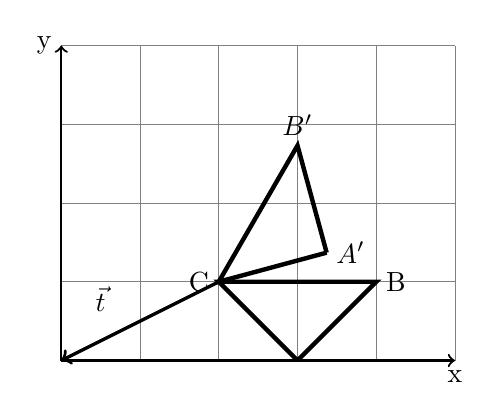
\begin{tikzpicture}
\draw[help lines] (0,0) grid (5,4); \draw [->,thick] (0,0) -- (0,4); \draw [->,thick] (0,0) -- (5,0); \node [left] at (0,4) {y}; \node [below] at (5,0) {x};

\draw [ultra thick] (3.37,1.37) -- (3,2.73) -- (2,1) -- (3.37,1.37);
\node [above] at (3,2.73) {$B'$}; \node [right] at (3.37,1.37) {$A'$};

\draw [ultra thick] (3,0) -- (2,1) -- (4,1) -- (3,0);
\node [right] at (4,1) {B}; \node [left] at (2,1) {C};

\draw [very thick, ->] (2,1) -- (0,0); \node [above] at (0.5,0.5) {$\vec{t}$};
\end{tikzpicture}
\begin{enumerate}
\item Translation um $\vec{t} = \begin{pmatrix} -2 \\-1\end{pmatrix}$\\
$\curvearrowright \underline{\tilde{T}}_{\vec{t}} = \begin{pmatrix}
1 & 0 & -2 \\
0 & 1 & -1 \\
0 & 0 & 1
\end{pmatrix}$
\item Rotation um $\alpha = 60^\circ$ um $0$\\
$\underline{R}_\alpha =  \begin{pmatrix} \cos{\alpha} & -\sin{\alpha}\\
\sin{\alpha} & \cos{\alpha} \end{pmatrix} = \begin{pmatrix}
\frac{1}{2} & -\frac{1}{2} \sqrt{3} \\
\frac{1}{2} \sqrt{3} & \frac{1}{2} \end{pmatrix}$\\
$\curvearrowright \underline{\tilde{R}}_\alpha = \begin{pmatrix}
\frac{1}{2} & -\frac{1}{2} \sqrt{3} & 0 \\
\frac{1}{2} \sqrt{3} & \frac{1}{2} & 0 \\
0 & 0 & 1 \end{pmatrix}$
\item Rücktranslation $\underline{\tilde{T}}_{\vec{-t}} = \begin{pmatrix}
1 & 0 & 2 \\
0 & 1 & 1 \\
0 & 0 & 1
\end{pmatrix}$
\end{enumerate}
$\curvearrowright \underline{\tilde{M}} = \underline{\tilde{T}}_{(-\vec{t})} \underline{R}_{\alpha} \underline{\tilde{T}}_{\vec{t}} $\\
$\curvearrowright A'(3,37;1,37), B'(3;2,73), C'(2;1)$

Bemerkung: Analoges Vorgehen im $\mathbb{R}^3$, homogene Koordinaten $x,y,z,1.$ Spiegelung an einer Ebene mit Normalen-Einheitsvektor $\vec{n}$ mit $(3,3)$- \textsc{HouseHolder}-Matrix.

Rotation um eine beliebige Achse (durch $0$) durch $3$ Drehungen um die Koordinatenachsen ersetzbar, \dots .\\
Anschließend erfolgt Projektion in $\mathbb{R}^2$

\subsubsection{Eigenwerte und Eigenvektoren}
Es sei $\underline{A}$ eine $(n,n)$-Matrix.

\subparagraph{Definition 13} Die Zahl $\lambda \in \mathbb{C}$ heißt Eigenwert (EW) der quadratischen Matrix $\underline{A}$, falls die Gleichung $\underline{A} \, \underline{x} = \lambda \underline{x}$ nicht triviale Lösungen $\underline{x} \quad (x \neq 0 )$ besitzt. Diese heißen dann Eigenvektoren (EV) von $\underline{A}$ zum EW $\lambda$.

Diskussion:
\begin{enumerate}
\item $\underline{A} \, \underline{x} = \lambda \underline{x} \Leftrightarrow (\underline{A} - \lambda \underline{E} ) \underline{x} = \underline{0}$ (homogenes System), d.h. nicht triviale Lösungen existieren genau dann, wenn $\det{(\underline{A} - \lambda \underline{E} )} = 0$ (charakteristische Gleichung) gilt.\\
\item $\curvearrowright$ Vorgehensweise zur Ermittlung von EW zu EV von $\underline{A}$
\begin{itemize}
\item charakteristische Gleichung lösen ($n \text{ im allg. komplexe Lösungen } \lambda_1 , \dots , \lambda_n ) \curvearrowright \text{ EW}$
\item Gleichungssysteme $\underline{A} - \lambda_i \underline{E} ) \underline{x} = \underline{0}$ lösen $\curvearrowright$ EV
\end{itemize}
\end{enumerate}

Im folgenden werden nur symmetrische $(n,n)$-Matrizen $\underline{S}$ betrachtet, d.h. $\underline{S}^T = \underline{S}$

\subparagraph{Satz 6} Es sei $\underline{S}$ symmetrische $(n,n)$-Matrix. Dann gilt:
\begin{enumerate}
\item Alle EW von $\underline{S}$ sind reell.
\item Zu verschiedenen EW $\lambda_1 \text{ bzw. } \lambda_2 (\lambda_1 \neq \lambda_2 )$ gehörende EV $\vec{v}_1 \text{ bzw. } \vec{v}_2$ sind orthogonal (vgl. Diskussion)
\item Es gibt eine Basis des Raumes $\mathbb{R}^n$, die aus $n$ paarweise orthonormierten EV $\vec{v}_1, \dots , \vec{v}_n$ von $\underline{S}$ besteht (vgl. Diskussion)
\item Es sei $\underline{V} = (\vec{v}_1; \vec{v}_2; \dots ; \vec{v}_n ) $ eine Matrix, die aus $n$ paarweise orthonormierten EV von $\underline{S}$ zusammengesetzt ist. Dann gilt:
\begin{itemize}
\item $\underline{V} \, \underline{V}^T = \underline{V}^T \underline{V} = \underline{E}$ (d.h. $\underline{V}^{-1} = \underline{V}^T$, $\underline{V}$ nennt sich auch orthogonale Matrix.
\item $\underline{V}^T \underline{S} \, \underline{V} = \begin{pmatrix}
\lambda_1 & 0 & \dots & 0\\
0 & \lambda_2 & \dots & 0\\
\vdots & \vdots & \ddots & \vdots \\
0 & 0 & \dots & \lambda_n \\
\end{pmatrix} = \Lambda$ (Diagonalmatrix)\\
$\curvearrowright \underline{S} = \underline{V} \, \underline{\Lambda} \underline{V}^T$
\item Es gilt $\underline{S}^{-1} = \underline{V} \, \underline{\Lambda}^{-1} \underline{V}^T$ (dabei $\underline{\Lambda}^{-1} = \begin{pmatrix}
\frac{1}{\lambda_1} & 0 & \dots & 0\\
0 & \frac{1}{\lambda_2} & \dots & 0\\
\vdots & \vdots & \ddots & \vdots \\
0 & 0 & \dots & \frac{1}{\lambda_n} \\
\end{pmatrix} \text{ und } \underline{S}^m = \underline{V} \underline{\Lambda}^m \underline{V}^T$
\end{itemize}

\end{enumerate}

Diskussion
\begin{enumerate}
\item Übertragung der Begriffe orthogonal, Länge eines Vektors aus $\mathbb{R}^3 \text{ bzw. } \mathbb{R}^2 \text{ in } \mathbb{R}^n$
\item $\vec{a}, \vec{b} \in \mathbb{R}^n$ heißen orthogonal, wenn $\vec{a}^T \vec{b} = \sum\limits_{i=1}^n a_i b_i = 0$ gilt, Skalarprodukt
\[ (\vec{a},\vec{b}) = \sum\limits_{i=1}^n a_i b_i\]
\item Betrag (Norm) eines Vektors $\lvert \vec{a} \rvert = \sqrt{\sum\limits_{i=1}^n a_i^2}$
\item paarweise orhtonomiert bedeutet 
\[ (\vec{v}_i,\vec{v}_j) = \left\{ \begin{array}{rcl}
         1
         & \mbox{falls}
         & i=j  \text{ d.h. } \lvert v_i \rvert = 1 (\forall i)\\ 
        0
         & \mbox{falls} 
         & i \neq j \\
                \end{array}\right.\]
\end{enumerate}

\subparagraph{Definition 13} \begin{enumerate}
\item $\underline{A} \, \vec{x} = \lambda \vec{x}, \, \vec{x} \neq \vec{0},\, \lambda \text{ EW }, \vec{x} \text{ EV}$
\item Veranschaulichung im Fall $n=2$:\\
Die symmetrische Matrix $\underline{A}$ habe die EW $\lambda_1$ und $\lambda_2$ und orthonormierte EV $\vec{v}_1$ und $\vec{v}_2, \underline{V} = (\vec{v}_1|\vec{v}_2)$\\
Es gilt: \\
$\underline{A} \vec{v}_1 = \lambda_1 \vec{v}_1$\\*
$\underline{A} \vec{v}_2 = \lambda_2 \underline{v}_2$\\
D.h. $\underline{A}$ bewirkt eine Skalierung mit den Faktoren $\lambda_1$ und $\lambda_2$ in Richtung $\vec{v}_1$ bzw. $\vec{v}_2$.

\end{enumerate}

\subparagraph{Definition 14} Es sei $\underline{S}$ eine reelle symmetrische Matrix vom Typ $(n,n)$. Die Funktion
\[ y= Q(\vec{x}) := \underbrace{\vec{x}^T}_{(1,n)} \underbrace{\underline{S}}_{(n,n)} \underbrace{\vec{x}}_{(n,1)} \quad (\vec{x} \in \mathbb{R}^n, y \in \mathbb{R})\]
heißt quadratische Form.

Diskussion:
\begin{enumerate}
\item Im Falle $n=2$ stellt $Q(\vec{x} ) = \text{ const. }$ (bzw. $ Q(\vec{x}) + \vec{a}^T \vec{x} = \text{ const. } )$ eine Kurve 2. Ordnung dar. Deren Gestalt kann durch die sogenannte Hauptachsentransformation ermittelt werden (vgl. Diskussion 3)
\item Ausführliche Schreibweise $\vec{x} = \begin{pmatrix} x \\y \end{pmatrix}, \underline{S} = \begin{pmatrix} s_{11} & s_{12}\\ s_{21} & s_{22} \end{pmatrix} \text{ mit } s_{12} = s_{21}$
\begin{equation}\label{Def14D2}
Q(x,y) = (x|y) \begin{pmatrix} s_{11} & s_{12} \\ s_{12} & s_{22} \end{pmatrix} \begin{pmatrix} x \\ y \end{pmatrix} = s_{11}x^2 + 2 s_{12} xy + s_{22} y^2
\end{equation}
\item Es seien $\lambda_1$ und $\lambda_2$ die EW von $\underline{S}$ und $\vec{v}_1$ bzw. $\vec{v}_2$ orthonomierte EV. Für einen beliebigen Vektor $\vec{x} = \begin{pmatrix} x \\y \end{pmatrix} \in \mathbb{R}^2$ seien $x^*,y^*$ die Koordinaten bzgl. der Basis 
\begin{equation} \label{Def14D31} \vec{v}_1,\vec{v}_2 : \vec{x} = x^* \cdot \vec{v}_1 + y^* \cdot \vec{v}_2 = (\vec{v}_1|\vec{v}_2 ) \begin{pmatrix} x^* \\ y^* \end{pmatrix} = \underline{V} \vec{x}^*
\end{equation} mit $\vec{x}^* = \begin{pmatrix} x* \\ y* \end{pmatrix}$. Dann gilt
\begin{equation}\label{Def14D32}
Q(x,y) = \lambda_1 x^{*2} + \lambda_2 y^{*2}
\end{equation} (Darstellung bzgl. der sog. Hauptachsen)

Denn: $Q(x,y) = \vec{x}^T \underline{S} \underline{x} = (\underline{V} \underline{x}^*)^T \underline{S} \underline{V} \vec{x}^* = \vec{x}^{*T} \underbrace{\underline{V}^T  \underline{S} \underline{V} \vec{x}^*}_{\Lambda \text{ vgl. Satz 6}} = (\vec{x}^* | \vec{y}^* ) \begin{pmatrix} \lambda_1 & 0 \\ 0 & \lambda_2 \end{pmatrix} \begin{pmatrix} x^* \\ y^* \end{pmatrix} = \lambda_1 x^{*2} + \lambda_2 y^{*2}$
\end{enumerate}

Beispiel 21: $Q(x,y) = 13x^2 - 32xy + 37y^2 = 45$\\
Welche Kurve?
\begin{itemize}
\item Matrix $\underline{S}$ (vgl. (\ref{Def14D2}), $\underline{S}= \begin{pmatrix} 13 & -16 \\ -16 & 37 \end{pmatrix} \quad ( s_{12} = -16 )$
\item charakteristische Gleichung: $\det{(\underline{S} - \lambda \underline{E})} \begin{vmatrix} 13-\lambda & -16 \\ -16 & 37 - \lambda \end{vmatrix} = 0 \Leftrightarrow \lambda^2 - 50 \lambda + 225 = 0 \curvearrowright \underline{\underline{\lambda_1 = 5, \lambda_2 = 45}} (\text{EW})$
\item EV zu $\lambda_1=5: 8x - 16y = 0 \curvearrowright x = 2y, y=t, x=2t (-16x + 32y = 0) \curvearrowright \underline{\underline{\begin{pmatrix} x \\y \end{pmatrix} = \begin{pmatrix} 2t \\ t \end{pmatrix} = t \cdot \begin{pmatrix} 2 \\ 1 \end{pmatrix}, t \neq 0 }}$
\item EV zu $\lambda_2 = 45: (-32x -16y = 0 ), -16x -8y = 0 \curvearrowright y=-2x, x=u, y= -2u \curvearrowright \underline{\underline{ \begin{pmatrix} x \\y \end{pmatrix} = \begin{pmatrix} u \\ -2u \end{pmatrix} = u \cdot \begin{pmatrix} 1 \\ -2 \end{pmatrix}, u \neq 0}}$
\item orthonormierte EV z.B: $\vec{v}_1 = \frac{1}{\sqrt{5}} \begin{pmatrix} 2 \\ 1 \end{pmatrix}, \vec{v}_2 = \frac{1}{\sqrt{5}} \begin{pmatrix}-1\\2\end{pmatrix}$ (Rechtssystem)
\end{itemize}
(\ref{Def14D32}) $\curvearrowright Q(x,y)= \lambda_1 x^{*2} + \lambda_2^{*2} = 5 x^{*2} + 45 y^{*2} = 45 \Leftrightarrow \frac{x^{*2}}{3^2} + \frac{y^{*2}}{1^2} =1$ Ellipse mit Halbachsen $a=3,b=1$

\section{Folgen, Reihen, Grenzwerte}
\subsection{Zahlenfolge}
\subsubsection{Grenzwerte von Zahlenfolgen}
\subparagraph{Definition 1}: Es sei $n_0 \in \mathbb{N}$. Eine Funktion $f$ mit $Db(f) = \{ n \in \mathbb{N} | n \geq n_0 \} \text{ und } Wb(f) \subseteq \mathbb{R}$ heißt reelle Zahlenfolge.\\
Schreibweisen: \[a_n := f(n)\]
$(a_n)_{n\geq n_0} = (a_{n_0}, a_{n_0 +1 }, a_{n_0 +2 },\dots)$\\
Oft ist $n_0 = 0$ oder $ n_0=1$.

\subparagraph{Beispiel 1}
\begin{enumerate}
\item $a_n = (-1)^n \cdot n (n \in \mathbb{N}), (a_n) = (0,-1,2,-3,4,-5,\dots)$
\item $a_0 = -1, a_n = n \cdot a_{n-1} ( n \in \mathbb{N}^*)$ (rekursive Definition)\\
$(a_n)= (-1,-1,-2,-6,-24,-120,\dots), a_n= -n!$
\item $a_n= \sum\limits_n \frac{3}{10^n} (n\in\mathbb{N}^*), (a_n) = (0,3;0,33;0,333;\dots)$
\item $a_n = a + (-1)^n \cdot \frac{1}{n^2} (n \in \mathbb{N}^*), (a_n) = (0,\frac{5}{4},\frac{8}{9},\frac{17}{16},\frac{24}{25},\dots)$
\end{enumerate}

\subparagraph{Definition 2}
\begin{itemize}
\item $(a_n)$ heißt konvergent, wenn es eine Zahl $a \in \mathbb{R}$ gibt mit:
\[\forall \epsilon >0 \; \exists n_0(\epsilon)\; (n_0 \in \mathbb{N}), \forall n \in \mathbb{N}_{\geq n_0(\epsilon)}: \lvert a_n - a \rvert < \epsilon\]
\item Die Zahl $a$ heißt Grenzwert von $(a_n)$.\\
Schreibweise $a= \lim\limits_{n \to \infty} a_n$
\item $(a_n)$ heißt divergent, wenn $(a_n)$ nicht konvergent ist.

Diskussion 
\item Folgen aus Beispiel 1\\
$\begin{array}{l|c|r}
\text{Folge} & \text{Monotonie} & \text{Beschränktheit}\\ \hline
a) \; a_n = (-1)^n n & - & - \\
b) \; a_n = -n! & \text{streng monoton fallend (ab } n=1) & -\\
c)\; a_n = \frac{3}{10} + \dots + \frac{3}{10^n} & \text{streng monoton wachsend} & 0,3 \leq a_n < \frac{1}{3} \\
d)\; a_n = 1 + (-1)^n \cdot \frac{1}{n^2} & - & 0 \leq a_n \leq \frac{5}{4}\\

\end{array}$
\end{itemize}

\subparagraph{Satz 1} Jede konvergente Folge ist beschränkt.
\subparagraph{Satz 2} Jede monotone und beschränkte Folge ist konvergent.

\subparagraph{Definition 5} $(a_n)$ heißt bestimmt divergent gegen $\left\{ \begin{array}{rc}
         +
         & \infty \\ 
        -
         & \infty\\
                \end{array}\right.$
falls gilt: $\forall C \in \mathbb{R} \exists n_0 (C) \forall n \geq n_0 (C) \left\{ \begin{array}{lc} a_n & > C \\ a_n & <C\\ \end{array} \right. $
\subparagraph{Satz 3} Jede unbeschränkte, monoton $\left\{ \begin{array}{l} \mbox{wachsende} \\ \mbox{fallende} \end{array} \right.$ Folge ist bestimmt divergent gegen $\left\{ \begin{array}{rc}
         + & \infty \\ 
        - & \infty\\
\end{array}\right.$\\
Schreibweise $\lim\limits_{n \to \infty} a_n = \left\{ \begin{array}{rc}
         + & \infty \\ 
        - & \infty\\
\end{array}\right.$

\subparagraph{Beispiel 2} \begin{enumerate}
\item Bsp 1 c) $a_n = \frac{3}{10} + \dots + \frac{3}{10^n}, (a_n)$ ist monoton wachsend und beschränkt $\underbrace{\Rightarrow}_{\text{Satz 2}} (a_n)$ ist konvergent, $\lim\limits_{n \to \infty} a_n = \frac{1}{3}$
\item Bsp 1 b) $a_n = -n!, (a_n)$ ist monoton fallend und unbeschränkt $\underbrace{\Rightarrow}_{\text{Satz 3}} (a_n)$ ist bestimmt divergent, $\lim\limits_{n \to \infty} a_n = - \infty$
\end{enumerate}

\subparagraph{Diskussion} Eine divergente Folge, die nicht bestimmt divergent ist, heißt unbestimmt divergent, z.B. Folge aus Beispiel 1a) $a_n = (-1)^n \cdot n$

\subparagraph{Einige wichtige Grenzwerte}
\begin{enumerate}
\item $\lim\limits_{n \to \infty} ( 1 + \frac{1}{n})^n = e$
\item $\lim\limits_{n \to \infty} \sqrt[n]{n} = 1$
\item $\lim\limits_{n \to \infty} \frac{\ln{n}}{n} = 0$
\item $\lim\limits_{n \to \infty} \sqrt[n]{a} = 1 \; (a > 0)$
\end{enumerate}

\subparagraph{Rechenregeln}(Grenzwertsätze)

\subparagraph{Satz4} $(a_n) \text{ und } (b_n)$ seien konvergente Folgen mit
$\lim\limits_{n \to \infty} a_n = a \text{ und } \lim\limits_{n \to \infty} b_n = b$.\\
Dann gilt
\begin{itemize}
\item $\lim\limits_{n \to \infty} ( a_n + b_n) = a+b,\quad \lim\limits_{n \to \infty} ( c \cdot a_n) = c \cdot a$
\item $\lim\limits_{n \to \infty} (a_n \cdot b_n) = a \cdot b, \quad \lim\limits_{n \to \infty} \frac{a_n}{b_n} = \frac{a}{b} \; (b \neq 0 )$
\end{itemize}

\subparagraph{Beispiel 3}
\begin{enumerate}
\item $a_n = \frac{2n^2 -1}{3n^2+n} ( n= 1,2,3,...)$\\
$a_n = \frac{n^2(2-\frac{1}{n^2})}{n^2 (3 + \frac{1}{n})} = \frac{2- \frac{1}{n^2}}{3+ \frac{1}{n}} \curvearrowright \lim\limits_{n\to \infty} a_n = \frac{2}{3}$\\
Ausklammern der jeweils höchsten Potenzen in Zähler und Nenner.
\item $a_n = n \cdot ( \sqrt{n^2 +1} -n)$\\
In Klammern "`$\infty - \infty$"' erweitern, 3. binomische Formel\\*
$= frac{n \cdot ( \sqrt{n^2 +1} -n) \cdot (\sqrt{n^2 +1} +n)}{\sqrt{n^2+1} +n}$\\
%$= \frac{n ( n^2 +1 -n^2)}{n \sqrt{n + \frac{1 + \frac{1}{n^2} + n}}}  = \frac{n}{n (\sqrt{1+\frac{1}{n^2}} +1)} = \frac{1}{\sqrt{1+\frac{1}{n^2}} +1} \underbrace{\implies}_{n \to \infty} \frac{1}{2}$ %Todo Fehler

\end{enumerate}

\subsubsection{Lineare Rekursionsgleichungen (Differenzgleichungen)}
\begin{itemize}
\item Allgemeine Form einer Rekursionsgleichung k-ter Ordnung $x_n = f (n, x_{n-1}, x_{n-2}, \dots,x_{n-k}),k \geq 1, n \geq n_0 + k$
\item Wir betrachten nur lineare Rekursionsgleichungen mit konstanten Koeffizienten (d.h. $a_j$ nicht von $n$ abhängig).

\begin{equation}\label{LRG1}
\begin{array}{c} x_n= a_1 x_{n-1} + a_2 x_{n-2} + \dots + a_k x_{n-k} + h_n \\
k \geq 1, a_k \neq 0, n \geq n_0 + k \end{array}
\end{equation}

\item Indexverschiebung möglich (z.B. um k)
\[ x_{n+k} = a_1 x_{n+k-1} + \dots + a_k x_n + h_{n+k}, \; n \geq n_0\]
Wichtig ist die Differenz zwischen höchsten und niedrigsten Index von $x$ (= Ordnung der Rekursionsgleichung)
\item  Die Differenzgleichung (\ref{LRG1}) heißt homogen, falls $h_n= 0(\forall n)$, sonst inhomogen
\end{itemize}

Zur Lösung von (\ref{LRG1})
\begin{enumerate}
\item Allgemeine Lösung von (\ref{LRG1}): \[x_n = x_n^{(h)} + x_n^{(p)}\] dabei ist $x_n^{(h)}$ die allgemeine Lösung der zugehörigen homogenen Gleichung
\begin{equation}\label{LRG2} x_n = a_1 x_{n-1} + \dots + a_k x_{n-k} \end{equation} und $x_n^{(P)}$ eine (partikuläre) Lösung der inhomogenen Gleichung (\ref{LRG1})
\item Es gibt $k$ Lösungen $x_n^{(1)}, \dots x_n^{(k)}$ der homogenen Gleichung, so dass gilt
\[x_n^{(h)} = c_1 x_n^{(1)} + \dots + c_k x_n^{(k)} \] gilt.\\
Diese erhält man mit Hilfe der Lösungen der charakteristischen Gleichung \begin{equation}\label{LRG3} \lambda^k = a_1 \lambda^{k-1} + a_2 \lambda^{k-2} + \dots + a_{k-1} \lambda + a_k \end{equation}
Diese ergibt sich aus dem Ansatz $x_n^{(h)} = \lambda^n \; ( \lambda \neq 0) \overbrace{\curvearrowright}^{(\ref{LRG2})} \lambda^n = a_1 \lambda^{n-1} + \dots + a_k \lambda^{n-k} | : \lambda^{n-k} \curvearrowright (\ref{LRG3})$\\
Bei $k$ verschiedenen Lösungen $\lambda_1, \dots, \lambda_k$ von (\ref{LRG3}) ergibt sich $x_n^{(h)} = c_1 \lambda_1^n + c_2 \lambda_2^n + \dots + c_k \lambda_k^n, \text{ falls z.B. } \lambda_2$ 2-fach auftritt, dann $x_n^{(h)}  = c_1 \lambda_1^n + c_2 \lambda_1^n \cdot n + \dots$
\item Für die Partikularlösung $x_n^{(P)}$ führen spezielle Ansätze zum Ziel:\\
\begin{tabular}{l|p{3cm}|p{4cm}}
Inhomogenität $h_n$ & Bedingung & Ansatz für $x_n^{(P)}$ \\ \hline
Polynom in $n$ (Grad $r$) & $\lambda = 1$ ist keine*) Lösung von (\ref{LRG3}) & Polynom vom gleichen Grade mit unbestimmten Koeffizienten \\
Potenzfunktion $b^n$ & $\lambda = b$ ist keine*) Lösung von (\ref{LRG3}) & $x_n^{(P)} = A \cdot b^n$\\
\end{tabular}
*) bei $\xi$-facher Lösung ist der Ansatz mit $n^\xi$ zu multiplizieren
\item unbestimmte Koeffizienten $A,\dots$ durch Einsetzen in die inhomogene Gleichung (\ref{LRG1}) und Koeffizientenvergleich ermitteln.
\item Die $k$ Konstanzen $C_1,\dots,C_k$ in der allgemeinen Lösung können durch die Anfangsbedingungen (A,B) (Vorgabe der ersten $k$ Glieder von $(x_n)$) ermittelt werden.
\end{enumerate}

Es sind also folgende Schritte durchzuführen
\begin{enumerate}
\item Allgemeine Lösung$x_n^{(h)}$ der homogenen Gleichung (\ref{LRG2}) ermitteln
\item eine spezielle Lösung $x_n^{(p)}$ der inhomogenen Gleichung (\ref{LRG1}) ermittlen
\item $x_n = x_n^{(h)} + x_n^{(p)}$
\item AB erfüllen
\end{enumerate}

Beispiel 4 $x_{n+1} = 2x_n + 3 \; n \geq 0, x_0 = 1$\\
Erste Glieder: $1,5,13,29,61, \dots$\\
Typ: Lineare Differenzengleichung 1. Ordnung\\

Lösung:
\begin{enumerate}
\item homogene Gleichung $x_{n+1} = 2x_n \text{ char. Gleichung } \lambda^1 = 2 \curvearrowright \lambda_1 = 2$
\item $h_n = 3$ (Polynom 0-ten Grades) $\curvearrowright$ Ansatz $x_n^{(p)}=A$\\
Einsetzen in Ausgangsleichung $A=2 \cdot A + 3 \curvearrowright A = -3$\\*
$\curvearrowright \underline{\underline{x_n^{(p)} = -3}}$
\item $x_n = x_n^{(h)} + x_n^{(p)} = \underline{\underline{C \cdot 2^n -3}}$
\item $AB: n=0 \curvearrowright x_0 =1 = C\cdot \underbrace{2^0}_{1} -3 \curvearrowright \underline{\underline{C=4}}$\\
Also: $\underline{\underline{x_n= 4 \cdot 2^n -3}}$
\end{enumerate}

Beispiel 5: $x_{n+2} = x_{n+1} + 2 x_n \; n \geq 0, x_0 =2 , x_1 = 3$\\
Erste Glieder: $2,3,7,13,27,53,\dots$\\
Typ: lineare homogene DifferenzGleichung 2. Ordnung
\begin{itemize}
\item Schritt $A$ liefert bereits die allg. Lösung ($B$ und $C$ entfallen)\\*
$\lambda^2 = \lambda +2 \curvearrowright \lambda_1 = -1, \lambda_2= 2 \curvearrowright x_n = x_n^{(h)} = c_1 \cdot (-1)^n + c_2 \cdot 2^n$

\item Schritt D: AB erfüllen\\
$n=0, \curvearrowright x_0 = 2 = C_1 + C_2$\\
$n=1 \curvearrowright x_1 = 3 = -C_1 + 2 C_2$\\
$\underline{\underline{C_2 = \frac{5}{3} , C_1 = \frac{1}{3}}}$\\
$\curvearrowright \text{ Lösung } \underline{\underline{x_n = \frac{1}{3} (-1)^n + \frac{5}{3} \cdot 2^n}}$
\end{itemize}

Diskussion: Bei einer homogenen linearen Differenzgleichung 2. Ordnung können folgende Fälle auftreten:
\begin{itemize}
\item $\lambda_1 , \lambda_2$ reell und verschieden\\
$\curvearrowright x_n = x_n^{(h)} = C_1 \lambda_1^n + C_2 \lambda_2^n$ (vgl. Beispiel 5)\\
\item $\lambda_1 = \lambda_2$ (reelle Doppellösung)\\
$\curvearrowright x_n = x_n^{(h)} = C_1 \lambda_1^n + C_2 n \lambda_1^n = \lambda_1^n (C_1 + C_2 \cdot n)$
\item $\lambda_{1,2} = u \pm iv (v \neq 0 )$ konjugiert komplexe Lösungen\\
\begin{equation}\label{DLD1} 
\curvearrowright x_n = x_n^{(h)} = C_1 \lambda_1^n + C_2 \lambda_2^n
\end{equation}
(wie im 1. Fall, die Koeffizienten $C_1 \text{ und } C_2$ sind aber im allg. komplex, $x_n$ selbst ist aber reell.
\end{itemize}

Reeller Ansatz ist mit Hilfe der Formeln von \textsc{Euler} und \textsc{Moivre} möglich:\\
$\lambda_1^n = (r e^{i \varphi})^n = r^n e^{in\varphi} = r^n(\cos{(n\varphi)} + i \sin{(n \varphi)})$\\
$\lambda_2^n = (r e^{-i \varphi})^n = r^n e^{-in\varphi} = r^n(\cos{(n\varphi)} - i sin{(n \varphi)})$\\
Damit reeller Ansatz:
\begin{equation}\label{DLD2}
x_n = x_n^{(h)} = K_1 r^n \cos{(n \varphi)} + K_2 r^n \sin{(n \varphi)}
\end{equation}
Bemerkung: Falls Rechner mit komplexer Arithmetik vorhanden, so ist (\ref{DLD1}) bequemer.

\subsubsection{Unendliche Reihen}
\paragraph{Grundbegriffe}
\subparagraph{Definition 6}
\begin{itemize}
\item Geg. Zahlenfolge $(a_n) n \geq n_0, n_0 \in \mathbb{N}$\\
Die Zahlenfolge $(s_n)_{n\geq n_0}$ mit\\
$s_{n_0} := a_{n_0}, s_{n_0 +1} := a_{n_0} + a_{n_0 + 1}, s_{n_0 +2}, s_n := a_{n_0} + a_{n_0+1} + \dots + a_n , \dots$ (Partialsummenfolge)\\
heißt unendliche Reihe. Bezeichnung: $\sum\limits_{n=n_0}^{\infty} a_n$
\item Ist die Reihe konvergent, d.h. Folge $(s_n)$ ist konvergent, so heißt $s:= \lim\limits_{n\to \infty} s_n =: \sum\limits_{n=n_0}^{\infty} a_n$ die Summe der Reihe.
\item Die Reihe heißt (bestimmt oder unbestimmt) divergent, wenn die Partialsummenfolge die entsprechende Eigenschaft hat.
\end{itemize}

Beispiel 6: $a_n = a \cdot q^n \quad a \neq 0, q \neq 0, n=0,1,2,\dots$\\
d.h. $(a_n) = (a,aq,aq^2,aq^3,\dots)$\dots gemetrische Folge\\
Quotient zweier aufeinanderfolgender Glieder\\
$\frac{a_{n+1}}{a_n} = q$ \dots Quotient\\
$(s_n) = \sum\limits_{n=0}^{\infty} a q^n$ \dots unendliche geometrische Reihe
\begin{itemize}
\item $s_0 = a, s_1 = a + aq, s_2 a + aq +aq^2, \dots$\\
$\begin{array}{r|c}
(1) & s_n = a + aq + \dots + aq^n |\cdot q\\
(2) & s_n \cdot q = aq + \dots + aq^n + aq^{n+1}\\ \hline
(1)-(2) & s_n(1-q) = a(1-q^{n+1})\\
\end{array}$\\
$\curvearrowright s_n = a \cdot \frac{1-q^{n+1}}{1-q}$ (falls $q \neq 1$)
(Summenformel für die endliche geometrische Reihe, dabei $a$ \dots Anfangsglied, $q$ \dots Quotient, Anzahl der Summanden $n+1$)
\item $\curvearrowright \lim\limits_{n \to \infty} s_n = \frac{a}{1-q} \quad (\text{ für } \lvert q \rvert < 1)$
$\curvearrowright$ Summe der unendlichen geometrischen Reihe
\[ s = \sum\limits_{n=0}^{\infty} a \cdot q^n = \frac{a}{1-q} \quad \text{ für } \lvert q \rvert < 1\]
Anwendung z.B. periodischer Bruch: $0,\overline{72} = 0,7272727272... = \frac{72}{100} + \frac{72}{100^2} + \frac{72}{100^3} + ... = \frac{\frac{72}{100}}{1-\frac{1}{100}} = \underline{\underline{\frac{72}{99}}} = \underline{\underline{\frac{8}{11}}}$\\
allg. $q=b^{-p}$ dabei $b$ \dots Basis $p$\dots Periodenlänge, hier ($q=10^{-2} = \frac{1}{100})$
\end{itemize}

Beispiel 7: $\sum\limits_{n=1}^{\infty} \frac{1}{n} = a + \frac{1}{2} + \frac{1}{3} + \dots$ harmonische Reihe\\
Offensichtlich ist $(s_n)$ (streng) monoton wachsend. Man kann zeigen, dass $s_n$ nicht beschränkt ist.\\
Damit folgt aus Satz 3: Die harmonische Reihe ist bestimmt divergent.
(Schreibweise: $\sum\limits_{n=1}^{\infty} \frac{1}{n} = \infty$)

\subparagraph{Definition 7} Die Reihe $\sum\limits_{n=n_0}^{\infty} a_n$ heißt 
\begin{enumerate}
\item absolut konvergent, falls $\sum\limits_{n=n_0}^{\infty} \lvert a_n\rvert$ konvergent
\item bedingt konvergent falls $\sum\limits_{n=n_0}^{\infty} a_n$ konvergent $\wedge \sum\limits_{n=n_0}^{\infty} \lvert a_n \rvert$ divergent
\end{enumerate}

\subparagraph{Satz 5} $\sum\limits_{n=n_0}^{\infty} a_n$ absolut konvergent $\Rightarrow \sum\limits_{n=n_0}^{\infty} a_n$ konvergent

Diskussion
\begin{enumerate}
\item Die Umkehrung gilt im allgemeinen nicht. Es gibt konvergente Reihen, die nicht absolut konvergent sind.\\
z.B. $\sum\limits_{n=1}^{\infty} (-1)^{n-1} \cdot \frac{1}{n}$
\item Für Reihen mit nicht negativen Gliedern $a_n \geq 0$ ist absolute Konvergent identisch mit (gewöhnlicher) Konvergenz (klar weegen $\lvert a_n \rvert = a_n$). Für solche Reihen gilt entweder $\sum\limits_{n=n_0}^{\infty} a_n < \infty$, d.h. (absolute) Konvergenz oder (XOR) $\sum\limits_{n=n_0}^{\infty} a_n = \infty$,d.h. bestimmte Divergenz
\end{enumerate}
























\end{document}